% !TeX program = pdflatex
% ENG 101 Programming for Engineers: From Formulas to Programs
% Compile with:  latexmk -pdf main.tex
\documentclass[12pt,a4paper,oneside,openany]{book}
% Book metadata.
\newcommand{\BookTitle}{From Formulas to Programs}
\newcommand{\BookCoverTitle}{From Formulas\\to Programs}
\newcommand{\BookSubtitle}{How Engineers Compute in Python, Fortran, C, MATLAB and More}
\newcommand{\BookShortTitle}{From Formulas to Programs}
\newcommand{\ProjectVersion}{(ENG 101, Fall 2026, version 1.0.1)}
\newcommand{\ProjectDate}{18 November 2026}
\newcommand{\ProjectStatus}{Reading notes}
\newcommand{\BookAuthor}{Yanwei Wang}
\newcommand{\BookAffiliation}{School of Engineering, Nazarbayev University}

% Portable pdfLaTeX setup. Uses standard TeX Live fonts; no font files supplied.
\usepackage[T1]{fontenc}
\usepackage[utf8]{inputenc}
\usepackage[english]{babel}
\usepackage[fontsize=12.2pt]{scrextend}
\usepackage{lmodern}
\usepackage[sc]{mathpazo}
\usepackage{helvet}
\renewcommand{\ttdefault}{lmtt}
\usepackage[a4paper,left=22mm,right=22mm,top=22mm,bottom=22mm,headheight=16pt,headsep=7mm,footskip=12mm]{geometry}
\usepackage{microtype,amsmath,amssymb,xspace}
% Typewriter text must stay plain ASCII: no << >> -- ligatures in code set outside listings.
\DisableLigatures[<,>,-,`,',\,]{encoding = T1, family = tt*}
\usepackage{textcomp}
\usepackage{setspace}
\setstretch{1.055}
\usepackage{xcolor}
% Colour edition (for reading on screen). The grayscale print palette is in the
% Best Practices reader; only the definitions in this block differ.
\definecolor{ink}{HTML}{1B2430}      % text and main headings
\definecolor{accent}{HTML}{12497A}   % deep blue
\definecolor{gold}{HTML}{C8922A}
\definecolor{muted}{HTML}{5A6675}
\definecolor{pale}{HTML}{EEF3F8}     % light blue tint
\definecolor{warm}{HTML}{FBF4E6}
\definecolor{mint}{HTML}{FFFFFF}
\definecolor{okgreen}{HTML}{2E7D5B}
\definecolor{palegreen}{HTML}{EDF6F1}
\definecolor{alert}{HTML}{B5483A}
\definecolor{palealert}{HTML}{FBEFEC}
\definecolor{paleslate}{HTML}{F1F3F5}
\definecolor{codebg}{HTML}{F7F8FA}
\definecolor{codeframe}{HTML}{D5DAE0}
\definecolor{codegreen}{HTML}{4F7A5A}
\definecolor{coderust}{HTML}{A8452E}
\definecolor{navy}{HTML}{0E2A47}
\usepackage{graphicx,float,rotating}
\usepackage{xurl,ragged2e}
\definecolor{mint}{gray}{1}
\usepackage{tikz,pgfplots}
\usetikzlibrary{arrows.meta,positioning,calc,shapes.geometric,fit,backgrounds}
\pgfplotsset{compat=1.18}
\usepackage{booktabs,longtable,tabularx,array}
\renewcommand{\tabularxcolumn}[1]{>{\RaggedRight\arraybackslash}p{#1}}
\usepackage[font=small,labelfont={sf,bf,color=ink},labelsep=period,skip=8pt]{caption}
\usepackage{enumitem}
\setlist{leftmargin=*,topsep=6pt,itemsep=5pt,parsep=2pt}
\usepackage{titlesec}
\newcommand{\BookChapterLabel}{CHAPTER}
\titleformat{\chapter}[display]
 {\sffamily\bfseries\color{ink}\raggedright\hyphenpenalty=10000\exhyphenpenalty=10000}
 {\color{gold!85!black}\fontsize{13}{17}\selectfont \BookChapterLabel\ \thechapter}
 {10pt}{\fontsize{25}{29}\selectfont}[\vspace{7pt}{\color{gold}\rule{30mm}{2.2pt}}]
\titlespacing*{\chapter}{0pt}{4pt}{22pt}
\titleformat{\section}{\sffamily\bfseries\Large\color{accent}}{\thesection}{0.65em}{}
\titlespacing*{\section}{0pt}{17pt plus 3pt}{7pt}
\titleformat{\subsection}{\sffamily\bfseries\large\color{ink}}{\thesubsection}{0.65em}{}
\titlespacing*{\subsection}{0pt}{12pt plus 2pt}{5pt}
\usepackage{fancyhdr}
\pagestyle{fancy}
\fancyhf{}
\fancyhead[L]{\footnotesize\sffamily\color{muted}\nouppercase{\leftmark}}
\fancyfoot[L]{\footnotesize\sffamily\color{muted}\BookShortTitle}
\fancyfoot[R]{\sffamily\bfseries\color{accent}\thepage}
\renewcommand{\headrulewidth}{0.6pt}\renewcommand{\headrule}{{\color{gold}\hrule width\headwidth height\headrulewidth}}
\renewcommand{\chaptermark}[1]{\markboth{\thechapter\quad #1}{}}
\fancypagestyle{plain}{\fancyhf{}\fancyfoot[L]{\footnotesize\sffamily\color{muted}\BookShortTitle}\fancyfoot[R]{\sffamily\bfseries\color{accent}\thepage}\renewcommand{\headrulewidth}{0pt}}
\usepackage[most]{tcolorbox}
\tcbset{enhanced,breakable,arc=0.8mm,boxrule=0.35pt,colframe=accent!35,left=10pt,right=10pt,top=8pt,bottom=8pt,before skip=10pt,after skip=11pt}
\newtcolorbox{researchquestion}{colback=pale,borderline west={1.5pt}{0pt}{accent},fontupper=\itshape}
\newtcolorbox{sourcepanel}{colback=black!3,fontupper=\small}
\newtcolorbox{practicebox}[1]{colback=mint,colframe=accent!35,title={\IfBeginWith{#1}{Practice}{#1}{Practice: #1}},colbacktitle=mint,coltitle=ink,fonttitle=\sffamily\bfseries,borderline west={1.5pt}{0pt}{accent},titlerule=0pt}
\newtcolorbox{readerroute}{colback=pale,borderline west={1.5pt}{0pt}{accent},fontupper=\small,title={Reading route},colbacktitle=pale,coltitle=ink,fonttitle=\sffamily\bfseries,titlerule=0pt}
\newtcolorbox{workedexample}[1]{colback=mint,colframe=accent!35,title={\IfBeginWith{#1}{Worked example}{#1}{Worked example: #1}},colbacktitle=mint,coltitle=ink,fonttitle=\sffamily\bfseries,borderline west={1.5pt}{0pt}{accent},titlerule=0pt}
\usepackage{listings}
\lstset{basicstyle=\small\ttfamily,breaklines=true,columns=fullflexible,keepspaces=true,showstringspaces=false,frame=single,rulecolor=\color{black!20},xleftmargin=5pt,xrightmargin=5pt,aboveskip=10pt,belowskip=10pt}
\usepackage{needspace}
\usepackage{etoolbox}
\pretocmd{\section}{\Needspace{8\baselineskip}}{}{\PackageError{booksetup}{Cannot protect section headings}{}}
\pretocmd{\subsection}{\Needspace{5\baselineskip}}{}{\PackageError{booksetup}{Cannot protect subsection headings}{}}
\usepackage{csquotes,xstring}
\usepackage[authoryear,round]{natbib}
\let\parencite\citep
\let\textcite\citet
\usepackage{makeidx}
\makeindex

\usepackage[colorlinks=true,linkcolor=accent,citecolor=accent,urlcolor=accent,unicode=true,bookmarksnumbered=true]{hyperref}
\usepackage{bookmark}
\hypersetup{pdftitle={\BookTitle: \BookSubtitle},pdfauthor={\BookAuthor},pdfsubject={ENG 101 Programming for Engineers, reading notes},pdfkeywords={programming languages, engineering, Python, course notes}}
\setcounter{tocdepth}{0}
\setcounter{secnumdepth}{1}
\setlength{\parindent}{0pt}
\setlength{\parskip}{5pt plus 1pt}
\setlength{\emergencystretch}{3em}
\renewcommand{\arraystretch}{1.20}
\setlength{\tabcolsep}{5pt}
\setlength{\textfloatsep}{15pt plus 3pt minus 2pt}
\setlength{\intextsep}{13pt plus 3pt minus 2pt}
\clubpenalty=10000
\widowpenalty=10000
\raggedbottom
% Larger secondary text than the default 12pt book class, especially figure labels.
\makeatletter
\renewcommand\small{\@setfontsize\small{10.8}{13.2}}
\renewcommand\footnotesize{\@setfontsize\footnotesize{10}{12.2}}
\renewcommand\scriptsize{\@setfontsize\scriptsize{9}{10.7}}
\makeatother
\newcommand{\Field}[2]{\par\noindent\textbf{#1}\ #2\par}
\newcommand{\OnePageHeading}[1]{\section*{#1}}
\newcommand{\ProjectChapter}[2]{\chapter*{#1}\markboth{#1}{}\phantomsection\addcontentsline{toc}{chapter}{#1}\label{#2}}
\newcommand{\PlanSection}[2]{\section{#1}#2\par}
\newcommand{\BookPart}[3]{%
 \clearpage\refstepcounter{part}\markboth{#1}{}%
 \addcontentsline{toc}{part}{\thepart\space #1}\thispagestyle{plain}%
 \vspace*{22mm}{\sffamily\bfseries\color{accent}\Large PART \thepart\par}%
 \vspace{9mm}{\sffamily\bfseries\color{ink}\fontsize{31}{37}\selectfont\raggedright\hyphenpenalty=10000\exhyphenpenalty=10000 #1\par}%
 \vspace{9mm}{\color{accent}\rule{\textwidth}{1pt}\par}%
 \vspace{6mm}{\large #2\par}\vspace{10mm}#3\par\vfill\clearpage}
\newcounter{casebrief}
\renewcommand{\thecasebrief}{\Alph{casebrief}}
\newcommand{\CaseChapter}[1]{\clearpage\refstepcounter{casebrief}\chapter*{Case \thecasebrief: #1}\markboth{Case \thecasebrief: #1}{}\addcontentsline{toc}{chapter}{Case \thecasebrief: #1}\label{case:\thecasebrief}}
\newcommand{\CaseRef}[1]{Case~\ref{case:#1}}
\newcommand{\CheckField}[2]{\textbf{#1} & #2\\\addlinespace[5pt]}
\newcommand{\WritingPrompt}[1]{\begin{sourcepanel}\textbf{Writing prompt.} #1\end{sourcepanel}}

% Full titles in Contents/bookmarks, compact titles only in running heads.
\newcommand{\BookChapter}[2][]{\chapter{#2}\if\relax\detokenize{#1}\relax\else\chaptermark{#1}\fi}
\newcommand{\ExerciseLevel}[1]{{\sffamily\small\color{accent}[#1]}\enspace}

% Extensions for a programming book. Load after booksetup.tex. Colour edition.
\colorlet{nublue}{accent}
\colorlet{nugold}{gold}
% ---------------- listings: languages not built in --------------------
\lstdefinelanguage{JavaScript}{
  morekeywords={break,case,catch,class,const,continue,debugger,default,delete,do,
    else,export,extends,finally,for,function,if,import,in,instanceof,let,new,
    return,super,switch,this,throw,try,typeof,var,void,while,with,yield,
    async,await,of,null,true,false,undefined,static,get,set},
  morecomment=[l]{//}, morecomment=[s]{/*}{*/},
  morestring=[b]', morestring=[b]", morestring=[b]`,
  sensitive=true}
\lstdefinelanguage{TypeScript}[]{JavaScript}{
  morekeywords={interface,type,enum,implements,private,public,protected,readonly,
    number,string,boolean,any,void,never,unknown}}
\lstdefinelanguage{Julia}{
  morekeywords={abstract,begin,break,catch,const,continue,do,else,elseif,end,export,
    false,finally,for,function,global,if,import,let,local,macro,module,mutable,
    quote,return,struct,true,try,using,while,in,where,nothing},
  morecomment=[l]{\#}, morecomment=[s]{\#=}{=\#},
  morestring=[b]", sensitive=true}
\lstdefinelanguage{Rust}{
  morekeywords={as,break,const,continue,crate,else,enum,extern,false,fn,for,if,impl,
    in,let,loop,match,mod,move,mut,pub,ref,return,self,Self,static,struct,super,
    trait,true,type,unsafe,use,where,while,f64,f32,i32,i64,u32,u64,usize,bool,
    String,Vec,Option,Some,None,Result,Ok,Err},
  morecomment=[l]{//}, morecomment=[s]{/*}{*/}, morestring=[b]", sensitive=true}
\lstdefinelanguage{Go}{
  morekeywords={break,case,chan,const,continue,default,defer,else,fallthrough,for,
    func,go,goto,if,import,interface,map,package,range,return,select,struct,
    switch,type,var,float64,int,string,bool,true,false,nil,error},
  morecomment=[l]{//}, morecomment=[s]{/*}{*/},
  morestring=[b]", morestring=[b]`, sensitive=true}
\lstdefinelanguage{StructuredText}{
  morekeywords={PROGRAM,END_PROGRAM,VAR,END_VAR,VAR_INPUT,VAR_OUTPUT,IF,THEN,ELSIF,
    ELSE,END_IF,FOR,TO,BY,DO,END_FOR,WHILE,END_WHILE,CASE,OF,END_CASE,
    FUNCTION_BLOCK,END_FUNCTION_BLOCK,FUNCTION,END_FUNCTION,BOOL,INT,REAL,TIME,
    TRUE,FALSE,AND,OR,NOT,TON,R_TRIG},
  morecomment=[s]{(*}{*)}, morecomment=[l]{//}, morestring=[b]', sensitive=false}
\lstdefinelanguage{Modelica}{
  morekeywords={model,end,parameter,Real,equation,der,initial,algorithm,annotation,
    connector,flow,extends,import,within,package,block,input,output,constant},
  morecomment=[l]{//}, morecomment=[s]{/*}{*/}, morestring=[b]", sensitive=true}
\lstdefinelanguage{VBA}{
  morekeywords={Sub,End,Function,Dim,As,Double,Integer,Long,String,For,To,Next,If,
    Then,Else,ElseIf,Do,While,Loop,Set,Range,Cells,Return,Exit,Step,Boolean,
    Const,Private,Public,Wend,Variant},
  morecomment=[l]{'}, morestring=[b]", sensitive=false}
\lstdefinelanguage{GCode}{
  morekeywords={G00,G01,G02,G03,G17,G21,G90,G91,M03,M05,M30,G0,G1,F,S},
  morecomment=[s]{(}{)}, morecomment=[l]{;}, sensitive=false}


% ---------------- listings: house style for a code-heavy book -----------
% 10 pt code (\footnotesize in this setup) keeps about 88 characters per line.
\lstset{basicstyle=\footnotesize\ttfamily,keywordstyle=\bfseries\color{accent},
  commentstyle=\itshape\color{codegreen},stringstyle=\color{coderust},
  backgroundcolor=\color{codebg},rulecolor=\color{codeframe},
  upquote=true,tabsize=4,postbreak={\mbox{$\hookrightarrow$\space}},
  extendedchars=true,
  literate={-}{-}1 {*}{*}1 {σ}{{$\sigma$}}1 {ε}{{$\varepsilon$}}1 {π}{{$\pi$}}1
    {μ}{{$\mu$}}1 {ρ}{{$\rho$}}1 {α}{{$\alpha$}}1 {Δ}{{$\Delta$}}1 {°}{{$^\circ$}}1}
\lstdefinestyle{numbered}{numbers=left,numberstyle=\scriptsize\sffamily\color{muted},numbersep=7pt,xleftmargin=20pt}
% program output: pale blue panel with a blue bar
\lstdefinestyle{output}{language={},frame=leftline,framerule=2pt,rulecolor=\color{accent},
  backgroundcolor=\color{pale},basicstyle=\footnotesize\ttfamily\color{ink},
  keywordstyle={},commentstyle={},stringstyle={},xleftmargin=8pt}
% terminal commands: dark panel with light text
\lstdefinestyle{shell}{language={},frame=single,rulecolor=\color{navy},backgroundcolor=\color{navy},
  basicstyle=\footnotesize\ttfamily\color{white},keywordstyle={},
  commentstyle={\itshape\color{white!60!navy}},stringstyle={}}
% \codefile[opts]{language}{path under code/}{note}  and  \outfile[opts]{path under code/}
\newcommand{\codefile}[4][]{\lstinputlisting[language={#2},style=numbered,
  title={\footnotesize\sffamily\bfseries\color{accent}\texttt{\detokenize{#3}}\normalfont\sffamily\color{muted}\enspace #4},#1]{code/#3}}
\newcommand{\outfile}[2][]{\lstinputlisting[style=output,title={\footnotesize\sffamily\color{muted}Output},#1]{code/#2}}

% ---------------- boxed notes: one shape, one colour per kind ---------------
% \begin{notebox}{title}{main colour}{background}
\newtcolorbox{notebox}[3]{colback=#3,colframe=#2!40,title={#1},colbacktitle=#3,coltitle=#2!85!black,
  fonttitle=\sffamily\bfseries,borderline west={2.5pt}{0pt}{#2},titlerule=0pt,boxrule=0.35pt}
\newenvironment{keyidea}[1][Key idea]{\begin{notebox}{#1}{accent}{pale}}{\end{notebox}}
\newenvironment{pitfall}[1][Common pitfall]{\begin{notebox}{#1}{alert}{palealert}}{\end{notebox}}
\newenvironment{engnote}[1][Engineering note]{\begin{notebox}{#1}{gold}{warm}}{\end{notebox}}
\newenvironment{history}[1][A little history]{\begin{notebox}{#1}{muted}{paleslate}}{\end{notebox}}
\newenvironment{tryit}[1][At the computer]{\begin{notebox}{Practice: #1}{okgreen}{palegreen}}{\end{notebox}}
\renewtcolorbox{researchquestion}{colback=pale,colframe=accent!40,borderline west={2.5pt}{0pt}{gold},
  fontupper=\itshape\color{accent!80!black}}
% Language fact sheet: blue title bar, pale panel, two columns.
\newenvironment{factsheet}[1]{\begin{tcolorbox}[colback=pale,colframe=accent,boxrule=0.5pt,
  title={#1 at a glance},colbacktitle=accent,coltitle=white,fonttitle=\sffamily\bfseries,titlerule=0pt,
  left=8pt,right=8pt]
  \small\renewcommand{\arraystretch}{1.12}%
  \begin{tabular}{@{}>{\leavevmode\sffamily\bfseries\color{accent}}p{.22\linewidth}>{\RaggedRight\arraybackslash}p{.73\linewidth}@{}}}
  {\end{tabular}\end{tcolorbox}}

% ---------------- exercises: "Try it yourself", linked to the answers ------
\newcounter{exercise}[chapter]
\renewcommand{\theexercise}{\thechapter.\arabic{exercise}}
\newcommand{\exitem}{\refstepcounter{exercise}\label{ex:\theexercise}%
  \textbf{\sffamily\color{accent}Exercise \theexercise.}}
\newenvironment{exercises}{\section*{Try it yourself}%
  \begin{list}{\exitem}{\leftmargin=0pt\itemindent=0pt\labelwidth=0pt\labelsep=0.5em\itemsep=7pt\topsep=4pt\listparindent=0pt
  \renewcommand{\makelabel}[1]{##1}}}{\end{list}}
\newcommand{\AnswerRef}[1]{\hyperref[ex:#1]{\textsf{Exercise #1}}}

% ---------------- shorthand ------------------------------------------------
\newcommand{\py}{Python\xspace}
\newcommand{\code}[1]{\texttt{#1}}
\newcommand{\sq}{\textquotesingle}   % straight quote for inline code
\newcommand{\file}[1]{\texttt{#1}}
\newcommand{\term}[2][]{\textbf{\color{accent}#2}\if\relax\detokenize{#1}\relax\index{#2}\else\index{#1}\fi}
\newcommand{\unit}[1]{\,\mathrm{#1}}
\newcommand{\LearningOutcomes}[1]{\par\textbf{\color{accent}Learning outcomes.} #1\par}

% Line under the question box of Chapters 4--14
\newcommand{\OrientationNote}{\par{\small\sffamily\color{muted}Orientation chapter: read it to recognise the language and what it is for, not to memorise its syntax.}\par}

\begin{document}
\frontmatter
\hypersetup{pageanchor=false}
% Cover page: full-page TikZ drawing. Needs two pdfLaTeX runs (latexmk does this).
\begin{titlepage}
\thispagestyle{empty}
\newcommand{\CoverAt}[2]{($(current page.north west)+(#1mm,-#2mm)$)}
\newcommand{\CoverLine}[3]{% y position, language, code
  \node[anchor=base west,font=\sffamily\bfseries\fontsize{10.5}{12}\selectfont,text=gold] at \CoverAt{34}{#1} {#2};
  \node[anchor=base west,font=\ttfamily\fontsize{11}{12}\selectfont,text=white] at \CoverAt{62}{#1} {\detokenize{#3}};}
\begin{tikzpicture}[remember picture,overlay]
% background
\fill[navy] (current page.south west) rectangle (current page.north east);
\fill[accent!55!navy] \CoverAt{0}{0} rectangle \CoverAt{210}{9};
\fill[gold] \CoverAt{0}{9} rectangle \CoverAt{210}{10.2};
% faint drag curve (the running example) across the page, with Euler points
\begin{scope}[shift={($(current page.north west)+(24mm,-258mm)$)},x=8.1mm,y=0.62mm]
  \draw[white,opacity=0.25,line width=0.5pt] (0,0) -- (20,0) (0,0) -- (0,62);
  \node[anchor=south east,font=\sffamily\fontsize{8.5}{10}\selectfont,text=gold,opacity=0.8,inner sep=1.5pt] at (20,56.03) {terminal velocity};
  \node[anchor=north east,font=\sffamily\fontsize{8.5}{10}\selectfont,text=white,opacity=0.45,inner sep=2pt] at (20,0) {time};
  \node[anchor=north west,rotate=90,font=\sffamily\fontsize{8.5}{10}\selectfont,text=white,opacity=0.45,inner sep=2pt] at (0,2) {speed};
  \draw[gold,opacity=0.45,dashed,line width=0.8pt] (0,56.03) -- (20,56.03);
  \draw[white,opacity=0.55,line width=1.6pt,domain=0:20,samples=80,smooth]
     plot (\x,{56.03*tanh(9.81*\x/56.03)});
  \foreach \t/\v in {0/0,1/9.73,2/19.10,3/27.59,4/34.59,5/40.26,6/44.74,7/48.02,8/50.44,
     9/52.16,10/53.36,11/54.19,12/54.77,13/55.16,14/55.44,15/55.63,16/55.76,17/55.84,
     18/55.90,19/55.94,20/55.97}
     \fill[gold,opacity=0.75] (\t,\v) circle[radius=1.5pt];
\end{scope}
% series label
\node[anchor=west,font=\sffamily\bfseries\fontsize{10.5}{12}\selectfont,text=gold] at \CoverAt{24}{27}
  {\textls[140]{ENG 101 \textperiodcentered\ PROGRAMMING FOR ENGINEERS}};
% title
\node[anchor=north west,align=left,text=white,font=\sffamily\bfseries\fontsize{54}{62}\selectfont,inner sep=0pt]
  at \CoverAt{24}{44} {\BookCoverTitle};
\fill[gold] \CoverAt{24}{99} rectangle \CoverAt{66}{100.6};
\node[anchor=north west,align=left,text=white!85!navy,font=\sffamily\fontsize{18}{25}\selectfont,inner sep=0pt,text width=160mm]
  at \CoverAt{24}{108} {How Engineers Compute in Python, Fortran, C,\\MATLAB and More};
% "editor window": the same line of the running example in six languages
\fill[black,opacity=0.28,rounded corners=3mm] \CoverAt{25.5}{149.5} rectangle \CoverAt{188.5}{214.5};
\fill[navy!62!black,rounded corners=3mm] \CoverAt{24}{148} rectangle \CoverAt{187}{213};
\fill[white,opacity=0.07,rounded corners=3mm] \CoverAt{24}{148} rectangle \CoverAt{187}{159};
\fill[alert!85!white] \CoverAt{31}{153.5} circle[radius=1.5mm];
\fill[gold] \CoverAt{36.5}{153.5} circle[radius=1.5mm];
\fill[okgreen!85!white] \CoverAt{42}{153.5} circle[radius=1.5mm];
\node[anchor=base,font=\sffamily\fontsize{9.5}{11}\selectfont,text=white!60!navy] at \CoverAt{105.5}{154.8}
  {one Euler step for a falling skydiver};
\CoverLine{168.5}{Python}{v[n+1] = v[n] + dt*(g - c/m*v[n]**2)}
\CoverLine{176.3}{Fortran}{v(n+1) = v(n) + dt*(g - c/m*v(n)**2)}
\CoverLine{184.1}{C, C++}{v[n+1] = v[n] + dt*(g - c/m*v[n]*v[n]);}
\CoverLine{191.9}{MATLAB}{v(n+1) = v(n) + dt*(g - c/m*v(n)^2);}
\CoverLine{199.7}{R}{v[n+1] <- v[n] + dt*(g - c/m*v[n]^2)}
\CoverLine{207.5}{Julia}{v[n+1] = v[n] + dt*(g - c/m*v[n]^2)}
% author block
\node[anchor=north west,align=left,inner sep=0pt,text=white,font=\sffamily\bfseries\fontsize{19}{23}\selectfont]
  at \CoverAt{24}{268} {\BookAuthor};
\node[anchor=north west,align=left,inner sep=0pt,text=white!78!navy,font=\sffamily\fontsize{11.5}{15}\selectfont]
  at \CoverAt{24}{277} {Department of Chemical and Materials Engineering\\\BookAffiliation};
\node[anchor=north east,align=right,inner sep=0pt,text=white!78!navy,font=\sffamily\fontsize{11.5}{15}\selectfont]
  at \CoverAt{186}{277} {{\bfseries\color{gold}\ProjectStatus}\\Fall 2026 \textperiodcentered\ \ProjectDate};
\end{tikzpicture}
\end{titlepage}

\hypersetup{pageanchor=true}
\ProjectChapter{How to Use These Notes}{guide:reader}
A structural engineer opens a finite-element package and finds that its solver was written
in Fortran and C++. A process engineer inherits a spreadsheet full of VBA macros. A test
bench in the laboratory runs MATLAB scripts, the controller on the production line is
programmed in a language called Structured Text, and the dashboard that displays the plant
data is written in JavaScript. All of them learned to program in one language, and all of
them now have to read several.

You are learning to program in \py. That is the right first language for an engineer in
2026: it is free, readable, and used everywhere from data analysis in a chemical plant to
the control software of a research robot. These notes are a map of the other languages you
will meet. They do not replace the \py lectures and laboratories; read them alongside.
Each chapter introduces one language or a family of related languages: where it came
from, what engineers use it for, how to write and run a first program, how its basic
building blocks look, and what it is good and bad at. Every language chapter solves the
same small engineering problem, so that you can compare the languages line by line.

The title, \emph{From Formulas to Programs}, names what all these languages are for. An
engineer starts with a formula or a physical law and needs a program that computes with
it. Fortran, the oldest language in these notes, took its name from exactly this step:
\emph{formula translation}. The \hyperref[epilogue]{Epilogue} follows that idea from 1957
to the present and beyond.

\section*{Why learn about several languages?}

You will write most of your code in one or two languages. So why read about ten?
There are three practical reasons.

\begin{enumerate}
\item \textbf{You will read more code than you write.} Engineers inherit code:
  a Fortran solver from the 1990s, a MATLAB toolbox from a former student,
  a C driver for a sensor. Being able to read such code, even slowly, and
  recognise what it does is a real professional skill.
\item \textbf{Concepts transfer; syntax does not matter much.} Variables, loops,
  functions, arrays and files exist in every language. Once you see the same idea
  written five ways, you understand the idea, not just the \py spelling of it.
  This makes your \py better, too.
\item \textbf{Choosing the right tool is an engineering decision.} A spreadsheet
  macro, a \py script and a C++ program can all compute a heat-exchanger
  design. Which one you should choose depends on who will use it, how fast it must
  run, how long it must live and what hardware it runs on. You can only make that
  choice if you know the options.
\end{enumerate}

\section*{Choose a starting point}
\textbf{If you read only part of these notes.} Read Chapters 1--3, Chapter 16 and the
Epilogue carefully. Use Chapters 4--15 as a map: read them to recognise each language and
what it is for, not to memorise its syntax.
\par\textbf{Start with the foundations (Chapters 1--2).} Chapter~\ref{ch:intro} explains what a
programming language is and how languages differ. Chapter~\ref{ch:howcoderuns} explains how
code is turned into something a computer can execute, and how numbers are stored. Both
prepare you for everything that follows.
\par\textbf{Study \py carefully (Chapter 3).} Chapter~\ref{ch:python} is the longest
chapter and follows the order of topics in the course. Use it to revise.
\par\textbf{Read the other language chapters for orientation (Chapters 4--14).} You do not
need to memorise their syntax. Read each one with a question in mind: \emph{how is this
language different from \py, and why?} The exercises can be done with free tools.
\par\textbf{Compare and choose (Chapters 15--16).} Chapter~\ref{ch:rosetta} solves the same
three tasks in thirteen languages side by side. Chapter~\ref{ch:choosing} discusses how to
choose a language and how to write code that others can trust. The Epilogue closes with
the history and the likely future of the languages of engineering.
\par\textbf{Type the examples.} Reading code is good; running and changing it is much
better. Every complete program in these notes is short enough to type in a few minutes,
and all of them are in the \file{code} folder of the repository named at the end of this
guide.

\section*{Read the page}
A complete program is printed with its file name and with line numbers:
\begin{lstlisting}[language=Python,style=numbered,title={\footnotesize\sffamily\bfseries\color{accent}\texttt{python/hello.py}\normalfont\sffamily\color{muted}\enspace a first script}]
print("Hello, engineers!")
\end{lstlisting}
What the program prints follows on a pale blue panel with a blue bar at the left. It is
the real output of the program, not a retyped copy:
\begin{lstlisting}[style=output,title={\footnotesize\sffamily\color{muted}Output}]
Hello, engineers!
\end{lstlisting}
Commands that you type into a terminal (the ``command line'') are shown on a dark panel.
The \texttt{\$} sign is the prompt; do not type it.
\begin{lstlisting}[style=shell]
$ python3 hello.py
\end{lstlisting}
These commands are written for Linux and macOS. On Windows, use the Windows Subsystem for
Linux (WSL) or one of the browser-based options; both are explained in the guide
\hyperref[app:install]{Installing and Running the Languages} at the back.
Short fragments inside the text have a frame but no file name. They illustrate one point
and may need surrounding code before they run.

Boxed notes come in five colours:
\begin{keyidea}
A concept to understand and remember.
\end{keyidea}
\begin{engnote}
How the topic matters in real engineering work.
\end{engnote}
\begin{pitfall}
A mistake that beginners, and experienced programmers, often make.
\end{pitfall}
\begin{history}
Where a language or an idea came from.
\end{history}
\begin{tryit}
A short activity to do at the computer.
\end{tryit}
Each chapter ends with exercises under the heading \emph{Try it yourself}. Hints and
answers to selected exercises are at the back; click an exercise number there to jump
back to the question.

\section*{Follow one example through every language}
\label{sec:runningexample}

To compare languages fairly we will solve the same problem in each of them. The problem
is one you know from Newtonian mechanics. A skydiver of mass $m$ falls from rest.
Gravity pulls down with force $mg$; air resistance pushes up with a force that grows
with the square of the speed, $c v^2$, where $c$ is a drag coefficient (in kg/m).
Newton's second law gives
\begin{equation}
  m\frac{dv}{dt} = mg - c v^2, \qquad v(0) = 0.
  \label{eq:drag}
\end{equation}
When the two forces balance, the acceleration is zero and the speed stops growing.
This \emph{terminal velocity} is
\begin{equation}
  v_\mathrm{t} = \sqrt{\frac{mg}{c}}.
  \label{eq:vterminal}
\end{equation}
Equation~\eqref{eq:drag} happens to have an exact solution,
\begin{equation}
  v(t) = v_\mathrm{t}\tanh\!\left(\frac{g t}{v_\mathrm{t}}\right),
  \label{eq:dragexact}
\end{equation}
which lets us check a numerical answer. The numerical method we use is the simplest one
there is, the \emph{explicit Euler method}. We replace the derivative by a finite
difference over a small time step $\Delta t$:
\begin{equation}
  \frac{v_{n+1} - v_n}{\Delta t} \approx g - \frac{c}{m} v_n^2
  \quad\Longrightarrow\quad
  v_{n+1} = v_n + \Delta t\left(g - \frac{c}{m}v_n^2\right).
  \label{eq:euler}
\end{equation}
Starting from $v_0 = 0$ we apply this update again and again. Each application moves
time forward by $\Delta t$. In every language chapter we use the same numbers:
$m = 80\unit{kg}$, $c = 0.25\unit{kg/m}$, $g = 9.81\unit{m/s^2}$, a time step
$\Delta t = 0.5\unit{s}$, and we stop at $t = 20\unit{s}$. With these numbers
$v_\mathrm{t} = \sqrt{80 \times 9.81/0.25} \approx 56.03\unit{m/s}$.

The program in each language does four things that almost every engineering program does:
\begin{enumerate}
\item it stores some \textbf{parameters} in variables;
\item it defines a \textbf{function} (the right-hand side $g - (c/m)v^2$);
\item it uses a \textbf{loop} to step forward in time and stores the results in an
  \textbf{array};
\item it \textbf{prints} a formatted table and compares with the exact answer.
\end{enumerate}
Figure~\ref{fig:dragresult} shows the result. You will see this curve many times.

\begin{figure}[htbp]
\centering
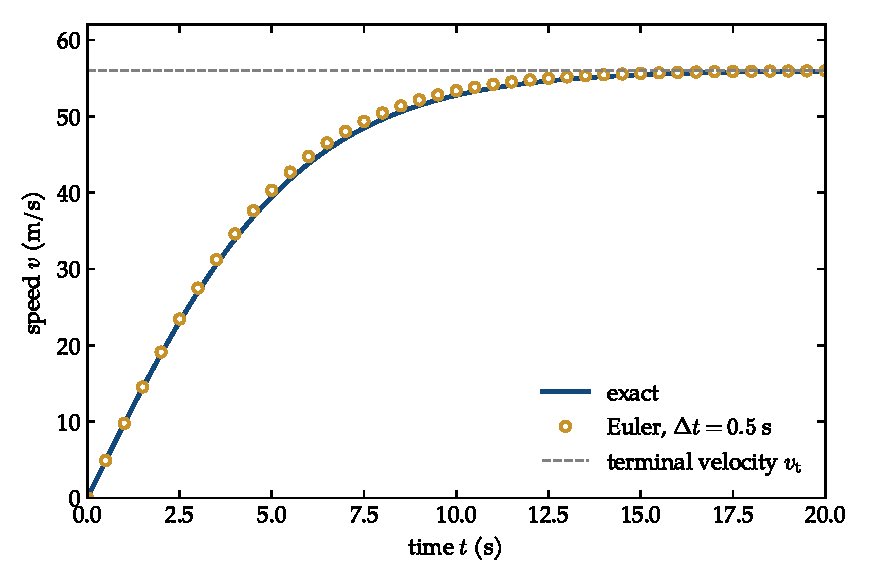
\includegraphics[width=0.72\linewidth]{figures/drag_euler.pdf}
\caption[{The running example}]{The running example. Speed of a falling skydiver with quadratic air drag ($m=80\unit{kg}$,
$c=0.25\unit{kg/m}$). The solid line is the exact solution~\eqref{eq:dragexact};
the markers are the Euler method with $\Delta t = 0.5\unit{s}$. The dashed line is the
terminal velocity. Every language chapter reproduces this calculation.}
\label{fig:dragresult}
\end{figure}

\section*{About these notes}
Reading notes for ENG 101 Programming for Engineers (6 ECTS), Nazarbayev University, Fall
2026. Version 1.0.1, 18 November 2026; corrections are
listed in the file \file{ERRATA.md} of the repository. \copyright\ 2026 Yanwei Wang. The notes are provided to students of ENG 101 for study.
MATLAB examples were tested in GNU Octave, which runs the same core language, and the
C\# examples with the Mono compiler. The Wolfram Language programs were run in
Mathematica and the Julia programs in Julia 1.13. Only the short fragments in
Chapter~\ref{ch:others} (VBA, Structured Text, Verilog, VHDL, Modelica, G-code), which need
special tools, were checked by hand and were not run. The data files used in the examples
contain invented teaching values, not measurements. All programs, data files and the
source of these notes are at \url{https://github.com/ktwyw/from-formulas-to-programs};
the script \file{tools/check\_examples.py} there re-runs every program and compares its
output with the output printed in these notes. Contact:
\texttt{yanwei.wang@nu.edu.kz}; ORCID 0000-0002-8488-9833.

\section*{Acknowledgements}
These notes grew out of questions asked by ENG 101 students: \emph{``Why do we learn
\py and not C?''}, \emph{``Is MATLAB still used?''}, \emph{``What language does my
calculator use?''}. Thank you for asking them. Comments, corrections and suggestions are
very welcome; please send them by email.

\par\medskip\hfill Yanwei Wang, Astana, November 2026

{\setlength{\parskip}{0pt}\tableofcontents}
\mainmatter
% =====================================================================
\phantomsection
\addcontentsline{toc}{part}{Foundations}
\BookChapter[What Is a Programming Language?]{What Is a Programming Language?}
\label{ch:intro}

\begin{researchquestion}
What is a programming language, and why do engineers need so many different ones?
\end{researchquestion}
% =====================================================================

A computer is a machine that follows instructions very fast and very exactly. It does
not guess what you meant. A \term{programming language} is an artificial language,
with strict rules of spelling and grammar, that lets a person write those instructions
down in a form that can be turned into something the machine can execute. The written
instructions are called a \term{program}, or \term{source code}.

This chapter introduces the vocabulary we need to talk about languages: algorithms,
levels of abstraction, programming paradigms, type systems, and the main language
families. It ends with a short history and a table of which languages are used in which
branch of engineering.

\LearningOutcomes{Describe an algorithm separately from the language it is written in; place a language on the scale from machine code to domain-specific tools; recognise the main programming paradigms in a short piece of code; explain the difference between static and dynamic typing and between compiling and interpreting; and read a popularity ranking with the right amount of caution.}

\section{Algorithms come first}

Before there is a program there is an \term{algorithm}: a finite list of precise steps
that solves a problem. The idea is much older than computers. The Euclidean algorithm for
the greatest common divisor of two integers is more than 2000 years old:

\begin{enumerate}
\item Take two positive integers $a$ and $b$.
\item If $b = 0$, the answer is $a$. Stop.
\item Otherwise replace $(a, b)$ by $(b, a \bmod b)$, where $a\bmod b$ is the remainder
  of $a/b$, and go back to step 2.
\end{enumerate}

For $a = 1071$, $b = 462$ the steps give $(1071, 462) \to (462, 147) \to (147, 21)
\to (21, 0)$, so the answer is $21$. The algorithm is the same in every language. Here
it is in \py,
\begin{lstlisting}[language=Python]
def gcd(a, b):
    while b != 0:
        a, b = b, a % b
    return a
\end{lstlisting}
and here it is in C:
\begin{lstlisting}[language=C]
int gcd(int a, int b) {
    while (b != 0) {
        int r = a % b;
        a = b;
        b = r;
    }
    return a;
}
\end{lstlisting}
The two programs look different: C wants to know that \code{a} and \code{b} are
integers (\code{int}), it uses braces \code{\{ \}} to mark blocks and semicolons to end
statements, and it needs a temporary variable \code{r} for the swap. \py marks blocks
by indentation and can swap two values in one line. But the \emph{algorithm} is
identical. Keep this in mind when you read the rest of these notes: most of what
differs between languages is \emph{notation}; the ideas are shared.

\begin{keyidea}
Think about the algorithm first, and the language second. If you can describe the steps
of a solution clearly in words or with a flowchart, writing them in any language is a
matter of looking up the notation.
\end{keyidea}

\section{From problem to program: pseudocode and flowcharts}

Experienced programmers rarely start by typing code. They first describe the algorithm in
a form that is independent of any language. Two tools are common.

\paragraph{Pseudocode} is a precise, structured description in plain language, using the
building blocks that every language has (variables, decisions, loops). Here is Newton's
method for solving $f(x) = 0$, which we will meet in every language chapter:
\begin{lstlisting}[language={},basicstyle=\ttfamily\small,keywordstyle={},
  morekeywords={INPUT,OUTPUT,SET,FOR,TO,IF,THEN,RETURN,END,STOP,REPORT}]
INPUT  function f, derivative df, starting guess x0, tolerance tol, max_iter
SET x = x0
FOR k = 1 TO max_iter
    SET step = f(x) / df(x)
    SET x = x - step
    IF |step| < tol THEN
        RETURN x and k
    END IF
END FOR
REPORT "no convergence" and STOP
\end{lstlisting}

\paragraph{Flowcharts} show the same logic as a diagram (Figure~\ref{fig:flowchart}).
Ovals mark the start and end, rectangles are actions, diamonds are decisions, and arrows
show the order. Flowcharts are particularly helpful for logic with many branches, such as
the control sequence of a machine, and they are the ancestors of the graphical languages
described in Chapter~\ref{ch:others}.

\begin{figure}[htbp]
\centering
\begin{tikzpicture}[node distance=6mm and 10mm,
  every node/.style={font=\sffamily\small},
  term/.style={draw=nublue,fill=nublue!8,rounded corners=8pt,minimum width=26mm,minimum height=7mm},
  act/.style={draw=nublue,fill=white,minimum width=34mm,minimum height=7mm,align=center},
  dec/.style={draw=nugold!85!black,fill=nugold!10,diamond,aspect=2.4,inner sep=1pt,align=center},
  arr/.style={-{Stealth[length=2.2mm]},thick}]
\node[term] (start) {start};
\node[act,below=of start] (init) {read $f$, $f'$, $x_0$\\set $x = x_0$, $k = 0$};
\node[act,below=of init] (step) {$k = k + 1$\\$s = f(x)/f'(x)$, \ $x = x - s$};
\node[dec,below=of step] (conv) {$|s| < \mathrm{tol}$?};
\node[term,right=18mm of conv] (done) {output $x$, $k$};
\node[dec,below=of conv] (maxit) {$k \ge k_\mathrm{max}$?};
\node[term,right=18mm of maxit] (fail) {report failure};
\draw[arr] (start) -- (init);
\draw[arr] (init) -- (step);
\draw[arr] (step) -- (conv);
\draw[arr] (conv) -- node[above]{yes} (done);
\draw[arr] (conv) -- node[right]{no} (maxit);
\draw[arr] (maxit) -- node[above]{yes} (fail);
\draw[arr] (maxit.west) -- node[above]{no} ++(-14mm,0) |- (step.west);
\end{tikzpicture}
\caption{Flowchart of Newton's method with a stopping tolerance and a maximum number of
iterations.}
\label{fig:flowchart}
\end{figure}

Whichever tool you use, a good algorithm description answers four questions before any code
is written: What are the inputs, and in which units? What are the outputs? What steps
transform one into the other? And how will I check that the answer is right? The last
question is the one beginners most often forget.

\section{From switches to Python: levels of abstraction}

A processor (CPU) understands only \term{machine code}: sequences of binary numbers,
each of which encodes a very simple operation such as ``add the numbers in two
registers'' or ``jump to address 4096 if the last result was zero''. Writing programs
directly in machine code is possible but extremely tedious and error-prone. Over the
decades, programmers built layers of languages on top of machine code, each layer
hiding more detail.

\begin{figure}[htbp]
\centering
\resizebox{\linewidth}{!}{%
\begin{tikzpicture}[
  layer/.style={draw=nublue,fill=nublue!#1,minimum width=10.5cm,minimum height=0.85cm,
    font=\sffamily\small,align=center,rounded corners=2pt},
  node distance=1.5mm]
\node[layer=5]  (l5) {\textbf{Domain-specific languages}: SQL, MATLAB/Simulink, Modelica, spreadsheet formulas};
\node[layer=10, below=of l5] (l4) {\textbf{High-level, interpreted / JIT}: \py, R, JavaScript, Julia, Wolfram};
\node[layer=18, below=of l4] (l3) {\textbf{High-level, compiled}: Fortran, C++, Java, C\#, Rust, Go};
\node[layer=28, below=of l3] (l2) {\textbf{``Portable assembly''}: C};
\node[layer=40, below=of l2] (l1) {\textbf{Assembly language}: \texttt{mov}, \texttt{add}, \texttt{jmp} \ldots};
\node[layer=55, below=of l1,text=white] (l0) {\textbf{Machine code}: \texttt{10110000 01100001} \ldots};
\draw[-{Stealth[length=3mm]},thick,nugold] ([xshift=6mm]l0.east) -- node[right,font=\sffamily\small,align=left]{more\\abstract,\\closer to\\the problem} ([xshift=6mm]l5.east);
\draw[-{Stealth[length=3mm]},thick,nugold] ([xshift=-6mm]l5.west) -- node[left,font=\sffamily\small,align=right]{more\\control,\\closer to\\the hardware} ([xshift=-6mm]l0.west);
\end{tikzpicture}}
\caption{Levels of programming languages. Higher levels let you express the problem
more directly; lower levels give you more control over what the hardware does.}
\label{fig:levels}
\end{figure}

\subsection*{The processor understands only machine code}

To see what ``low level'' means, consider adding two numbers. In \py you write
\code{c = a + b}. In x86-64 assembly language the same thing could look like this:
\begin{lstlisting}[language={[x86masm]Assembler}]
    mov  eax, DWORD PTR [rbp-4]    ; load a from memory into register eax
    add  eax, DWORD PTR [rbp-8]    ; add b to it
    mov  DWORD PTR [rbp-12], eax   ; store the result in c
\end{lstlisting}
Each line is one instruction for the processor. An \term{assembler} translates each
instruction into its binary machine code. Assembly is specific to one processor family:
code for an Intel laptop does not run on the ARM processor in your phone. Today
assembly is used only where every clock cycle or every byte counts, for example in the
start-up code of a microcontroller or in the innermost loops of a numerical library.

\subsection*{A high-level language hides the machine}

A \term{high-level language} lets you write \code{c = a + b} and leaves the details
(which registers to use, where in memory to put \code{c}) to a translator program. The
first widely used high-level language was \textbf{Fortran} (1957), designed at IBM for
scientists and engineers who wanted to write formulas, not machine instructions. Its name
is short for \emph{FORmula TRANslation}. Chapter~\ref{ch:fortran} tells its story.

High-level languages bring three big advantages:
\begin{itemize}
\item \textbf{Productivity}: one line of high-level code can replace dozens of machine
  instructions.
\item \textbf{Portability}: the same source code can be translated for different
  processors.
\item \textbf{Readability}: other people (and you, six months later) can understand the
  program.
\end{itemize}
The price is that you give up some control. The translator decides how to use the
hardware, and it may not make the choice you would have made. For most engineering work
this is a very good trade.

\section{Programming paradigms}

A \term{paradigm} is a style of organising a program. Most modern languages support
several paradigms, but each language has a ``natural'' style. Knowing the paradigms helps
you understand why languages look the way they do.

\subsection*{Imperative programs change state step by step}

In the \term{imperative} style a program is a sequence of commands that change the
\emph{state} of the computer (the values stored in variables). ``Set \code{x} to 0. Add 1
to \code{x}. If \code{x} is less than 10, repeat.'' \term[procedural programming]{Procedural} programming
organises those commands into named \emph{procedures} (also called functions or
subroutines) that can be called again and again. Fortran, C, and the scripts you write in
the first weeks of ENG 101 are procedural.
\begin{lstlisting}[language=Python]
# Procedural style: a function that changes nothing outside itself
def mean(values):
    total = 0.0
    for v in values:
        total = total + v
    return total / len(values)
\end{lstlisting}

\subsection*{Objects bundle data with the functions that use them}

In \term{object-oriented programming} (OOP) data and the functions that work on that data
are bundled together into \term{objects}. A \term{class} is a blueprint for objects. For
example, a class \code{Pipe} could store a length, a diameter and a roughness, and offer
a method \code{pressure\_drop(flow\_rate)}. Each actual pipe in a network is an object (an
\term{instance}) of that class. C++, Java and C\# are built around OOP; \py supports it
fully.
\begin{lstlisting}[language=Python]
class Pipe:
    def __init__(self, length, diameter):
        self.length = length        # m
        self.diameter = diameter    # m

    def area(self):
        return 3.141592653589793 * self.diameter**2 / 4

p = Pipe(length=12.0, diameter=0.05)
print(p.area())                     # 0.0019634954084936207
\end{lstlisting}
Three ideas usually come with OOP:
\begin{itemize}
\item \term{encapsulation}: the inside of an object is hidden; you use it through its
  methods;
\item \term{inheritance}: a new class can extend an existing one (a \code{HeatedPipe} is
  a \code{Pipe} with a wall temperature);
\item \term{polymorphism}: different classes can offer methods with the same name, and
  code that calls \code{area()} works for any of them.
\end{itemize}

\subsection*{Functional programs combine functions without side effects}

In \term{functional programming} the main building block is the mathematical function:
a rule that maps inputs to outputs and has no side effects. Instead of changing variables
in a loop, you combine functions. Languages such as Haskell, Lisp, OCaml and F\# are
designed for this style; the Wolfram Language and R are strongly influenced by it; and
\py, JavaScript and modern C++ borrow many of its ideas.
\begin{lstlisting}[language=Python]
# Functional style: no variable is changed after it is created
values = [3.1, 2.9, 3.0, 3.2]
squares = list(map(lambda v: v**2, values))
mean = sum(values) / len(values)
\end{lstlisting}
Functional code is often shorter and easier to test, because a function with no side
effects always returns the same output for the same input.

\subsection*{Declarative programs state what is wanted, not how}

In \term{declarative} languages you describe \emph{what} you want, not \emph{how} to get
it. The classic example is SQL, the language of databases:
\begin{lstlisting}[language=SQL]
SELECT sample_id, AVG(yield_strength)
FROM tensile_tests
WHERE material = 'Al6061'
GROUP BY sample_id;
\end{lstlisting}
You do not write a loop over the rows; the database decides how to find and average
them. Spreadsheet formulas, regular expressions, HTML and the equation-based modelling
language Modelica (Section~\ref{sec:modelica}) are also declarative.

\subsection*{Array programs operate on whole vectors and matrices}

Engineers and scientists work with vectors and matrices. \term[array programming]{Array programming} lets
you apply an operation to a whole array at once, without writing a loop. If \code{T} is an
array of 1000 temperatures in Celsius, then in MATLAB, \py with NumPy, R, Julia or modern
Fortran you can write
\begin{lstlisting}[language=Python]
T_kelvin = T + 273.15
\end{lstlisting}
and all 1000 values are converted. This style was pioneered by the language APL in the
1960s and became mainstream through MATLAB. It is the natural style for numerical work,
and it is usually much faster than an explicit loop in an interpreted language
(Section~\ref{sec:numpy-speed}).

\begin{keyidea}
Paradigms are tools, not religions. A good engineering program often mixes them: an
object to represent a reactor, array operations to compute its temperature profile, a
pure function for the reaction rate, and a short imperative loop for time stepping.
\end{keyidea}

\section{Types and type systems}

Every value in a program has a \term{type}: an integer, a floating-point number, a
string of characters, a list, a matrix, a date. The type tells the language how the value
is stored and which operations make sense. You can multiply two numbers, but not two
dates. Languages differ a lot in how they handle types, and these differences explain
much of what you see when you look at code in different languages.

\subsection*{Types can be fixed before the run or carried by the values}

In a \term{statically typed} language the type of every variable is known before the
program runs, usually because you declare it:
\begin{lstlisting}[language=C]
double pressure = 101325.0;   /* C: pressure can only ever hold a double */
int    n_steps  = 40;
\end{lstlisting}
If you later try to store a string in \code{pressure}, the compiler refuses to build the
program. C, C++, C\#, Java, Fortran, Rust and Go are statically typed.

In a \term{dynamically typed} language a variable is just a name attached to a value, and
the value carries its type with it:
\begin{lstlisting}[language=Python]
pressure = 101325.0     # pressure refers to a float
pressure = "1 atm"      # now it refers to a string; Python does not complain
\end{lstlisting}
\py, JavaScript, MATLAB, R and the Wolfram Language are dynamically typed. Julia is
dynamically typed but lets you add type annotations, and uses type information to compile
fast code.

Static typing catches many mistakes early and lets the compiler produce fast code.
Dynamic typing makes code shorter and quicker to write and experiment with. Many modern
languages try to have both: \py allows optional \term{type hints},
\begin{lstlisting}[language=Python]
def terminal_velocity(m: float, c: float, g: float = 9.81) -> float:
    return (m * g / c) ** 0.5
\end{lstlisting}
and TypeScript adds static types to JavaScript (Section~\ref{sec:typescript}).

\subsection*{Some languages convert types silently}

A separate question is how strictly a language enforces types when you mix them. In
\py, \code{"3" + 4} is an error: you cannot add a string and an integer. In JavaScript,
\code{"3" + 4} quietly produces the string \code{"34"}, and \code{"3" * 4} produces the
number \code{12}. We say \py is \term{strongly typed} and JavaScript is more
\term{weakly typed}. Weak typing is convenient for web pages but can hide errors in
calculations. C is statically typed but fairly weak: it will silently convert a
\code{double} to an \code{int} and throw away the fractional part.

\begin{pitfall}[Common pitfall: silent conversions]
In C, Java, C\# and older Fortran, dividing two integers gives an integer:
\code{7 / 2} is \code{3}, not \code{3.5}. In \py~3, \code{7 / 2} is \code{3.5}
and \code{7 // 2} is \code{3}. In MATLAB, numbers are floating point by default, so
\code{7/2} is \code{3.5}. When you translate a formula from one language to another,
check every division.
\end{pitfall}

\section{Compiled and interpreted languages}

The source code you write has to be translated into machine code before the processor can
run it. There are two main strategies, and Chapter~\ref{ch:howcoderuns} explains them
in detail.
\begin{itemize}
\item A \term{compiler} translates the whole program into machine code \emph{before} it
  runs, and saves the result as an executable file. You run the executable. Fortran, C,
  C++, Rust and Go are usually compiled.
\item An \term{interpreter} reads the program and carries out its instructions
  \emph{while} it runs. \py (in its standard implementation), R and MATLAB are usually
  interpreted.
\end{itemize}
Between these two extremes are languages that compile to an intermediate
\term{bytecode} that runs on a \term{virtual machine} (Java, C\#), and languages that
compile pieces of the program to machine code just before they are needed, called
\term{just-in-time (JIT) compilation} (Julia, JavaScript in a web browser, MATLAB's
modern engine). Strictly speaking, ``compiled'' and ``interpreted'' describe
\emph{implementations}, not languages: there are \py compilers and C interpreters. But
each language has a usual way of being run, and that usual way shapes how it feels to
use it.

\section{A short history of programming languages}

Figure~\ref{fig:timeline} shows when the languages in these notes first appeared. A few
milestones are worth knowing.

\begin{figure}[htbp]
\centering
\begin{tikzpicture}[x=0.152cm,y=0.5cm,
  lang/.style={font=\sffamily\scriptsize,anchor=west,inner sep=1pt},
  dot/.style={circle,fill=nublue,inner sep=1.4pt}]
\draw[thick,gray] (1950,0) -- (2025,0);
\foreach \y in {1950,1960,...,2020} {
  \draw[gray] (\y,0.15) -- (\y,-0.15) node[below,font=\sffamily\scriptsize]{\y};
}
% name, year, row
\foreach \name/\yr/\row in {
   Fortran/1957/1, LISP/1958/2, COBOL/1959/3, BASIC/1964/4, APL/1966/5,
   Simula/1967/6, C/1972/1, Prolog/1972/2, SQL/1974/3, S (\textrightarrow\ R)/1976/4,
   MATLAB/1984/5, C++/1985/6, Perl/1987/7, Mathematica/1988/8,
   Python/1991/1, Visual Basic/1991/2, R/1993/3, Java/1995/4, JavaScript/1995/5,
   PHP/1995/6, C\#/2000/7, Scala/2004/8, Go/2009/1, Rust/2010/2, Julia/2012/3,
   TypeScript/2012/4, Swift/2014/5, Mojo/2023/6} {
  \draw[gray!45] (\yr,0) -- (\yr,\row);
}
\foreach \name/\yr/\row in {
   Fortran/1957/1, LISP/1958/2, COBOL/1959/3, BASIC/1964/4, APL/1966/5,
   Simula/1967/6, C/1972/1, Prolog/1972/2, SQL/1974/3, S (\textrightarrow\ R)/1976/4,
   MATLAB/1984/5, C++/1985/6, Perl/1987/7, Mathematica/1988/8,
   Python/1991/1, Visual Basic/1991/2, R/1993/3, Java/1995/4, JavaScript/1995/5,
   PHP/1995/6, C\#/2000/7, Scala/2004/8, Go/2009/1, Rust/2010/2, Julia/2012/3,
   TypeScript/2012/4, Swift/2014/5, Mojo/2023/6} {
  \node[dot] at (\yr,\row) {};
  \node[lang,fill=white] at (\yr+0.6,\row) {\name};
}
\end{tikzpicture}
\caption{Year of first appearance of selected programming languages. Dates are the
first public release or first published description.}
\label{fig:timeline}
\end{figure}

\begin{description}
\item[1940s] The first electronic computers (ENIAC, Colossus, the Manchester Baby) were
  programmed by setting switches and plugging cables, and then in machine code.
\item[1950s] Grace Hopper built the first compilers and argued that programs should be
  written in something close to English. John Backus's team at IBM released
  \textbf{Fortran} in 1957 and showed that compiled code could be almost as fast as
  hand-written machine code. \textbf{LISP} (1958) introduced many ideas of functional
  programming, and \textbf{COBOL} (1959) became the language of business data
  processing --- it still runs much of the world's banking.
\item[1960s] \textbf{BASIC} (1964) was designed at Dartmouth College so that
  students in every subject could use a computer. \textbf{Simula} (1967), from Norway,
  introduced classes and objects for simulating systems such as queues and traffic.
  \textbf{APL} introduced array programming.
\item[1970s] Dennis Ritchie created \textbf{C} at Bell Labs (1972) to write the Unix
  operating system. C's combination of efficiency and portability made it the
  foundation of most software that exists today. \textbf{SQL} gave databases a common
  language.
\item[1980s] Cleve Moler wrote the first \textbf{MATLAB} so that his students could use
  the Fortran linear-algebra libraries LINPACK and EISPACK without writing Fortran; it
  became a commercial product in 1984. Bjarne Stroustrup added classes to C to create
  \textbf{C++} (1985). Stephen Wolfram released \textbf{Mathematica} (1988), bringing
  symbolic mathematics to the desktop.
\item[1990s] Guido van Rossum released \textbf{\py} (1991). Ross Ihaka and Robert
  Gentleman began \textbf{R} (1993) at the University of Auckland. Sun Microsystems
  released \textbf{Java} (1995) with the promise ``write once, run anywhere'', and
  Brendan Eich wrote the first version of \textbf{JavaScript} for the Netscape browser in
  about ten days (1995).
\item[2000s] Microsoft released \textbf{C\#} and the .NET platform (2000). Scientific
  \py grew around NumPy (2006), and Google released \textbf{Go} (2009).
\item[2010s] Mozilla started \textbf{Rust} (2010; version 1.0 in 2015), a systems
  language that prevents whole classes of memory errors. \textbf{Julia} (2012) was
  designed at MIT for fast scientific computing. Jupyter notebooks (2014) changed how
  scientists share code. Deep learning, mostly driven from \py, made \py the
  dominant language of data science and AI.
\item[2020s] AI coding assistants based on large language models became part of everyday
  programming. They can write and explain code in every language in these notes, which
  makes \emph{reading} and \emph{checking} code an even more important skill
  (Section~\ref{sec:ai-assistants}).
\end{description}

\section{Language families}

Languages borrow from each other. Recognising family resemblances makes a new language
much easier to read.

\begin{itemize}
\item \textbf{The C family} uses braces \code{\{\}} for blocks, semicolons to end
  statements, \code{//} or \code{/* */} for comments, and \code{for (i = 0; i < n; i++)}
  loops. It includes C, C++, C\#, Java, JavaScript, Go, Rust (partly), PHP and many
  others. If you can read one of them, you can roughly read all of them.
\item \textbf{The Fortran / MATLAB family} uses \code{end} to close blocks, indices that
  start at 1, column-major arrays (Section~\ref{sec:rowcolumn}) and built-in matrix
  operations. Julia's syntax is strongly influenced by MATLAB.
\item \textbf{The scripting family} (\py, Ruby, Perl, R, Lua) is dynamically typed and
  interpreted and favours short, readable code.
\item \textbf{The functional family} (LISP, Scheme, Haskell, ML, OCaml, F\#, Erlang,
  Elixir) treats functions as values and avoids changing state. The Wolfram Language
  belongs here in spirit.
\end{itemize}

Table~\ref{tab:hello} shows the classic first program, which prints the words
``Hello, world!'', in each language covered in these notes.

\begin{table}[htbp]
\centering
\caption{``Hello, world!'' in the languages of these notes. Notice the amount of
\emph{ceremony} (code that is needed but does not do the actual work) in each.}
\label{tab:hello}
\small
\begin{tabularx}{\linewidth}{@{}l>{\raggedright\arraybackslash\ttfamily\footnotesize}X@{}}
\toprule
\textbf{Language} & \normalfont\textbf{Program}\\
\midrule
Python      & print("Hello, world!")\\[3pt]
Fortran     & program hello\newline\hspace*{1em}print *, "Hello, world!"\newline end program hello\\[3pt]
C           & \#include <stdio.h>\newline int main(void) \{\newline\hspace*{1em}printf("Hello, world!\textbackslash n");\newline\hspace*{1em}return 0;\newline\}\\[3pt]
C++         & \#include <iostream>\newline int main() \{\newline\hspace*{1em}std::cout << "Hello, world!\textbackslash n";\newline\}\\[3pt]
C\#         & Console.WriteLine("Hello, world!");\hfill\normalfont\textit{(top-level statement, .NET 6+)}\\[3pt]
Java        & public class Hello \{\newline\hspace*{1em}public static void main(String[] args) \{\newline\hspace*{2em}System.out.println("Hello, world!");\newline\hspace*{1em}\}\newline\}\\[3pt]
JavaScript  & console.log("Hello, world!");\\[3pt]
MATLAB      & disp(\textquotesingle{}Hello, world!\textquotesingle{})\\[3pt]
Wolfram     & Print["Hello, world!"]\\[3pt]
R           & print("Hello, world!")\\[3pt]
Julia       & println("Hello, world!")\\[3pt]
Rust        & fn main() \{\newline\hspace*{1em}println!("Hello, world!");\newline\}\\[3pt]
Go          & package main\newline import "fmt"\newline func main() \{\newline\hspace*{1em}fmt.Println("Hello, world!")\newline\}\\[3pt]
SQL         & SELECT \textquotesingle{}Hello, world!\textquotesingle{};\\[3pt]
Bash        & echo "Hello, world!"\\
\bottomrule
\end{tabularx}
\end{table}

\section{Which engineers use which languages?}

There is no single ``engineering language''. Table~\ref{tab:disciplines} gives a rough
picture of where each language is commonly met. It is a generalisation; every company and
research group has its own habits.

\begin{table}[htbp]
\centering
\caption{Where engineers commonly meet each language (a rough guide).}
\label{tab:disciplines}
\small
\begin{tabularx}{\linewidth}{@{}l>{\raggedright\arraybackslash}X@{}}
\toprule
\textbf{Field} & \textbf{Typical languages and tools}\\
\midrule
Chemical \& process & \py (data, process models), MATLAB, Excel/VBA, Aspen Plus and gPROMS
  (own modelling languages), Fortran (legacy thermodynamics), Modelica\\
Materials science & \py (ASE, pymatgen, data analysis), Fortran (VASP, Quantum ESPRESSO),
  C++ (LAMMPS), Julia, MATLAB\\
Mechanical \& aerospace & MATLAB/Simulink, \py, C/C++ (embedded, simulation), Fortran (CFD,
  FEM), Modelica\\
Civil \& structural & \py, Excel/VBA, MATLAB, scripting in FEM packages (\py in Abaqus,
  APDL in ANSYS), Dynamo/C\# in BIM tools\\
Electrical \& electronic & C (microcontrollers), VHDL/Verilog (hardware), MATLAB, \py,
  C++, assembly\\
Robotics \& mechatronics & C++ and \py (ROS), C (firmware), MATLAB, Structured Text (PLCs)\\
Petroleum \& mining & \py, MATLAB, Fortran/C++ (reservoir simulators), R (geostatistics)\\
Biomedical & \py, MATLAB, R, C (devices)\\
Software \& computer & everything; especially C, C++, Java, C\#, JavaScript/TypeScript,
  \py, Go, Rust, SQL\\
Data science \& AI (all fields) & \py (NumPy, pandas, PyTorch), R, SQL, Julia\\
Manufacturing \& automation & Structured Text and Ladder Logic (PLCs), G-code (CNC),
  \py, C\#\\
\bottomrule
\end{tabularx}
\end{table}

\begin{engnote}[Engineering note: the language is not the product]
Clients do not buy code; they buy an answer, a design or a working machine. A few
lines of \py that produce a correct, checked result in an afternoon are often
worth more than a fast C++ program that takes a month. On the other hand, the control
software of an aircraft must be fast, predictable and certified, and there \py is
simply not an option. Choosing a language is part of the engineering design.
\end{engnote}

\section{How popular is each language?}
\label{sec:popularity}

Students often ask: \emph{``Which language is the most popular?''} It is a fair question,
but the answer depends on what you count. This section looks at one well-known ranking, the
TIOBE index, explains how to read it, and shows why different rankings disagree.

\subsection*{The TIOBE index counts mentions on the web}

The \term{TIOBE index} is a list published every month by the Dutch software-quality
company TIOBE (\url{https://www.tiobe.com/tiobe-index/}). It is based on searches of the
web: roughly speaking, it counts how many web pages, courses and suppliers mention each
programming language, using several large search engines and websites. Each language then
receives a \emph{rating}: its share of all those hits, in per cent. A rating of 20\% for
\py therefore means that about one fifth of the hits counted for \emph{all} languages
together were about \py. It does \emph{not} mean that 20\% of all programs are written in
\py, and it says nothing about which language is ``best''.

Table~\ref{tab:tiobe} shows the top 20 for November 2026, the month in which these notes
were written, together with the place in these notes where each language is discussed.

\begin{table}[htbp]
\centering
\caption{The 20 highest-rated languages in the TIOBE index for November 2026, and where
each one appears in these notes. ``Change'' is the change in rating compared with
November 2025, in percentage points.}
\label{tab:tiobe}
\small
\begin{tabular}{@{}rlrrl@{}}
\toprule
\textbf{Rank} & \textbf{Language} & \textbf{Rating} & \textbf{Change} & \textbf{In these notes}\\
\midrule
1 & \py & 20.86\% & $-2.51$ & Chapter~\ref{ch:python}\\
2 & C & 11.48\% & $+1.80$ & Chapter~\ref{ch:c}\\
3 & Java & 8.89\% & $+0.34$ & Chapter~\ref{ch:java}\\
4 & C++ & 8.35\% & $-0.60$ & Chapter~\ref{ch:cpp}\\
5 & C\# & 3.39\% & $-4.26$ & Chapter~\ref{ch:csharp}\\
6 & JavaScript & 2.42\% & $-1.00$ & Chapter~\ref{ch:javascript}\\
7 & R & 2.27\% & $+0.60$ & Chapter~\ref{ch:r}\\
8 & SQL & 1.91\% & $+0.11$ & Chapter~\ref{ch:others}\\
9 & Visual Basic & 1.88\% & $-1.43$ & Chapters~\ref{ch:csharp} and \ref{ch:others} (VBA)\\
10 & Go & 1.69\% & $-0.03$ & Chapter~\ref{ch:others}\\
11 & Rust & 1.63\% & $+0.25$ & Chapter~\ref{ch:others}\\
12 & PHP & 1.58\% & $+0.27$ & Chapter~\ref{ch:others} (briefly)\\
13 & Fortran & 1.21\% & $-0.34$ & Chapter~\ref{ch:fortran}\\
14 & Scratch & 1.15\% & $+0.13$ & Chapter~\ref{ch:others} (briefly)\\
15 & Perl & 1.14\% & $-0.69$ & Chapter~\ref{ch:others} (briefly)\\
16 & MATLAB & 1.08\% & $-0.30$ & Chapter~\ref{ch:matlab}\\
17 & Assembly language & 0.92\% & $-0.24$ & Chapters~\ref{ch:intro} and \ref{ch:others}\\
18 & Swift & 0.89\% & $+0.03$ & Chapter~\ref{ch:others} (briefly)\\
19 & Delphi/Object Pascal & 0.78\% & $-1.28$ & Chapter~\ref{ch:others} (briefly)\\
20 & Dart & 0.74\% & $+0.05$ & Chapter~\ref{ch:others} (briefly)\\
\bottomrule
\end{tabular}
\end{table}

\subsection*{Old and general-purpose languages lead the table}

Four observations are worth making.

\begin{enumerate}
\item \textbf{\py is clearly first.} Its rating is almost twice that of the second
  language. This is one reason why ENG 101 teaches \py: the skills you learn are the ones
  most in demand, and help is easy to find.
\item \textbf{Old languages are still strong.} C (1972) is second, Fortran (1957) is
  13th, and assembly language is 17th. Languages do not disappear when newer ones arrive,
  because the software written in them is still running and still needs engineers who can
  read it.
\item \textbf{The top four take half of everything.} \py, C, Java and C++ together have
  a rating of about 50\%. After the fifth place every language is below 3\%, so the
  differences between, say, rank 10 and rank 20 are small and can change from month to
  month.
\item \textbf{Low rank does not mean unimportant.} Julia is 23rd (0.68\%), Ladder Logic
  is 37th, LabVIEW is 48th, and the Wolfram Language, Structured Text and VHDL are
  somewhere between 51 and 100. Yet each of these is the standard tool in its own field: a
  control engineer programs PLCs in Ladder Logic every day, whatever the index says.
  Specialised languages have few users compared with general-purpose ones, but those
  users cannot replace them.
\end{enumerate}

\subsection*{Other rankings measure something different}

You may read elsewhere that JavaScript and TypeScript are the most popular languages. That
statement is also based on real data --- it just measures something different.
\begin{itemize}
\item \textbf{TIOBE} counts mentions on the web. It favours languages that are widely
  \emph{taught and written about}, including old ones. Here JavaScript is 6th and
  TypeScript only 41st.
\item \textbf{Rankings based on GitHub}, the website where most open-source code is
  stored, count how much code is \emph{being written and shared} in public projects.
  Web development produces an enormous amount of public code, so JavaScript, TypeScript
  and \py come out on top.
\item \textbf{Developer surveys}, such as the yearly Stack Overflow survey, ask
  programmers which languages they \emph{use}. Most respondents are professional software
  developers, many of them web developers, so JavaScript, SQL and \py lead.
\item \textbf{Job advertisements} show what employers in a particular country and
  industry are looking for, which may be different again.
\end{itemize}
None of these rankings counts the code that engineers write most often: scripts inside a
company, firmware in a product, PLC programs in a factory, or simulation codes on a
cluster. This code is rarely published on the web, so it is almost invisible to every
ranking.

\begin{keyidea}
A popularity ranking measures how visible a language is in one particular place (web
pages, public code, a survey). It is useful for answering ``Will I find help, libraries
and colleagues for this language?'' It does not answer ``Which language should I use for
this task?'' For that question, use the engineering criteria of
Chapter~\ref{ch:choosing}.
\end{keyidea}

\begin{tryit}
Open \url{https://www.tiobe.com/tiobe-index/} and compare today's top 10 with
Table~\ref{tab:tiobe}. Which languages have moved? The page also has a chart of ratings
since 2001: find the year in which \py overtook Java and C.
\end{tryit}

\section{What all languages share}

Despite their differences, every general-purpose language provides the same core building
blocks. Chapter by chapter we will look for them:
\begin{enumerate}
\item \textbf{values and types} --- numbers, text, true/false;
\item \textbf{variables} --- names that refer to values;
\item \textbf{operators and expressions} --- \code{+}, \code{*}, \code{<}, \code{and}
  \ldots;
\item \textbf{control flow} --- \code{if}/\code{else} decisions and loops;
\item \textbf{functions} --- named, reusable pieces of code with inputs and outputs;
\item \textbf{collections} --- arrays, lists, dictionaries;
\item \textbf{input and output} --- reading and writing the screen and files;
\item \textbf{modules and libraries} --- code written by others that you can reuse;
\item \textbf{error handling} --- what happens when something goes wrong.
\end{enumerate}
Each language chapter is organised around this list, so you can jump straight to, say,
``functions in Fortran'' and compare it with ``functions in \py''.

\begin{exercises}
\item Write the Euclidean algorithm for the greatest common divisor as a flowchart. Then
  trace it by hand for $a = 252$, $b = 105$. How many times does the loop run?
\item Classify each of the following as imperative, object-oriented, functional,
  declarative or array style, and explain why: (a) an Excel formula
  \code{=AVERAGE(B2:B50)}; (b) a \py loop that adds numbers one by one; (c) the SQL query in
  this chapter; (d) the MATLAB statement \code{y = A*x + b}; (e) a \py class
  \code{Reactor} with a method \code{step(dt)}.
\item The text says that ``compiled'' and ``interpreted'' describe implementations, not
  languages. Find one example of a compiler for \py and one example of an interpreter for C
  (a web search will help). Why do you think they are rarely used?
\item Look at Table~\ref{tab:hello}. Count the lines needed for ``Hello, world!'' in each
  language. Which languages need a function called \code{main}? Why do you think compiled
  languages tend to need one?
\item Ask an engineer you know (a lecturer, a relative, an alumnus) which programming
  languages they use at work, and for what. Compare the answer with
  Table~\ref{tab:disciplines}.
\item In JavaScript, \code{"3" + 4} gives \code{"34"}, but \code{"3" - 4} gives \code{-1}.
  Explain in your own words why such behaviour could be dangerous in an engineering
  calculation.
\item Look at Table~\ref{tab:tiobe}. Add up the ratings of the languages that have their
  own chapter in these notes. What share of the TIOBE index do these chapters cover? Then
  explain in two or three sentences why TypeScript can be near the top of a ranking based on
  GitHub but only 41st in the TIOBE index.
\end{exercises}

% =====================================================================
\BookChapter[How Code Becomes Computation]{How Code Becomes Computation}
\label{ch:howcoderuns}

\begin{researchquestion}
What happens between pressing Run and seeing a number, and why is the number sometimes slightly wrong?
\end{researchquestion}
% =====================================================================

When you press ``Run'' in a \py editor, a lot happens before your answer appears. This
chapter opens the box. We look at how source code is translated and executed, how a
computer stores numbers and text, and why some calculations give surprising answers.
These ideas are the same for every language, and they explain many of the differences
you will see in later chapters.

\LearningOutcomes{Explain how compilers, interpreters and just-in-time compilers execute a program; state the range of an integer type and the precision of a floating-point type; predict when rounding error and cancellation will damage a result; explain how arrays are laid out in memory and why loop order matters; distinguish syntax, run-time and logic errors; and name the libraries on which numerical software is built.}

\section{The computer in one page}

For our purposes a computer has four parts.
\begin{itemize}
\item The \term{processor} (CPU) executes machine instructions. A modern laptop CPU has
  several \emph{cores}, each of which can run its own stream of instructions, and each
  core performs billions of simple operations per second.
\item The \term{memory} (RAM) stores the program and its data while it runs. It is fast
  but forgets everything when the power goes off. A laptop typically has 8--32~GB.
\item The \term{storage} (SSD or hard disk) keeps files permanently. It is much slower
  than RAM.
\item \term[input/output devices]{Input/output devices}: keyboard, screen, network, sensors, and so on.
\end{itemize}
Many computers also have a \term{GPU} (graphics processing unit), which has thousands of
small cores that perform the same operation on many numbers at once. GPUs were built for
graphics but are now essential for machine learning and for some simulations.

Everything in memory is stored as \term{bits} (0 or 1), grouped into \term{bytes} of 8
bits. One byte can hold $2^8 = 256$ different values. Whether a particular group of bytes
means a number, a letter, a pixel colour or a machine instruction depends entirely on how
the program interprets it. That is what \emph{types} are for.

\section{Compilers}

A \term{compiler} reads the complete source code and produces an executable file of
machine code. Figure~\ref{fig:compile} shows the steps for a C program; Fortran, C++,
Rust and Go work the same way.

\begin{figure}[htbp]
\centering
\begin{tikzpicture}[node distance=7mm and 9mm,
  box/.style={draw=nublue,fill=nublue!6,rounded corners=2pt,minimum height=9mm,
    font=\sffamily\small,align=center,inner sep=4pt},
  file/.style={draw=gray,fill=white,font=\ttfamily\small,minimum height=7mm,inner sep=3pt},
  arr/.style={-{Stealth[length=2.5mm]},thick}]
\node[file] (src) {drag.c};
\node[box,right=of src] (pre) {pre-\\processor};
\node[box,right=of pre] (comp) {compiler};
\node[file,right=of comp] (obj) {drag.o};
\node[box,right=of obj] (link) {linker};
\node[file,right=of link] (exe) {drag};
\node[file,below=of link] (lib) {libm.so};
\draw[arr] (src) -- (pre);
\draw[arr] (pre) -- (comp);
\draw[arr] (comp) -- (obj);
\draw[arr] (obj) -- (link);
\draw[arr] (link) -- (exe);
\draw[arr] (lib) -- (link);
\node[below=1mm of comp,font=\sffamily\scriptsize,align=center,text=gray]{checks syntax and types,\\optimises, emits\\machine code};
\node[below=1mm of exe,font=\sffamily\scriptsize,align=center,text=gray]{run it:\\\texttt{./drag}};
\end{tikzpicture}
\caption{From source code to executable. The \emph{compiler} turns each source file into
an object file of machine code; the \emph{linker} joins object files and libraries (here
the maths library) into one executable.}
\label{fig:compile}
\end{figure}

On the command line it looks like this:
\begin{lstlisting}[style=shell]
$ gcc -O2 -o drag drag.c -lm      # compile and link, with optimisation
$ ./drag                          # run the executable
\end{lstlisting}
The option \code{-O2} asks the compiler to \term{optimise}: to rearrange and simplify the
machine code so that it runs faster while giving the same results. Optimising compilers
are remarkably good; they unroll loops, keep values in registers, and use special
instructions that process several numbers at once (called \term{SIMD} or vector
instructions).

Compiling has three consequences that you will notice when you use a compiled language.
\begin{enumerate}
\item \textbf{Errors are found early.} Spelling mistakes, missing semicolons and type
  mismatches stop the compilation; the program never runs with them.
\item \textbf{There is an extra step.} After every change you must recompile. For large
  programs this can take minutes, so tools such as \code{make} and \code{CMake} recompile
  only what has changed.
\item \textbf{The executable is tied to a platform.} A program compiled on Linux for an
  Intel processor does not run on a Mac with an Apple-silicon processor. You must compile
  it again there (the source code is portable; the executable is not).
\end{enumerate}

\section{Interpreters}

An \term{interpreter} executes a program directly from its source code, statement by
statement. The standard \py implementation, called \term{CPython}, first translates your
code into a compact \term{bytecode} and then runs a loop that reads one bytecode
instruction at a time and performs it. You can see the bytecode with the \code{dis}
module:
\begin{lstlisting}[language=Python]
import dis
def f(a, b):
    return a * b + 1
dis.dis(f)
\end{lstlisting}
The output (slightly shortened) lists instructions such as \code{LOAD\_FAST a},
\code{LOAD\_FAST b}, \code{BINARY\_OP *}, \code{LOAD\_CONST 1}, \code{BINARY\_OP +},
\code{RETURN\_VALUE}. Each of these is carried out by a piece of C code inside the
interpreter.

Interpreters have the opposite strengths of compilers.
\begin{itemize}
\item \textbf{Fast feedback}: you change a line and run it immediately. You can even type
  statements one at a time in an interactive session (a \term{REPL}: read--evaluate--print
  loop) or a Jupyter notebook cell.
\item \textbf{Portability}: the same \file{.py} file runs on Windows, macOS, Linux and a
  Raspberry Pi, as long as a \py interpreter is installed.
\item \textbf{Slower execution of loops}: every operation goes through the interpreter
  loop, checks the types of its operands, and creates new objects. A simple numerical loop
  in pure \py can be 10 to 100 times slower than the same loop in C.
\end{itemize}

\section{Virtual machines and just-in-time compilation}

Java and C\# take a middle path. Their compilers translate source code into bytecode for a
\term{virtual machine}: the Java Virtual Machine (JVM) or the .NET Common Language Runtime
(CLR). The bytecode is the same on every platform. When the program runs, the virtual
machine watches which parts are executed often and compiles those parts to native machine
code on the fly. This is \term{just-in-time (JIT) compilation}. After a short warm-up,
JIT-compiled code runs nearly as fast as C.

JavaScript engines in web browsers (V8 in Chrome and Node.js, SpiderMonkey in Firefox)
are JIT compilers too, which is why complex applications can run inside a web page.
\textbf{Julia} uses JIT compilation in a particular way: the first time you call a
function with arguments of certain types, Julia compiles a specialised machine-code version
for exactly those types. That first call is slow; later calls are fast.

\begin{table}[htbp]
\centering
\caption{How the languages in these notes are usually executed.}
\label{tab:execution}
\small
\begin{tabular}{@{}lll@{}}
\toprule
\textbf{Language} & \textbf{Usual execution model} & \textbf{File you run}\\
\midrule
Fortran, C, C++, Rust, Go & ahead-of-time compiled & native executable\\
Java, Kotlin, Scala & bytecode + JIT on the JVM & \file{.class} / \file{.jar}\\
C\#, F\#, Visual Basic .NET & bytecode + JIT on .NET & \file{.dll} / \file{.exe}\\
JavaScript, TypeScript & JIT in browser or Node.js & \file{.js} source\\
\py & bytecode interpreter (CPython) & \file{.py} source\\
MATLAB & interpreter with JIT engine & \file{.m} source\\
R, Wolfram Language & interpreter & \file{.R}, \file{.wl}/\file{.nb}\\
Julia & JIT (per-type specialisation) & \file{.jl} source\\
\bottomrule
\end{tabular}
\end{table}

\begin{keyidea}
The speed difference between languages matters mostly for \emph{loops over many simple
operations}. If your program spends its time inside a library routine (solving a linear
system, computing an FFT, training a neural network), it runs at compiled speed no matter
which language called the routine. This is why slow-looking languages like \py and
MATLAB are used for heavy numerical work: the heavy part is done by compiled Fortran, C
or C++ underneath.
\end{keyidea}

\section{How integers are stored}

An integer is stored in binary. With $n$ bits you can represent $2^n$ different values.
The number $13$ is $1101_2 = 1\cdot 8 + 1 \cdot 4 + 0 \cdot 2 + 1 \cdot 1$. Most languages
store integers in a fixed number of bits:
\begin{center}
\small
\begin{tabular}{@{}llr@{}}
\toprule
\textbf{Size} & \textbf{Typical names} & \textbf{Range (signed)}\\
\midrule
8 bits & \code{int8}, \code{signed char}, \code{byte} & $-128$ to $127$\\
16 bits & \code{int16}, \code{short} & $-32\,768$ to $32\,767$\\
32 bits & \code{int32}, \code{int} (C, Java), \code{integer} (Fortran) & about $\pm 2.1\times 10^{9}$\\
64 bits & \code{int64}, \code{long long}, \code{long} (Java) & about $\pm 9.2\times 10^{18}$\\
\bottomrule
\end{tabular}
\end{center}
Negative numbers are stored in \term{two's complement} form, which makes addition of
positive and negative numbers use the same circuit.

What happens if a result does not fit? This is called \term{integer overflow}. In C a
signed overflow is formally ``undefined behaviour'' --- anything may happen; in practice
the value usually wraps around:
\begin{lstlisting}[language=Python]
import numpy as np
print(np.int32(2147483647) + np.int32(1))     # -2147483648 (with a warning)
\end{lstlisting}
Plain \py integers are different: they grow automatically to as many bits as needed, so
\code{2**200} is computed exactly. This is convenient but slower, and it is one reason why
NumPy arrays use fixed-size integers.

\begin{history}[A little history: Ariane 5]
On 4 June 1996 the first Ariane 5 rocket veered off course and was destroyed 37 seconds
after launch. The inquiry found that a 64-bit floating-point number related to the
horizontal velocity was converted to a 16-bit signed integer. The value was larger than
$32\,767$, the conversion failed, and the guidance computers shut down. The code had been
reused from Ariane 4, whose flight profile never produced such large values. The rocket
and its payload were lost. A type conversion is an engineering decision.
\end{history}

\section{How real numbers are stored: floating point}
\label{sec:floatingpoint}

Real numbers such as $9.81$ or $6.022\times10^{23}$ are stored as \term{floating-point
numbers}, following the IEEE~754 standard that virtually all hardware uses. A
floating-point number is stored in scientific notation in base 2:
\[
  x = (-1)^s \times (1.f)_2 \times 2^{e},
\]
with a sign bit $s$, a fraction $f$ (the significant digits) and an exponent $e$. The two
common formats are
\begin{center}
\small
\begin{tabular}{@{}lllll@{}}
\toprule
\textbf{Format} & \textbf{Names} & \textbf{Bits} & \textbf{Significant digits} & \textbf{Largest value}\\
\midrule
single & \code{float}, \code{real(4)}, \code{float32} & 32 & about 7 & $3.4\times10^{38}$\\
double & \code{double}, \code{real(8)}, \code{float64} & 64 & about 16 & $1.8\times10^{308}$\\
\bottomrule
\end{tabular}
\end{center}
\py's \code{float}, MATLAB's default numbers, R's \code{numeric}, JavaScript's
\code{Number} and Julia's \code{Float64} are all IEEE double precision. In C, C++, Java and
C\# you choose \code{double} explicitly; in Fortran you choose a \code{kind}
(Section~\ref{sec:fortran-kinds}). For engineering calculations, use double precision
unless you have a good reason not to.

\subsection*{Most decimal numbers cannot be stored exactly}

Just as $1/3 = 0.3333\ldots$ cannot be written exactly with a finite number of decimal
digits, $0.1$ cannot be written exactly with a finite number of binary digits. The
computer stores the nearest representable value:
\begin{lstlisting}[language=Python]
>>> format(0.1, '.20f')
'0.10000000000000000555'
>>> 0.1 + 0.2
0.30000000000000004
>>> 0.1 + 0.2 == 0.3
False
\end{lstlisting}
This is not a bug in \py; you get the same answer in C, Java, JavaScript, MATLAB and every
other language that uses IEEE doubles. Small \term{rounding errors} like this can also
accumulate:
\begin{lstlisting}[language=Python]
total = 0.0
for i in range(10):
    total += 0.1
print(total, total == 1.0)        # 0.9999999999999999 False
\end{lstlisting}
(Interestingly, \py's built-in \code{sum([0.1]*10)} returns exactly \code{1.0} in
recent versions, because it uses a more careful summation algorithm internally. Libraries
care about these details so that you do not have to.)

\begin{pitfall}[Common pitfall: comparing floating-point numbers with \texttt{==}]
Never test whether two computed floating-point numbers are \emph{exactly} equal. Test
whether they are close, with a tolerance that makes sense for your problem:
\begin{lstlisting}[language=Python]
import math
math.isclose(0.1 + 0.2, 0.3)                 # True (relative tolerance 1e-9)
abs(a - b) <= 1e-12 * max(abs(a), abs(b))    # the same idea by hand
\end{lstlisting}
Every language has an equivalent: \code{numpy.isclose}, \code{all.equal} in R,
\code{isapprox} (or \code{a $\approx$ b}) in Julia, and \code{abs(a-b) < tol} in C,
Fortran and MATLAB.
\end{pitfall}

\subsection*{Machine epsilon sets the best possible precision}

The gap between $1$ and the next larger double is called \term{machine epsilon},
$\varepsilon = 2^{-52} \approx 2.22\times10^{-16}$. It sets the best relative precision you
can hope for. Adding a number smaller than about $\varepsilon x$ to $x$ has no effect:
\begin{lstlisting}[language=Python]
>>> import sys
>>> sys.float_info.epsilon
2.220446049250313e-16
>>> 1e16 + 1 - 1e16
0.0
\end{lstlisting}

\subsection*{Subtracting nearly equal numbers destroys digits}

The most dangerous rounding error happens when you subtract two nearly equal numbers. The
leading digits cancel, and what is left is dominated by rounding error. For small $x$,
$1-\cos x \approx x^2/2$, so $(1-\cos x)/x^2$ should be close to $0.5$:
\begin{lstlisting}[language=Python]
>>> import math
>>> x = 1e-8
>>> (1 - math.cos(x)) / x**2          # catastrophic cancellation
0.0
>>> 2 * math.sin(x/2)**2 / x**2       # same formula, rewritten
0.5
\end{lstlisting}
Since $\cos(10^{-8})$ is equal to $1$ to within machine precision, the first formula
loses every significant digit. The identity $1-\cos x = 2\sin^2(x/2)$ avoids the
subtraction. Numerical analysts spend careers on such rewrites; libraries such as
\code{math.expm1} and \code{math.log1p} exist for the same reason.

\subsection*{Infinity and not-a-number spread silently}

IEEE arithmetic does not stop on errors. Instead it produces special values:
\code{inf} (infinity, e.g.\ $1.0/0.0$ in C or NumPy), \code{-inf}, and \code{nan} (``not
a number'', e.g.\ $0.0/0.0$ or $\sqrt{-1}$). A \code{nan} spreads through every
calculation it touches, and \code{nan == nan} is \code{False}. If a simulation suddenly
prints \code{nan}, something earlier divided by zero or overflowed --- often because the
time step was too large.

\begin{engnote}
Single precision (\code{float32}) has only about 7 significant digits. That is enough
for a measured temperature, and GPUs process single (and even half) precision much faster
than double, which is why machine-learning code uses it. But when a simulation adds many
small increments to a large total (a long time integration, a large sum of forces), 7
digits can be far too few. If results change when you switch from \code{float32} to
\code{float64}, believe the \code{float64} results.
\end{engnote}

\section{Text: characters and Unicode}

Text is stored as numbers too. The old \term{ASCII} code assigned the numbers 0--127 to
the English letters, digits and punctuation; \code{\sq{}A\sq{}} is 65. To represent all the
world's writing systems --- Kazakh, Russian, Chinese, mathematical symbols, emoji ---
modern systems use \term{Unicode}, which assigns a number (a \emph{code point}) to more
than 150\,000 characters. The \term{UTF-8} encoding stores these code points in one to
four bytes and is the standard for files and the web. \py~3 strings are Unicode by
default, so strings that contain Kazakh or Russian letters, Greek symbols such as
$\Delta$ or $\mu$, or the degree sign work without any effort. In C
and older Fortran, text is a sequence of bytes, and handling non-English text needs more
care.

\section{Memory: names, values and references}

Different languages have different mental models of what a variable is.

\paragraph{Variables as boxes (C, Fortran).}
In C, the declaration \code{double x;} reserves a box of 8 bytes in memory, and the name
\code{x} refers to that box. \code{x = 3.0;} puts a value into the box. \code{y = x;}
\emph{copies} the value into another box.

\paragraph{Variables as labels (\py, JavaScript, Java objects).}
In \py, \code{x = [1, 2, 3]} creates a list object somewhere in memory and attaches the
name \code{x} to it. \code{y = x} attaches a second name to the \emph{same} object --- it
does not copy it:
\begin{lstlisting}[language=Python]
x = [1, 2, 3]
y = x
y.append(4)
print(x)          # [1, 2, 3, 4]  -- x and y are the same list
z = x.copy()      # an independent copy
\end{lstlisting}
This is called \term{reference semantics}. MATLAB and R behave differently: they use
\term{value semantics} for arrays, so \code{y = x; y(1) = 99;} leaves \code{x} unchanged
(internally they copy lazily, only when you modify). Knowing which model a language uses
prevents some very confusing bugs.

\paragraph{The stack and the heap.}
Programs use two regions of memory. The \term{stack} holds the local variables of
functions that are currently running; it is fast and is cleaned up automatically when a
function returns. The \term{heap} holds data whose size or lifetime is not known in
advance, such as a large array read from a file. In C you request heap memory with
\code{malloc} and must release it with \code{free}; forgetting to do so is a \term{memory
leak}, and using memory after freeing it is a serious bug. \py, Java, C\#, JavaScript,
Julia, R and MATLAB use a \term{garbage collector} that frees unused memory automatically.
C++ and Rust use rules about object \emph{ownership} so that memory is released at a
predictable moment without a garbage collector.

\section{Arrays in memory: row-major and column-major}
\label{sec:rowcolumn}

A matrix is two-dimensional, but memory is one-dimensional: a long row of numbered bytes.
There are two ways to lay out a matrix
$A = \begin{pmatrix} a_{11} & a_{12} & a_{13} \\ a_{21} & a_{22} & a_{23}\end{pmatrix}$
in memory:
\begin{center}
\begin{tikzpicture}[cell/.style={draw,minimum width=10mm,minimum height=6mm,font=\small}]
\node[font=\sffamily\small,anchor=east] at (-0.3,0) {row-major (C, C++, \py/NumPy):};
\foreach \v [count=\i] in {$a_{11}$,$a_{12}$,$a_{13}$,$a_{21}$,$a_{22}$,$a_{23}$}
  \node[cell,fill=nublue!10] at (\i*1.0,0) {\v};
\node[font=\sffamily\small,anchor=east] at (-0.3,-1) {column-major (Fortran, MATLAB, R, Julia):};
\foreach \v [count=\i] in {$a_{11}$,$a_{21}$,$a_{12}$,$a_{22}$,$a_{13}$,$a_{23}$}
  \node[cell,fill=nugold!15] at (\i*1.0,-1) {\v};
\end{tikzpicture}
\end{center}
In \term{row-major} order the elements of each row are next to each other; in
\term{column-major} order the elements of each column are. This matters for speed,
because the processor loads memory in chunks (\emph{cache lines} of 64 bytes). A loop that
walks through memory in order is fast; a loop that jumps around is slow. In C you should
make the \emph{last} index change fastest; in Fortran, the \emph{first}.
\begin{lstlisting}[language=C]
/* C: fast, j (last index) varies fastest */
for (i = 0; i < n; i++)
    for (j = 0; j < n; j++)
        s += a[i][j];
\end{lstlisting}
\begin{lstlisting}[language={[08]Fortran}]
! Fortran: fast, i (first index) varies fastest
do j = 1, n
    do i = 1, n
        s = s + a(i, j)
    end do
end do
\end{lstlisting}

\section{Indexing: from 0 or from 1?}

Languages also disagree about the number of the first element. In C, C++, C\#, Java,
JavaScript, \py, Go and Rust the first element of an array is element \code{0}. In
Fortran, MATLAB, R, Julia, the Wolfram Language and Lua it is element \code{1}. (Fortran
even lets you choose any starting index.)

Zero-based indexing comes from C, where \code{a[i]} means ``the element $i$ positions
after the start of the array''. One-based indexing matches mathematical notation, where
the first component of a vector is $x_1$. Neither is better. But when you translate an
algorithm from a textbook (one-based) to \py (zero-based) or from MATLAB to \py, you must
shift every index, and \term{off-by-one errors} are among the most common bugs in
programming.

\begin{pitfall}[Common pitfall: ranges]
\py's \code{range(1, 5)} gives $1, 2, 3, 4$: the end is \emph{excluded}. MATLAB's
\code{1:5} and Julia's \code{1:5} give $1, 2, 3, 4, 5$: the end is \emph{included}.
Fortran's \code{do i = 1, 5} also includes 5. R's \code{1:5} includes 5 too. Check the
first and last iteration of every loop you translate.
\end{pitfall}

\section{Three kinds of errors}

Whatever language you use, you will meet three kinds of errors.
\begin{enumerate}
\item \textbf{Syntax errors}: the code does not follow the grammar of the language
  (a missing bracket, a misspelt keyword). The compiler or interpreter tells you where;
  read the message carefully, and look at the line \emph{before} the one reported too.
\item \textbf{Run-time errors}: the code is grammatically correct but fails while
  running (dividing by zero in integer arithmetic, opening a file that does not exist,
  using an index outside an array). \py raises an \term{exception} with a
  \term{traceback} that shows where it happened.
\item \textbf{Logic errors}: the program runs and produces an answer, but the answer is
  wrong (a wrong sign, a wrong unit, a loop that stops one step early). These are the most
  dangerous because nothing tells you about them. The only defence is \emph{testing}:
  compare with a hand calculation, an exact solution, a limiting case, or a different
  method.
\end{enumerate}

\begin{history}[A little history: the Mars Climate Orbiter]
In September 1999 NASA's Mars Climate Orbiter was lost when it entered the Martian
atmosphere far too low. One team's software reported thruster impulse in pound-force
seconds; the navigation software expected newton-seconds. The program ran without any
error message: it was a logic error, a units mismatch. Some modern tools can attach
physical units to numbers to catch such mistakes (the \py package \code{pint}, units in
the Wolfram Language and F\#, \code{Unitful.jl} in Julia).
\end{history}

\section{Parallel computing}

Since about 2005 the clock speed of processors has hardly increased. Instead, computers
have more and more \emph{cores}: a laptop has 8--16, a workstation 32--128, and a
supercomputer millions. A program that uses only one core uses only a small fraction of the
machine. \term[parallel computing]{Parallel computing} divides the work among many cores, or among many
computers. There are three common models, and you will meet their names in the
documentation of every simulation package.
\begin{itemize}
\item \textbf{Shared memory (threads).} Several threads of one program run on the cores of
  one computer and share its memory. In C, C++ and Fortran the usual tool is
  \textbf{OpenMP}: a comment-like directive before a loop asks the compiler to split the
  iterations among threads. Julia has \code{Threads.@threads}; Java, C\# and Rust have
  thread libraries; NumPy and MATLAB use threads automatically inside many library routines
  (for example, matrix multiplication).
\item \textbf{Distributed memory (message passing).} Many separate processes, possibly on
  different computers of a cluster, each with its own memory, exchange data by sending
  messages. The standard is \textbf{MPI} (Message Passing Interface), used by almost every
  large CFD, FEM, MD and climate code, with bindings for C, C++, Fortran, \py
  (\code{mpi4py}) and Julia.
\item \textbf{Accelerators (GPUs).} A GPU applies the same operation to thousands of data
  elements at once. It is programmed with \textbf{CUDA} (NVIDIA), HIP (AMD), SYCL or OpenCL,
  or from high-level languages through libraries such as CuPy, PyTorch, JAX and
  \code{CUDA.jl}. Molecular dynamics, CFD and machine learning gain factors of ten to a
  hundred.
\end{itemize}
Parallel programs are harder to write and to debug than serial ones. Two threads that
update the same variable at the same time cause a \term{race condition}, whose result
depends on timing and may differ from run to run. And not everything can be parallelised:
if 10\% of a program is inherently serial, then even with infinitely many cores it cannot
run more than 10 times faster (\term{Amdahl's law}). The good news for most engineers is
that parallelism is usually already built into the libraries and simulation tools they use.

\section{Libraries: standing on the shoulders of Fortran}

No engineer writes a matrix inversion or a fast Fourier transform from scratch for real
work. They use \term{libraries}: collections of well-tested routines. A few libraries are
so important that almost every language uses them underneath.
\begin{itemize}
\item \textbf{BLAS} (Basic Linear Algebra Subprograms, 1979 onwards) defines vector and
  matrix operations such as dot products and matrix multiplication.
\item \textbf{LAPACK} (1992) solves linear systems, eigenvalue problems and least-squares
  problems using BLAS. It was originally written in Fortran 77 and is now in modern
  Fortran.
\item Optimised implementations such as \textbf{OpenBLAS}, Intel's \textbf{oneMKL} and
  Apple's \textbf{Accelerate} make these routines run close to the peak speed of the
  hardware.
\item \textbf{FFTW} computes fast Fourier transforms.
\end{itemize}
When you write \code{numpy.linalg.solve(A, b)} in \py, \code{A\textbackslash b} in MATLAB,
\code{solve(A, b)} in R or \code{A \textbackslash\ b} in Julia, the actual work is done by
LAPACK and BLAS. In a sense, every scientific language is a friendly front end to the same
Fortran and C code.

\begin{exercises}
\item Convert the decimal numbers 5, 12 and 100 to binary by hand. Check your answers with
  \py's \code{bin()} function.
\item What is the largest integer that can be stored in an unsigned 16-bit integer? A
  sensor reports a count every second into a 16-bit unsigned counter. After how long does
  the counter overflow?
\item Run \code{0.1 + 0.2 == 0.3} in \py. Then try the same in a web browser's JavaScript
  console (press F12) with \code{0.1 + 0.2 === 0.3}. Explain the result.
\item The quadratic formula $x = (-b \pm\sqrt{b^2-4ac})/(2a)$ suffers from cancellation when
  $b^2 \gg 4ac$. Compute the small root of $x^2 + 10^8 x + 1 = 0$ with the formula in \py
  and compare with the rewritten formula $x = 2c/(-b - \sqrt{b^2-4ac})$. Which is right?
\item Write a \py loop that sums $1/n^2$ for $n = 1, 2, \ldots, 10^6$, first from $n=1$
  upwards and then from $n=10^6$ downwards, using \code{numpy.float32} for the running
  total. Compare both with $\pi^2/6$. Why does the order matter?
\item A \py student writes \code{a = [[0]*3]*3} to create a $3\times3$ matrix of zeros
  and then sets \code{a[0][0] = 1}. Print \code{a}. Explain the surprising result using the
  idea of references. How should the matrix be created?
\end{exercises}

% =====================================================================
\phantomsection
\addcontentsline{toc}{part}{The Main Language of the Course}
\BookChapter[Python]{Python: The Main Language of the Course}
\label{ch:python}

\begin{researchquestion}
What do you need to know about Python to write, test and trust a small engineering program?
\end{researchquestion}
% =====================================================================

\begin{factsheet}{Python}
First appeared & 1991 (\py~3.0 in 2008; a new version, 3.x, appears every October)\\
Designed by & Guido van Rossum, Centrum Wiskunde \& Informatica, Netherlands\\
Paradigms & procedural, object-oriented, functional; array style through NumPy\\
Typing & dynamic, strong; optional type hints\\
Execution & interpreted (CPython bytecode interpreter); alternatives include PyPy (JIT)\\
File extension & \file{.py}; notebooks \file{.ipynb}\\
Cost & free and open source (PSF licence)\\
Used for & data analysis, scientific computing, machine learning, automation,
  scripting of engineering software, web back ends, teaching\\
Famous software & NumPy, SciPy, pandas, Matplotlib, scikit-learn, PyTorch, TensorFlow,
  Jupyter, ASE, pymatgen, FEniCS, Blender scripting, Abaqus scripting\\
\end{factsheet}

\py is the main language of ENG 101. This chapter is a compact but complete
introduction that follows the order of the course. It is longer than the other language
chapters because it is the reference point for all of them: when a later chapter says
``unlike \py'', this is the \py it means.

\LearningOutcomes{Write scripts that use variables, decisions, loops, collections and functions; read and write data files; handle errors with exceptions; organise related data and functions in a class; compute with NumPy arrays instead of loops; plot results with Matplotlib; call SciPy and pandas for standard numerical and data tasks; and debug and test your own code.}

\section{Why Python?}

\begin{history}
Guido van Rossum started \py as a hobby project over the Christmas holidays of 1989,
while working at the Centrum Wiskunde \& Informatica in Amsterdam. He wanted a language
that was easy to read, easy to extend with C code, and fun to use. The name comes from the
British comedy group Monty Python, not from the snake. \py~2.0 (2000) added many features
that made it popular; \py~3.0 (2008) cleaned up the language at the cost of breaking
compatibility, and the transition took more than a decade. \py~2 reached its official
end of life in January 2020. Only \py~3 is used today.
\end{history}

\py's success in engineering and science rests on a few things.
\begin{itemize}
\item \textbf{Readability.} \py code looks almost like pseudocode. The language's design
  principles, which you can print with \code{import this}, include ``Readability
  counts'' and ``There should be one --- and preferably only one --- obvious way to do
  it''.
\item \textbf{Batteries included.} The standard library contains modules for mathematics,
  file formats, dates, networking, testing and much more.
\item \textbf{The scientific ecosystem.} NumPy, SciPy, Matplotlib, pandas and Jupyter give
  \py most of what MATLAB offers, for free. On top of them sit thousands of specialised
  packages for every branch of engineering.
\item \textbf{A glue language.} \py can call libraries written in C, C++ and Fortran
  easily, and many commercial engineering programs (Abaqus, ANSYS, Aspen, COMSOL, ArcGIS,
  Blender, FreeCAD, ParaView) can be controlled with \py scripts.
\item \textbf{Machine learning.} The major deep-learning frameworks (PyTorch, TensorFlow,
  JAX) are driven from \py.
\end{itemize}
Its main weakness is speed: pure-\py loops are slow (Section~\ref{sec:numpy-speed}).
Section~\ref{sec:python-strengths} discusses this and other limits.

\section{Getting started}

\subsection*{Install a distribution that includes the scientific libraries}

There are several good ways to get \py:
\begin{itemize}
\item \textbf{Anaconda} or its smaller sibling \textbf{Miniforge} install \py together
  with NumPy, SciPy, Matplotlib, pandas and Jupyter in one step, and include the
  \code{conda} package manager. This is the easiest option for engineering students.
\item \textbf{python.org} offers the official installer for Windows and macOS. You then
  install packages with \code{pip}.
\item On Linux, \py is usually already installed; use the system package manager or
  \code{uv}/\code{pip} in a virtual environment.
\item \textbf{Online notebooks} such as Google Colab and JupyterLite run \py in a web
  browser with nothing to install.
\end{itemize}

\subsection*{Run Python interactively, as a script, or in a notebook}

\paragraph{Interactive mode.} Type \code{python} (or \code{python3}) in a terminal. The
prompt \code{>>>} appears, and every line you type is executed immediately:
\begin{lstlisting}[language=Python]
>>> 2 + 3
5
>>> import math
>>> math.sqrt(80 * 9.81 / 0.25)
56.02856414093976
\end{lstlisting}
This is perfect for quick calculations and for trying out an idea.

\paragraph{Scripts.} For anything longer, write the code in a text file with the extension
\file{.py} and run the whole file:
\codefile{Python}{python/hello.py}{a first script}
\begin{lstlisting}[style=shell]
$ python3 hello.py
\end{lstlisting}
\outfile{python/hello.out}

\paragraph{Notebooks.} A \term{Jupyter notebook} (\file{.ipynb}) mixes code cells,
their output (numbers, tables, plots) and formatted text with equations in one document.
Notebooks are ideal for exploring data, documenting an analysis and teaching; many ENG
101 case studies are notebooks. Their weakness is that cells can be run in any order, so
a notebook can end up in a state that nobody can reproduce. Before you share a notebook,
choose ``Restart kernel and run all cells'' and check that it still works.

\subsection*{Use an editor that can run and debug code}

An \term{IDE} (integrated development environment) combines an editor, a way to run code,
and a \term{debugger} that lets you pause a program and inspect its variables. Popular
choices for \py are \textbf{VS Code} (free, works with every language in these notes),
\textbf{Spyder} (MATLAB-like, included in Anaconda), \textbf{PyCharm} and
\textbf{JupyterLab}. Use whichever your lab sessions use; the code is the same.

\section{Values, variables and types}

\subsection*{A variable is a name attached to a value}

A \term{variable} is a name that refers to a value. You create it by \term{assignment}
with a single equals sign:
\begin{lstlisting}[language=Python]
mass = 80.0              # kg
g = 9.81                 # m/s^2
weight = mass * g        # N
print(weight)            # 784.8000000000001
\end{lstlisting}
The \code{=} sign does not mean mathematical equality. It means ``compute the value on
the right, then attach the name on the left to it''. That is why \code{n = n + 1} makes
sense in a program even though it is false in algebra.

Variable names may contain letters, digits and underscores, must not start with a digit,
and are case sensitive (\code{Mass} and \code{mass} are different). By convention \py
uses \code{lower\_case\_with\_underscores}. Choose names that say what the value means:
\code{flow\_rate} is better than \code{q}, and much better than \code{x2}. Some words are
reserved by the language and cannot be used as names: \code{if}, \code{for}, \code{def},
\code{class}, \code{lambda}, \code{True}, \code{None}, and a few others.

\subsection*{Six basic types cover most needs}

\begin{center}
\small
\begin{tabular}{@{}llll@{}}
\toprule
\textbf{Type} & \textbf{Meaning} & \textbf{Examples} & \textbf{Notes}\\
\midrule
\code{int} & integer & \code{42}, \code{-7}, \code{1\_000\_000} & unlimited size\\
\code{float} & real number & \code{9.81}, \code{6.022e23}, \code{-0.5} & IEEE double\\
\code{complex} & complex number & \code{3+4j} & \code{j} is $\sqrt{-1}$\\
\code{bool} & truth value & \code{True}, \code{False} & \\
\code{str} & text & \code{"steel"}, \code{\sq{}Al\sq{}}, \code{"""..."""} & Unicode\\
\code{NoneType} & ``no value'' & \code{None} & \\
\bottomrule
\end{tabular}
\end{center}
The function \code{type()} tells you the type of a value, and \code{int()},
\code{float()}, \code{str()} convert between types:
\begin{lstlisting}[language=Python]
>>> type(9.81)
<class 'float'>
>>> int("42") + 1
43
>>> float("2.5e3")
2500.0
>>> str(3.0) + " m"
'3.0 m'
\end{lstlisting}

\subsection*{Division always gives a float, and \texttt{**} is the power}

\begin{center}
\small
\begin{tabular}{@{}lll@{}}
\toprule
\textbf{Operator} & \textbf{Meaning} & \textbf{Example}\\
\midrule
\code{+ - *} & add, subtract, multiply & \code{2*3 - 1} $\to$ \code{5}\\
\code{/} & true division (always a float) & \code{7/2} $\to$ \code{3.5}\\
\code{//} & floor division & \code{7//2} $\to$ \code{3}, \code{-7//2} $\to$ \code{-4}\\
\code{\%} & remainder (modulo) & \code{7 \% 2} $\to$ \code{1}\\
\code{**} & power & \code{2**10} $\to$ \code{1024}, \code{2**0.5} $\to$ \code{1.414\ldots}\\
\bottomrule
\end{tabular}
\end{center}
Operators follow the usual mathematical precedence: \code{**} first, then \code{* / // \%},
then \code{+ -}. When in doubt, use parentheses. Note that \code{-2**2} is \code{-4},
because the power is applied before the minus sign.

Mathematical functions live in the \code{math} module:
\begin{lstlisting}[language=Python]
import math
math.sqrt(2.0)        # 1.4142135623730951
math.exp(1.0)         # 2.718281828459045
math.log(100.0)       # natural log: 4.605170185988092
math.log10(100.0)     # 2.0
math.sin(math.pi/6)   # 0.49999999999999994  (rounding error!)
math.degrees(math.pi) # 180.0
math.hypot(3, 4)      # 5.0
\end{lstlisting}

\begin{pitfall}[Common pitfall: \texttt{\^{}} is not a power]
In \py, \code{2\^{}3} is \code{1}, not \code{8}: \code{\^{}} is the bitwise
exclusive-or operator. Use \code{2**3}. (MATLAB and Julia use \code{\^{}} for powers;
Fortran and \py use \code{**}; C, C++, Java and JavaScript need a function such as
\code{pow(2, 3)} or \code{Math.pow(2, 3)}, although JavaScript also has \code{**}.)
\end{pitfall}

\subsection*{Format output with f-strings}

Strings are written in single or double quotes. They can be joined with \code{+},
repeated with \code{*}, indexed and \emph{sliced}:
\begin{lstlisting}[language=Python]
material = "stainless steel"
len(material)          # 15
material[0]            # 's'      (first character; index 0)
material[-1]           # 'l'      (last character)
material[0:9]          # 'stainless'
material.upper()       # 'STAINLESS STEEL'
material.split()       # ['stainless', 'steel']
"steel" in material    # True
\end{lstlisting}
Strings are \emph{immutable}: methods such as \code{upper()} return a new string and leave
the original unchanged.

For output, use \term{f-strings} (formatted string literals). Put an \code{f} before the
quote and write expressions in braces. After a colon you can give a \term{format
specification}:
\begin{lstlisting}[language=Python]
v = 56.02856414093976
print(f"Terminal velocity: {v} m/s")       # all digits
print(f"Terminal velocity: {v:.2f} m/s")   # 2 decimals: 56.03
print(f"{v:10.3f}|")                       # width 10:      56.029|
print(f"{v:.3e}")                          # scientific: 5.603e+01
print(f"{1234567:,}")                      # 1,234,567
print(f"{0.0712:.1%}")                     # 7.1%
print(f"{v=:.1f}")                         # v=56.0  (handy for debugging)
\end{lstlisting}
The format mini-language (\code{10.3f}, \code{.3e}) is almost the same as the
\code{printf} format of C, which you will see again in C, C++, MATLAB, R, Julia and
Fortran-like forms.

\subsection*{Keyboard input always arrives as text}

\code{input()} prints a prompt and returns what the user types, \emph{as a string}. Convert
it before calculating:
\begin{lstlisting}[language=Python]
d = float(input("Pipe diameter in mm: "))
area = 3.141592653589793 * (d / 1000)**2 / 4
print(f"Area = {area:.3e} m^2")
\end{lstlisting}
In engineering programs, keyboard input is rare. Parameters usually come from a file or
from function arguments, which makes the program repeatable.

\section{Making decisions: \texttt{if}}

The \code{if} statement runs a block of code only when a condition is true. In \py the
block is marked by \term{indentation} (four spaces by convention) after a colon:
\begin{lstlisting}[language=Python]
Re = 45000.0
if Re < 2300:
    regime = "laminar"
elif Re < 4000:
    regime = "transitional"
else:
    regime = "turbulent"
print(f"Re = {Re:.0f}: {regime} flow")
\end{lstlisting}
Conditions use the comparison operators \code{== != < <= > >=} and can be combined with
\code{and}, \code{or} and \code{not}. \py also allows chained comparisons such as
\code{0 <= x < 1}.

\begin{keyidea}
Indentation is part of \py's grammar. In C, Java or JavaScript the braces
\code{\{ \}} define a block and indentation is only for the reader; in \py the
indentation \emph{is} the block. Never mix tabs and spaces; let your editor insert four
spaces.
\end{keyidea}

\section{Repeating: loops}

\subsection*{A \texttt{for} loop visits each item of a sequence}

A \code{for} loop takes each item of a sequence in turn:
\begin{lstlisting}[language=Python]
for material in ["steel", "aluminium", "titanium"]:
    print(material)
\end{lstlisting}
To loop over numbers, use \code{range(start, stop, step)}. The \code{stop} value is
\emph{not} included:
\begin{lstlisting}[language=Python]
# Temperature conversion table from -20 to 100 C in steps of 20
print("   C       F       K")
for T_C in range(-20, 101, 20):
    T_F = 9 / 5 * T_C + 32
    T_K = T_C + 273.15
    print(f"{T_C:4d} {T_F:7.1f} {T_K:7.2f}")
\end{lstlisting}
\begin{lstlisting}[style=output]
   C       F       K
 -20    -4.0  253.15
   0    32.0  273.15
  20    68.0  293.15
  40   104.0  313.15
  60   140.0  333.15
  80   176.0  353.15
 100   212.0  373.15
\end{lstlisting}
Two helper functions make loops cleaner: \code{enumerate} gives you the index and the item,
and \code{zip} walks through several sequences in step:
\begin{lstlisting}[language=Python]
names = ["T1", "T2", "T3"]
temps = [293.1, 305.6, 299.4]
for i, (name, T) in enumerate(zip(names, temps)):
    print(i, name, T)
\end{lstlisting}

\subsection*{A \texttt{while} loop repeats until a condition fails}

A \code{while} loop repeats as long as a condition is true. Use it when you do not know in
advance how many repetitions you need, for example in an iterative solver:
\begin{lstlisting}[language=Python]
# How many years until an investment doubles at 7% interest?
value, years = 1.0, 0
while value < 2.0:
    value *= 1.07
    years += 1
print(years)        # 11
\end{lstlisting}
\code{break} leaves a loop immediately; \code{continue} skips to the next repetition.
Every \code{while} loop needs a condition that eventually becomes false --- or a
\code{break} --- otherwise it runs forever. In an iterative method, always add a maximum
number of iterations.

\subsection*{Build up a result one step at a time}

Many calculations add up contributions one at a time. Start with a neutral value and
update it in the loop:
\begin{lstlisting}[language=Python]
# Approximate pi with the Leibniz series 4(1 - 1/3 + 1/5 - ...)
total = 0.0
for k in range(100_000):
    total += (-1)**k / (2*k + 1)
print(4 * total)    # 3.1415826535897198
\end{lstlisting}

\section{Collections}

\subsection*{A list is an ordered collection that can change}

A \term{list} is an ordered, changeable collection of values in square brackets:
\begin{lstlisting}[language=Python]
loads = [12.5, 14.0, 13.2, 15.8]      # kN
loads.append(11.9)                    # add at the end
loads[0] = 12.6                       # change an element
len(loads)                            # 5
max(loads), min(loads), sum(loads)    # (15.8, 11.9, 67.5)
sorted(loads)                         # a new sorted list
\end{lstlisting}
\term[slicing]{Slicing} extracts parts of a list with \code{[start:stop:step]}; as with
\code{range}, \code{stop} is excluded. Negative indices count from the end.
\begin{lstlisting}[language=Python]
x = [0, 10, 20, 30, 40, 50]
x[1:4]      # [10, 20, 30]
x[:3]       # [0, 10, 20]
x[3:]       # [30, 40, 50]
x[::2]      # [0, 20, 40]
x[::-1]     # [50, 40, 30, 20, 10, 0]
\end{lstlisting}

\subsection*{A comprehension builds a list in one line}

A \term{list comprehension} builds a new list from an old one in a single readable line.
It reads almost like set notation in mathematics,
$\{\, x^2 : x \in X,\ x > 0\,\}$:
\begin{lstlisting}[language=Python]
X = [-2, -1, 0, 1, 2, 3]
squares = [x**2 for x in X if x > 0]           # [1, 4, 9]
T_K = [T + 273.15 for T in [20, 25, 30]]       # [293.15, 298.15, 303.15]
\end{lstlisting}

\subsection*{Tuples are fixed, dictionaries look things up, sets remove duplicates}

A \term{tuple} is like a list but cannot be changed after creation. Tuples are used for
fixed groups of values such as coordinates, and for returning several values from a
function:
\begin{lstlisting}[language=Python]
point = (1.5, -0.3, 2.0)
x, y, z = point                 # "unpacking"
\end{lstlisting}
A \term{dictionary} maps \emph{keys} to \emph{values}. It is ideal for looking up
properties by name:
\begin{lstlisting}[language=Python]
density = {"steel": 7850, "aluminium": 2700, "water": 998}   # kg/m^3
density["steel"]                     # 7850
density["copper"] = 8960             # add an entry
for name, rho in density.items():
    print(f"{name:10s} {rho:6d} kg/m^3")
"titanium" in density                # False
density.get("titanium", 4500)        # 4500 (default if missing)
\end{lstlisting}
A \term{set} is an unordered collection without duplicates, useful for membership tests and
for removing repeated values: \code{set([1, 2, 2, 3])} is \code{\{1, 2, 3\}}.

\section{Functions}

\subsection*{Define a function once, with its units documented}

A \term{function} packages a calculation under a name so that it can be reused and
tested. It is defined with \code{def}, takes \term{parameters}, and returns a result with
\code{return}:
\begin{lstlisting}[language=Python]
import math

def terminal_velocity(m, c, g=9.81):
    """Terminal velocity (m/s) of a falling body with quadratic drag.

    m : mass in kg
    c : drag coefficient in kg/m
    g : gravitational acceleration in m/s^2 (default 9.81)
    """
    return math.sqrt(m * g / c)

print(terminal_velocity(80.0, 0.25))          # 56.02856414093976
print(terminal_velocity(80.0, 0.25, g=1.62))  # on the Moon (if it had air)
\end{lstlisting}
The string in triple quotes directly after the \code{def} line is a \term{docstring}. It
documents the function and is shown by \code{help(terminal\_velocity)} and by IDEs. Always
state the units of physical inputs and outputs.

Parameters can have \term{default values} (\code{g=9.81}), and arguments can be passed by
position or by name (\term{keyword arguments}). Keyword arguments make calls with many
parameters much easier to read.

\subsection*{A function can return several values}

A function can return a tuple, which the caller unpacks:
\begin{lstlisting}[language=Python]
def stats(values):
    n = len(values)
    mean = sum(values) / n
    var = sum((v - mean)**2 for v in values) / (n - 1)
    return mean, var**0.5

mean, std = stats([276.4, 281.9, 268.7, 273.5])
\end{lstlisting}

\subsection*{Variables inside a function stay inside}

Variables created inside a function are \term{local}: they exist only while the function
runs and are invisible outside it. A function can \emph{read} variables defined at the top
level of the file (\term{global} variables), but relying on this makes code hard to
understand and test. Pass everything a function needs as arguments, and return everything
it produces.

\subsection*{A function can be passed to another function}

In \py a function is an object like any other. You can store it in a variable or pass it
to another function. This is how general-purpose tools such as root finders and ODE
solvers work: you hand them \emph{your} function. Short one-line functions can be written
with \code{lambda}:
\begin{lstlisting}[language=Python]
def derivative(f, x, h=1e-6):
    """Central-difference approximation of f'(x)."""
    return (f(x + h) - f(x - h)) / (2 * h)

derivative(math.sin, 0.0)              # 0.9999999999998334  (cos 0 = 1)
derivative(lambda x: x**3, 2.0)        # 12.000000000789157  (exact: 12)
\end{lstlisting}

\subsection*{Newton's method shows functions and loops working together}

Newton's method finds a root of $f(x) = 0$ by repeatedly following the tangent line:
\[
x_{k+1} = x_k - \frac{f(x_k)}{f'(x_k)}.
\]
We test it on the cubic $f(x) = x^3 - 2x - 5$, which Newton himself used as an example. The
program uses functions, a loop with a stopping criterion, and an exception if the method
fails.
\codefile{Python}{python/newton.py}{Newton's method}
\outfile{python/newton.out}
Notice how quickly the step size shrinks: $10^{-1}$, $10^{-3}$, $10^{-5}$, $10^{-10}$.
The number of correct digits roughly doubles at each iteration. This is \term{quadratic
convergence}, and it is why Newton's method (in many variants) is at the heart of almost
every nonlinear solver in engineering software. The same program appears in every language
in Chapter~\ref{ch:rosetta}.

\section{Modules and packages}

A \term{module} is a \file{.py} file containing functions, classes and variables that
other programs can \code{import}. A \term{package} is a directory of modules. There are
several ways to import:
\begin{lstlisting}[language=Python]
import math                       # use as math.sqrt
import numpy as np                # standard abbreviation
from math import sqrt, pi         # use as sqrt, pi
from scipy.integrate import solve_ivp
\end{lstlisting}
Avoid \code{from module import *}: it fills your program with names whose origin is
unclear.

Your own files are modules too. If \file{fluids.py} defines \code{reynolds()}, another file
in the same folder can write \code{from fluids import reynolds}. Code at the top level of a
module runs when the module is imported. To have code that runs only when the file is
executed directly, use the idiom
\begin{lstlisting}[language=Python]
if __name__ == "__main__":
    main()
\end{lstlisting}

\subsection*{Most of what you need is already written}

The \term{standard library} is installed with \py. Useful modules for engineers include
\code{math}, \code{cmath} (complex maths), \code{statistics}, \code{random}, \code{csv},
\code{json}, \code{pathlib} (file paths), \code{datetime}, \code{time}, \code{itertools},
\code{functools}, \code{fractions}, \code{decimal} and \code{unittest}.

Everything else comes from the \term{Python Package Index} (PyPI), which hosts more than
half a million packages, installed with
\begin{lstlisting}[style=shell]
$ pip install numpy scipy matplotlib pandas
$ conda install numpy scipy matplotlib pandas     # if you use Anaconda
\end{lstlisting}
Different projects may need different versions of the same package. A \term{virtual
environment} (\code{python -m venv}, \code{conda create}, or \code{uv}) gives each project
its own isolated set of packages, and a file such as \file{requirements.txt} or
\file{environment.yml} records them so others can reproduce your setup.

\section{Errors and exceptions}

When something goes wrong at run time, \py raises an \term{exception} and prints a
\term{traceback}:
\begin{lstlisting}[language=Python]
>>> values = [1.0, 2.0]
>>> values[2]
Traceback (most recent call last):
  File "<stdin>", line 1, in <module>
IndexError: list index out of range
\end{lstlisting}
Read tracebacks from the bottom up: the last line names the error, and the lines above it
show where it happened. Common exceptions are \code{NameError} (misspelt variable),
\code{TypeError} (wrong type, e.g.\ \code{"3" + 4}), \code{ValueError} (right type,
wrong value, e.g.\ \code{float("abc")} or \code{math.sqrt(-1)}),
\code{ZeroDivisionError}, \code{IndexError}, \code{KeyError} and
\code{FileNotFoundError}.

You can catch an exception with \code{try}/\code{except} and handle it:
\begin{lstlisting}[language=Python]
text = input("Enter a temperature in K: ")
try:
    T = float(text)
except ValueError:
    print(f"'{text}' is not a number")
else:
    if T < 0:
        raise ValueError("Absolute temperature cannot be negative")
    print(f"T = {T} K")
\end{lstlisting}
\code{raise} creates an exception yourself, which is the right thing to do when a function
receives input that makes no physical sense. \code{assert} checks a condition that must
be true if the program is correct, and is useful during development:
\code{assert len(t) == len(v), "time and speed arrays differ"}.

\section{Files}

\subsection*{Open files with \texttt{with}, so that they are always closed}

Open files with a \code{with} statement, which closes them automatically even if an error
occurs:
\begin{lstlisting}[language=Python]
# Write
with open("results.txt", "w") as f:
    f.write("t v\n")
    for t, v in [(0, 0.0), (1, 9.7)]:
        f.write(f"{t} {v}\n")

# Read line by line
with open("results.txt") as f:
    header = f.readline()
    for line in f:
        t, v = line.split()
        print(float(t), float(v))
\end{lstlisting}
The mode \code{"w"} overwrites a file, \code{"a"} appends to it and \code{"r"} (the
default) reads it. The \code{pathlib} module helps with file names and folders in a way
that works on both Windows and Linux.

\subsection*{CSV is the common format for tables}

Comma-separated values (CSV) is the most common format for exchanging tables between
spreadsheets, instruments and programs. Here is the start of a file of tensile test
results. The numbers are invented for teaching; they are not measurements:
\lstinputlisting[style=output,title={\footnotesize\sffamily\color{muted}tensile.csv (first lines)},lastline=5]{code/data/tensile.csv}
The \code{csv} module reads each row as a dictionary keyed by the column names:
\codefile{Python}{python/read_csv.py}{statistics from a CSV file}
\outfile{python/read_csv.out}
For larger tables, the pandas library (Section~\ref{sec:pandas}) is more convenient.

\section{Classes and objects}

A \term{class} defines a new type that bundles data (\term{attributes}) with functions that
operate on it (\term{methods}). The special method \code{\_\_init\_\_} initialises a new
object; the first parameter of every method, by convention called \code{self}, is the
object itself. The following example models pipes and computes the pressure drop with the
Darcy--Weisbach equation
\[
\Delta p = f_D\,\frac{L}{D}\,\frac{\rho v^2}{2},
\]
where the Darcy friction factor $f_D$ is $64/\mathrm{Re}$ for laminar flow and is given by
the Swamee--Jain approximation of the Colebrook equation for turbulent flow.
\codefile{Python}{python/pipe_flow.py}{a class for pipes}
\outfile{python/pipe_flow.out}
The class keeps everything about a pipe in one place, and the loop at the bottom reads
almost like English. The special method \code{\_\_repr\_\_} controls how an object is
printed. Classes really pay off when a program has many interacting things: pipes, pumps
and tanks in a network; particles in a simulation; layers in a neural network.

\py also has \term{data classes}, which save typing when a class mainly stores data:
\begin{lstlisting}[language=Python]
from dataclasses import dataclass

@dataclass
class Material:
    name: str
    density: float          # kg/m^3
    youngs_modulus: float   # Pa

steel = Material("S275", 7850.0, 210e9)
print(steel)   # Material(name='S275', density=7850.0, youngs_modulus=210000000000.0)
\end{lstlisting}

\section{NumPy: arrays for numerical computing}
\label{sec:numpy}

\py lists can hold anything, which makes them flexible but slow for numbers. The
\term{NumPy} library provides the \code{ndarray}: a block of memory holding numbers of a
single type, laid out like a C or Fortran array, with fast compiled operations on whole
arrays. NumPy (2006, by Travis Oliphant, building on the earlier Numeric and numarray
packages) is the foundation of the entire scientific \py ecosystem.

\subsection*{Create arrays from lists, ranges and grids}

\begin{lstlisting}[language=Python]
import numpy as np

a = np.array([1.0, 2.0, 3.0])          # from a list
z = np.zeros(5)                        # [0. 0. 0. 0. 0.]
o = np.ones((2, 3))                    # 2 x 3 matrix of ones
r = np.arange(0.0, 1.0, 0.25)          # [0.   0.25 0.5  0.75]  (stop excluded)
x = np.linspace(0.0, 1.0, 5)           # [0.   0.25 0.5  0.75 1.  ]  (stop included)
I = np.eye(3)                          # 3 x 3 identity
R = np.random.default_rng(0).random(4) # 4 random numbers in [0, 1)
a.shape, a.dtype, o.ndim               # ((3,), dtype('float64'), 2)
\end{lstlisting}

\subsection*{Arithmetic applies to every element at once}

Arithmetic operators and mathematical functions work \emph{element by element}:
\begin{lstlisting}[language=Python]
t = np.linspace(0.0, 2.0, 5)
y = 5.0 * np.exp(-t) * np.cos(2 * np.pi * t)    # one line, no loop
T_C = np.array([20.0, 35.5, 50.2])
T_K = T_C + 273.15                              # [293.15 308.65 323.35]
\end{lstlisting}
Note that you must use \code{np.exp}, \code{np.sin} and so on; \code{math.exp} works
only on single numbers.

When arrays of different shapes are combined, NumPy \term{broadcasts} the smaller one.
Adding a scalar to an array is the simplest case. A more powerful example: a column of
$3$ values combined with a row of $4$ values gives a $3\times4$ table:
\begin{lstlisting}[language=Python]
D = np.array([[0.05], [0.08], [0.10]])     # 3 x 1 column: diameters (m)
Q = np.array([0.001, 0.002, 0.004, 0.008]) # 1 x 4 row:   flow rates (m^3/s)
v = Q / (np.pi * D**2 / 4)                 # 3 x 4 table of velocities
\end{lstlisting}

\subsection*{Select elements by position or by condition}

NumPy arrays are indexed from 0 and sliced like lists. Multidimensional arrays take one
index per dimension, separated by commas:
\begin{lstlisting}[language=Python]
A = np.arange(12).reshape(3, 4)   # [[0 1 2 3] [4 5 6 7] [8 9 10 11]]
A[1, 2]          # 6
A[0, :]          # first row: [0 1 2 3]
A[:, 1]          # second column: [1 5 9]
A[1:, 2:]        # [[6 7] [10 11]]
\end{lstlisting}
A comparison produces an array of booleans, which can be used to select elements. This is
called \term{boolean indexing} or masking:
\begin{lstlisting}[language=Python]
strength = np.array([276.4, 281.9, 268.7, 273.5, 279.2])
ok = strength >= 275.0              # [ True  True False False  True]
strength[ok]                        # [276.4 281.9 279.2]
np.count_nonzero(ok)                # 3
\end{lstlisting}

\begin{pitfall}[Common pitfall: slices are views]
A slice of a NumPy array is a \emph{view} into the same memory, not a copy. Changing
the slice changes the original: after \code{b = a[0:2]; b[0] = 99}, \code{a[0]} is also 99.
Use \code{a[0:2].copy()} if you need an independent array. (Slices of \py lists, in
contrast, are copies.)
\end{pitfall}

\subsection*{Summaries and linear algebra are single calls}

\begin{lstlisting}[language=Python]
x = np.array([3.0, 1.0, 4.0, 1.0, 5.0])
x.sum(), x.mean(), x.std(ddof=1), x.max(), x.argmax()   # ddof=1: sample std

A = np.array([[4.0, -2.0, 1.0],
              [-2.0, 4.0, -2.0],
              [1.0, -2.0, 4.0]])
b = np.array([11.0, -16.0, 17.0])
x = np.linalg.solve(A, b)        # solve A x = b  ->  [ 1. -2.  3.]
A @ x                            # matrix-vector product: [ 11. -16.  17.]
np.linalg.eigvalsh(A)            # eigenvalues of a symmetric matrix
np.linalg.det(A), np.linalg.norm(b)
\end{lstlisting}
The operator \code{@} is matrix multiplication; \code{*} multiplies element by element.
(In MATLAB it is the other way round: \code{*} is matrix multiplication and \code{.*} is
element-wise.)

\begin{pitfall}[Common pitfall: never invert a matrix to solve a system]
To solve $A\mathbf{x} = \mathbf{b}$, use \code{np.linalg.solve(A, b)}, not
\code{np.linalg.inv(A) @ b}. Solving directly is faster and more accurate. The same
advice holds in MATLAB (\code{A\textbackslash b}, not \code{inv(A)*b}), R, Julia and
every other language.
\end{pitfall}

\subsection*{Vectorised code is many times faster than a loop}
\label{sec:numpy-speed}

The following program evaluates the polynomial $3x^2 + 2x + 1$ at one million points, first
with a \py loop and then with one NumPy expression:
\codefile{Python}{python/numpy_speed.py}{loop versus vectorised code}
\outfile[title={\footnotesize\sffamily\color{muted}Output (times depend on your computer)}]{python/numpy_speed.out}
The vectorised version is typically 20 to 100 times faster, because the loop over the
million elements runs in compiled C code instead of the \py interpreter. This is the most
important performance rule for \py, MATLAB and R: \emph{let the library do the loops}.
When an algorithm cannot be vectorised (for example a time-stepping loop where each step
depends on the previous one), you can use a compiler such as \textbf{Numba}, which
translates a decorated \py function into machine code, or write the inner loop in C,
Fortran or Julia.

\section{Plotting with Matplotlib}

\textbf{Matplotlib} (2003, by John D.\ Hunter, a neurobiologist who wanted a free
alternative to MATLAB plotting) is the standard plotting library. The recommended way to
use it is to create a figure and axes object explicitly and call methods on the axes. The
following program produced Figure~\ref{fig:dragresult} in the guide at the front of these notes:
\codefile{Python}{python/plot_drag.py}{plotting the drag problem}
A few tips for figures in engineering reports:
\begin{itemize}
\item always label the axes \emph{with units};
\item use a legend or direct labels to identify each curve, and use different marker
  shapes as well as colours, so the figure also works in black and white;
\item show measured data as markers and model predictions as lines;
\item save as PDF or SVG (vector graphics) for reports, PNG at 300 dpi or more for slides;
\item make the font size in the figure similar to the text it sits in.
\end{itemize}

\section{SciPy: numerical methods}

\textbf{SciPy} builds on NumPy and provides well-tested numerical methods: root finding and
optimisation (\code{scipy.optimize}), integration and ODE solvers
(\code{scipy.integrate}), interpolation, linear algebra, sparse matrices, signal
processing, statistics, special functions and physical constants
(\code{scipy.constants}). Most of these routines wrap mature Fortran and C libraries.
\codefile{Python}{python/scipy_demo.py}{root finding, integration and ODEs with SciPy}
\outfile{python/scipy_demo.out}
Compare the last two lines with the Euler results in the drag program: the adaptive
Runge--Kutta method of \code{solve\_ivp} agrees with the exact solution to all printed
digits. For real work, use library solvers. Write your own only to learn how they work ---
which is exactly what we do in ENG 101.

\section{pandas: tables of data}
\label{sec:pandas}

\textbf{pandas} (2008, by Wes McKinney, then working in finance) provides the
\code{DataFrame}: a table with named columns of possibly different types, like a
spreadsheet or a database table, with powerful tools for reading, cleaning, grouping,
merging and summarising data. It was inspired by R's data frames (Chapter~\ref{ch:r}).
\codefile{Python}{python/pandas_demo.py}{a first look at pandas}
\outfile{python/pandas_demo.out}
In three lines we read the file, added two calculated columns and produced a statistical
summary per material. pandas reads and writes CSV, Excel, JSON, SQL databases, HDF5 and
Parquet files. Newer libraries such as Polars offer similar functionality with higher
speed for very large tables.

\section{Case study: the falling skydiver}

Here is the running example of these notes (page~\pageref{sec:runningexample}) in
plain \py, using lists and the \code{math} module only. Compare it line by line with the
versions in the other chapters.
\codefile{Python}{python/drag.py}{Euler solution of the drag equation}
\outfile{python/drag.out}
The error of the Euler method is largest during the acceleration phase (about
$0.9\unit{m/s}$ at $t = 6\unit{s}$) and decreases as the speed approaches the terminal
value. Halving $\Delta t$ roughly halves the error, because Euler's method is
\term{first-order accurate}. Try it.

\section{Case study: a tiny molecular dynamics simulation}

ENG 101 uses a molecular dynamics (MD) simulation of Lennard-Jones particles as a case
study. The following program shows the core of such a simulation in about 50 lines of
NumPy. Twenty-five particles interact through the Lennard-Jones potential (in reduced units)
\[
U(r) = 4\left[\left(\frac{1}{r}\right)^{12} - \left(\frac{1}{r}\right)^{6}\right],
\]
and move according to Newton's equations, integrated with the \term{velocity Verlet}
algorithm:
\begin{align*}
\mathbf{v}\!\left(t+\tfrac{\Delta t}{2}\right) &= \mathbf{v}(t) + \tfrac{\Delta t}{2}\,\mathbf{F}(t),\\
\mathbf{r}(t+\Delta t) &= \mathbf{r}(t) + \Delta t\, \mathbf{v}\!\left(t+\tfrac{\Delta t}{2}\right),\\
\mathbf{v}(t+\Delta t) &= \mathbf{v}\!\left(t+\tfrac{\Delta t}{2}\right) + \tfrac{\Delta t}{2}\,\mathbf{F}(t+\Delta t),
\end{align*}
where the mass is 1 in reduced units, so the force equals the acceleration.
\codefile{Python}{python/lj_md.py}{a minimal Lennard-Jones MD code}
\outfile{python/lj_md.out}
Kinetic and potential energy exchange continuously, but their sum, the total energy, stays
nearly constant. Checking energy conservation is the first test of any MD code. 

The line \code{d = pos[:, None, :] - pos[None, :, :]} is the hardest in the program, so
it is worth reading slowly. \code{pos} has shape $(N, 2)$: one row of $(x, y)$ per
particle. Inserting \code{None} adds an axis of length 1, so \code{pos[:, None, :]} has
shape $(N, 1, 2)$ and \code{pos[None, :, :]} has shape $(1, N, 2)$. When the two are
subtracted, NumPy broadcasts both to shape $(N, N, 2)$, and the element \code{d[i, j]} is
the vector $\mathbf{r}_i - \mathbf{r}_j$ from particle $j$ to particle $i$. One line
therefore produces all $N^2$ separation vectors without a loop. Write out the case $N = 2$
by hand if this is not yet clear. Computing all pairs at once is fast for small $N$; production codes such as LAMMPS (written in C++) use neighbour lists so that
the cost grows only like $N$, and they run on thousands of processors.

\section{Recursion}

A function may call itself. This is called \term{recursion}, and it is natural for
problems that are defined in terms of smaller versions of themselves. The factorial
$n! = n \cdot (n-1)!$ with $0! = 1$ is the classic example:
\begin{lstlisting}[language=Python]
def factorial(n):
    if n == 0:                 # base case: stops the recursion
        return 1
    return n * factorial(n - 1)

factorial(20)                  # 2432902008176640000
\end{lstlisting}
Every recursive function needs a \emph{base case} that does not call the function again;
without it, the calls never end. \py limits the depth of recursion (by default to about
1000 calls) and raises a \code{RecursionError} when the limit is exceeded. In engineering
codes, recursion appears in adaptive integration (split an interval in two if the error is
too large), in tree structures such as the octrees used in particle simulations and mesh
generation, and in divide-and-conquer algorithms such as the fast Fourier transform. For
simple repetitions a loop is usually clearer and faster: the naive recursive Fibonacci
function \code{fib(n) = fib(n-1) + fib(n-2)} recomputes the same values so often that
\code{fib(30)} makes more than a million function calls, whereas a loop needs thirty steps.

\section{Debugging}

Every programmer spends a large part of their time finding errors. Debugging is a skill,
and it can be learnt. A systematic approach:
\begin{enumerate}
\item \textbf{Reproduce the error.} Find the smallest input that shows the problem. A bug
  that appears only sometimes is often caused by uninitialised data, random numbers without
  a fixed seed, or the order in which notebook cells were run.
\item \textbf{Read the message.} A traceback names the type of error, the file and the line.
  Look at that line, and at the line before it.
\item \textbf{Form a hypothesis and test it.} ``The velocity becomes negative because the
  time step is too large.'' Then check: print the value, or change the time step.
\item \textbf{Divide and conquer.} If a long calculation gives a wrong result, check
  intermediate values halfway through. Is the error before or after that point? Repeat.
\item \textbf{Explain the code to someone else} --- a classmate, or even a rubber duck on
  your desk. Explaining forces you to look at what the code actually does, not what you
  meant it to do. (Programmers really call this ``rubber duck debugging''.)
\end{enumerate}

\subsection*{Print first, then reach for the debugger}

The simplest tool is a well-placed \code{print}. The f-string form \code{print(f"\{v=\}")}
prints both the name and the value of a variable. For more than a few prints, use a
\term{debugger}. In VS Code, Spyder or PyCharm, click to the left of a line number to set a
\term{breakpoint}, then start the program in debug mode. Execution stops at the breakpoint,
and you can inspect every variable, step through the code line by line (\emph{step over}),
enter a function call (\emph{step into}), and continue to the next breakpoint. From the
command line, insert the built-in function \code{breakpoint()} where you want the program to
stop; this opens \py's text-based debugger \code{pdb}:
\begin{lstlisting}[language=Python]
for n in range(n_steps):
    if v[n] < 0:
        breakpoint()        # stops here; type p v[n] to print, c to continue, q to quit
    v[n + 1] = v[n] + dt * acceleration(v[n])
\end{lstlisting}
In Jupyter, the magic command \code{\%debug} run after an exception opens the debugger at
the place where the error occurred.

\begin{tryit}
Introduce a deliberate bug into \file{drag.py}: change \code{v[n + 1]} to \code{v[n]} in the
update line. Run the program. What do you see? Use the debugger to step through the first
three iterations and explain the output.
\end{tryit}

\section{Working with notebooks}

Jupyter notebooks are excellent for exploration and for explaining an analysis, and ENG 101
uses them for case studies. A few habits make them much more reliable:
\begin{itemize}
\item Put all imports and parameters in the first cells, so that a reader sees at once
  what the notebook depends on.
\item Run cells from top to bottom. Before saving or sharing, use ``Restart kernel and run
  all'' to check that the notebook works in order.
\item Keep cells short; move long functions into a \file{.py} module and import them. Code
  in modules can be tested and reused by other notebooks.
\item Use Markdown cells to say \emph{why} you do something, and \LaTeX\ notation
  (\code{\$v\_t = \textbackslash sqrt\{mg/c\}\$}) to write equations.
\item Keep raw data files unchanged; save processed data and figures under new names.
\end{itemize}

\section{Writing good Python}

\subsection*{Follow the common style so that others can read your code}

\py has an official style guide, \textbf{PEP~8}. Its main points: four spaces per
indentation level; lines shorter than about 80--100 characters; \code{lower\_case} names for
variables and functions, \code{CapitalisedWords} for classes and \code{UPPER\_CASE} for
constants; spaces around operators; and imports at the top of the file. Tools such as
\code{ruff} and \code{black} check and format code automatically.

\subsection*{Type hints document what a function expects}

Since \py~3.5 you can annotate the expected types of arguments and return values:
\begin{lstlisting}[language=Python]
import numpy as np

def kinetic_energy(m: float, v: np.ndarray) -> float:
    return 0.5 * m * float(np.sum(v**2))
\end{lstlisting}
The interpreter ignores these hints at run time, but editors use them to warn you about
mistakes before you run the code, and tools such as \code{mypy} check them systematically.
They are also excellent documentation.

\subsection*{A test compares a result with an answer you already know}

A program you have not tested is a program you should not trust. The simplest test
compares a computed result with a known answer:
\begin{lstlisting}[language=Python]
# test_drag.py -- run with:  pytest
import math
from drag_lib import terminal_velocity

def test_terminal_velocity():
    assert math.isclose(terminal_velocity(80.0, 0.25), 56.0285641, rel_tol=1e-7)

def test_terminal_velocity_scales_with_sqrt_mass():
    v1 = terminal_velocity(80.0, 0.25)
    v4 = terminal_velocity(320.0, 0.25)
    assert math.isclose(v4, 2 * v1)
\end{lstlisting}
The \code{pytest} tool finds functions whose names start with \code{test\_} and runs them.
Good tests use exact solutions, limiting cases, conservation laws (as in the MD example)
and \emph{scaling} relations like the second test above.

\section{Strengths and weaknesses}
\label{sec:python-strengths}

\begin{center}
\small
\begin{tabularx}{\linewidth}{@{}>{\raggedright\arraybackslash}X>{\raggedright\arraybackslash}X@{}}
\toprule
\textbf{Strengths} & \textbf{Weaknesses}\\
\midrule
Easy to learn and read; short programs & Pure-\py loops are slow (10--100$\times$ slower than C)\\
Free, open source, runs everywhere & Dynamic typing hides some errors until run time\\
Huge ecosystem for science, data and AI & Package and environment management can be confusing\\
Interactive use and notebooks & Not suitable for hard real-time or small embedded systems\\
Excellent glue to C, C++, Fortran and to engineering software & The Global Interpreter Lock limits multi-threaded speed (being removed in recent versions)\\
Very large community; most AI tools know it well & Deployment as a standalone application is clumsy\\
\bottomrule
\end{tabularx}
\end{center}

\begin{engnote}[Engineering note: Python is often the conductor, not the orchestra]
In a typical research or industrial workflow, \py prepares input files, launches a
simulation written in Fortran or C++, reads the results, analyses them with NumPy and
pandas, and makes the plots for the report. \py coordinates; the compiled programs do the
heavy computing. Knowing a little about those compiled languages (the next part of these
notes) makes you much more effective in that role.
\end{engnote}

\section{Further reading}
\begin{itemize}
\item The official \py tutorial, \url{https://docs.python.org/3/tutorial/}.
\item A.~B.~Downey, \emph{Think Python}, 3rd ed., O'Reilly, 2024 (free online).
\item J.~VanderPlas, \emph{Python Data Science Handbook}, 2nd ed., O'Reilly, 2022 (free online).
\item J.~Kiusalaas, \emph{Numerical Methods in Engineering with Python 3}, Cambridge
  University Press, 2013.
\item The NumPy, SciPy, Matplotlib and pandas documentation, each with a ``getting
  started'' guide.
\end{itemize}

\begin{exercises}
\item Write a script that asks for a mass and a drag coefficient and prints the terminal
  velocity with two decimals. What happens if the user types a negative drag coefficient?
  Add a check that raises a \code{ValueError} with a helpful message.
\item Write a function \code{celsius\_to\_fahrenheit(T)} and use a list comprehension to
  convert the list \code{[-40, 0, 37, 100]}. Which value is the same on both scales?
\item Modify \file{drag.py} so that it runs with $\Delta t = 0.5$, $0.25$, $0.125$ and
  $0.0625\unit{s}$ and prints the maximum absolute error for each. Show that the error is
  roughly proportional to $\Delta t$.
\item Replace the lists in \file{drag.py} with NumPy arrays and compute the exact solution
  for all time points with a single vectorised expression.
\item Use \code{np.linalg.solve} to find the currents in a circuit with three loops whose
  mesh equations you write down from a circuit diagram of your choice. Check the answer by
  substituting it back into the equations.
\item Extend the \code{Pipe} class with a method \code{head\_loss(Q)} that returns the
  pressure drop expressed as a height of water, $h = \Delta p/(\rho g)$. Then compute how the
  pressure drop of a 50~m pipe with $D = 0.05\unit{m}$ varies with flow rate for $Q$ between
  $0.0005$ and $0.01\unit{m^3/s}$, and plot it on log--log axes. What slope do you expect?
\enlargethispage{2\baselineskip}
\item Read \file{tensile.csv} with pandas, compute the yield load (in kN) of each specimen
  from its diameter, and find the specimen with the largest yield load.
\item In \file{lj\_md.py}, change the time step to $0.02$ and then $0.05$. What happens to
  the total energy? Explain why a time step that is too large is dangerous in a
  simulation.
\end{exercises}

% =====================================================================
\phantomsection
\addcontentsline{toc}{part}{Compiled Languages for Speed and Systems}
\BookChapter[Fortran]{Fortran: Formulas at Full Speed}
\label{ch:fortran}

\begin{researchquestion}
Why is a language from 1957 still running weather forecasts, crash simulations and materials calculations?
\end{researchquestion}
\OrientationNote
% =====================================================================

\begin{factsheet}{Fortran}
First appeared & 1957 (FORTRAN I); modern standards Fortran 90, 95, 2003, 2008, 2018, 2023\\
Designed by & John Backus and team, IBM\\
Paradigms & procedural, array programming; object-oriented since Fortran 2003; parallel (coarrays)\\
Typing & static, strong (with \code{implicit none})\\
Execution & compiled to native code\\
File extension & \file{.f90} (free form); \file{.f}, \file{.for} (old fixed form)\\
Compilers & gfortran (free, GNU), Intel ifx (free), LLVM Flang (free), NVIDIA nvfortran, Cray\\
Used for & weather and climate models, computational fluid dynamics, structural analysis,
  quantum chemistry and materials simulation, nuclear engineering, numerical libraries\\
Famous software & LAPACK, BLAS, VASP, Quantum ESPRESSO, WRF (weather), NASTRAN (origins),
  many CFD and reactor codes, parts of SciPy\\
\end{factsheet}

Fortran is the oldest programming language still in wide use, and it is still one of the
fastest. If you work in computational mechanics, CFD, climate science or materials
simulation, you will almost certainly meet it. Modern Fortran looks very different from
the FORTRAN 77 code of the 1980s that gave the language a reputation for being
old-fashioned: it has free-form source, modules, dynamic arrays, whole-array operations,
objects and built-in parallelism.

\LearningOutcomes{Compile and run a modern Fortran program; declare variables with an explicit precision; use whole-array operations, functions, subroutines and modules; read formatted output statements; recognise old fixed-form FORTRAN 77 code; and explain how Fortran and Python are used together.}

\section{History and philosophy}

\begin{history}
In 1953 John Backus proposed to his managers at IBM that a program should translate
mathematical formulas into machine code automatically. Sceptics argued that such
translated code would be far slower than hand-written machine code and that no serious
programmer would use it. Backus's team spent three years building an \emph{optimising}
compiler for the IBM 704 and released FORTRAN in 1957. The compiled code was nearly as fast
as hand-written code, and within a few years most scientific programming in the world was
done in FORTRAN. Backus later received the Turing Award, the ``Nobel prize'' of computing.
\end{history}

Fortran's design priorities have stayed the same for almost 70 years:
\begin{enumerate}
\item \textbf{Numerical performance.} The language is designed so that compilers can
  optimise array loops aggressively. For example, Fortran assumes that two array arguments
  of a subroutine do not overlap in memory (no \emph{aliasing}), which lets the compiler
  vectorise loops that a C compiler must treat cautiously.
\item \textbf{Arrays as first-class objects.} Multidimensional arrays, array slices and
  whole-array arithmetic are built into the language, not added by a library.
\item \textbf{Backward compatibility.} A FORTRAN 77 program from 1985 usually still compiles
  today. This is why so much valuable, carefully validated engineering code is still in
  use: rewriting it would be expensive and risky.
\end{enumerate}

The upper-case spelling FORTRAN is used for the versions up to FORTRAN 77; since Fortran 90
the official name is written ``Fortran''.

\section{Getting started}

Install the free \code{gfortran} compiler (part of GCC): on Linux with the package
manager, on macOS with Homebrew (\code{brew install gcc}), and on Windows through MSYS2,
WSL, or the Intel oneAPI toolkit. The \emph{Fortran Package Manager} (\code{fpm}) and the
website \url{https://fortran-lang.org} are good starting points. Online compilers such as
Compiler Explorer (godbolt.org) let you try Fortran in a browser.
\codefile{[08]Fortran}{fortran/hello.f90}{hello world}
\begin{lstlisting}[style=shell]
$ gfortran -o hello hello.f90
$ ./hello
\end{lstlisting}
\outfile{fortran/hello.out}

Every Fortran program starts with \code{program name} and ends with \code{end program
name}. The statement \code{implicit none} should be the first line of every program unit.
It switches off a historical rule (\term{implicit typing}) by which variables whose names
began with the letters I to N were automatically integers and all others were reals. Under
that rule a misspelt variable silently became a new variable --- a famous source of bugs.
\code{print *,} writes values to the screen in a default (``list-directed'') format.

Fortran is \emph{not case sensitive}: \code{PRINT}, \code{Print} and \code{print} are the
same, and so are \code{Velocity} and \code{velocity}. Comments start with \code{!}. A
statement that is too long for one line is continued with an ampersand \code{\&} at the end
of the line.

\section{Variables and types}

All variables must be declared at the beginning of a program unit, before any executable
statement:
\begin{lstlisting}[language={[08]Fortran}]
integer :: n_steps, i
real    :: temperature              ! default real: usually single precision!
real(8) :: pressure                 ! common but non-portable way to get double
logical :: converged
character(len=20) :: material
complex :: z
\end{lstlisting}
The intrinsic types are \code{integer}, \code{real}, \code{complex}, \code{logical}
(\code{.true.} or \code{.false.}) and \code{character}. Constants are declared with the
\code{parameter} attribute and cannot be changed:
\begin{lstlisting}[language={[08]Fortran}]
real(dp), parameter :: g = 9.81_dp, pi = 4.0_dp * atan(1.0_dp)
\end{lstlisting}

\subsection*{Choose the precision with a kind parameter}
\label{sec:fortran-kinds}

The default \code{real} in Fortran is \emph{single precision} (about 7 digits). For
engineering work you almost always want double precision. The portable way to ask for it
is to define a \term{kind} parameter once and use it everywhere:
\begin{lstlisting}[language={[08]Fortran}]
integer, parameter :: dp = selected_real_kind(15, 307)   ! >= 15 digits, 10^307
! or, equivalently on all common compilers:
use, intrinsic :: iso_fortran_env, only: dp => real64
real(dp) :: x
x = 0.1_dp        ! the suffix _dp makes the literal double precision
\end{lstlisting}

\begin{pitfall}[Common pitfall: single-precision literals]
In Fortran, \code{0.1} is a \emph{single-precision} constant even if you assign it to a
double-precision variable. \code{x = 0.1} stores $0.100000001490116\ldots$, accurate to only
7 digits. Always write \code{0.1\_dp} (or \code{0.1d0} in older code). This is one of the
most common precision bugs in Fortran programs.
\end{pitfall}

\subsection*{Operators look like those of Python, with a few traps}

Arithmetic uses \code{+ - * /} and \code{**} for powers, as in \py. Integer division
truncates: \code{7/2} is \code{3}. Comparisons can be written in modern form
(\code{== /= < <= > >=}) or in the old form (\code{.eq. .ne. .lt. .le. .gt. .ge.}); note
that ``not equal'' is \code{/=}, not \code{!=}. Logical operators are \code{.and.},
\code{.or.} and \code{.not.}. Strings are joined with \code{//}.

Fortran has a rich set of \term{intrinsic} (built-in) functions: \code{sqrt}, \code{exp},
\code{log}, \code{log10}, \code{sin}, \code{cos}, \code{tan}, \code{atan2}, \code{abs},
\code{mod}, \code{min}, \code{max}, \code{nint} (nearest integer), \code{real} and
\code{int} (conversions), and many array functions described below.

\section{Control flow}

\begin{lstlisting}[language={[08]Fortran}]
! if / else if / else
if (Re < 2300.0_dp) then
    regime = "laminar"
else if (Re < 4000.0_dp) then
    regime = "transitional"
else
    regime = "turbulent"
end if

! counted loop: i = 1, 2, ..., 10 (the end value IS included)
do i = 1, 10
    total = total + 1.0_dp / i**2
end do

! loop with a step
do i = 10, 1, -2        ! 10, 8, 6, 4, 2
    print *, i
end do

! loop until a condition is met
do
    x = x - f(x) / df(x)
    if (abs(f(x)) < 1.0e-12_dp) exit      ! exit = break
end do

! select case: a clean multi-way branch
select case (n_dims)
case (1)
    print *, "line"
case (2)
    print *, "surface"
case default
    print *, "volume"
end select
\end{lstlisting}
\code{exit} leaves a loop (like \code{break} in \py) and \code{cycle} jumps to the next
iteration (like \code{continue}). Old code is full of \code{GOTO} statements and numbered
labels; avoid them in new code.

\section{Arrays}

Arrays are where Fortran shines. By default, indices start at 1, but you may choose any
range:
\begin{lstlisting}[language={[08]Fortran}]
real(dp) :: x(100)            ! x(1) ... x(100)
real(dp) :: A(3, 3)           ! 3 x 3 matrix
real(dp) :: v(0:40)           ! indices 0 ... 40
real(dp), allocatable :: u(:) ! size decided at run time
allocate(u(n))                ! ... and released automatically at the end of scope
\end{lstlisting}
Slices use the notation \code{start:end:stride}, and \emph{the end is included}:
\code{x(2:6:2)} means $x_2, x_4, x_6$. Whole-array expressions work element by element,
like NumPy or MATLAB, and array constructors use square brackets:
\codefile{[08]Fortran}{fortran/arrays.f90}{whole-array operations}
\outfile{fortran/arrays.out}
Note the \code{reshape} call: because Fortran stores arrays in column-major order
(Section~\ref{sec:rowcolumn}), the list of values fills the matrix \emph{column by
column}. Here the matrix is symmetric, so it does not matter, but it often does when you
pass arrays between Fortran and C or \py. Useful array intrinsics include \code{sum},
\code{product}, \code{maxval}, \code{minval}, \code{maxloc}, \code{count}, \code{any},
\code{all}, \code{size}, \code{shape}, \code{matmul}, \code{dot\_product},
\code{transpose} and \code{reshape}. The \code{where} construct applies an assignment only
where a mask is true:
\begin{lstlisting}[language={[08]Fortran}]
where (T > 100.0_dp)
    phase = 1        ! vapour
elsewhere
    phase = 0        ! liquid
end where
\end{lstlisting}

\section{Procedures: functions and subroutines}

Fortran has two kinds of procedures. A \term{function} returns one value and is used in
expressions. A \term{subroutine} returns nothing directly but can modify its arguments;
it is invoked with \code{call}. Every argument should declare its \term{intent}:
\code{in} (read only), \code{out} (written) or \code{inout} (both). The compiler then
catches attempts to modify an input.
\begin{lstlisting}[language={[08]Fortran}]
subroutine stats(x, mean, std)
    real(dp), intent(in)  :: x(:)          ! assumed-shape array
    real(dp), intent(out) :: mean, std
    integer :: n
    n = size(x)
    mean = sum(x) / n
    std = sqrt(sum((x - mean)**2) / (n - 1))
end subroutine stats

! ... in the main program:
call stats(yield_strength, m, s)
\end{lstlisting}
Unlike C or \py, Fortran passes arguments \emph{by reference}: the subroutine works on the
caller's variable, not on a copy. This is efficient for large arrays and is why
\code{intent} matters.

Procedures marked \code{pure} have no side effects, and \code{elemental} procedures are
written for scalars but automatically apply element by element to arrays, like a NumPy
\emph{ufunc}. Procedures can be placed after a \code{contains} statement inside the main
program (as in the drag example below) or, better, in a module.

\section{Modules}

A \term{module} groups constants, types and procedures that belong together, and controls
what is visible from outside with \code{public} and \code{private}. Other program units
access it with \code{use}. Modules also let the compiler check every call against the
procedure's declared arguments, which catches many errors at compile time. The following
example computes the deflection of a cantilever beam with an end load $P$,
\[
w(x) = \frac{P x^2 (3L - x)}{6EI},
\]
using an \code{elemental} function so that it works on a whole array of positions at once.
\codefile{[08]Fortran}{fortran/beam_module.f90}{a module and an elemental function}
\outfile{fortran/beam_module.out}
The expression \code{[(L * k / 4.0\_dp, k = 0, 4)]} is an \term{implied-do} array
constructor, Fortran's equivalent of a list comprehension. In a larger project each module
lives in its own file, and the build system compiles modules before the files that use
them.

\section{Input and output}

Fortran's I/O uses \emph{unit numbers} and \emph{format descriptors}. \code{write(*, fmt)}
writes to the screen; \code{read(*, *)} reads from the keyboard. Format descriptors play
the same role as the format specifications in \py's f-strings:
\begin{center}
\small
\begin{tabular}{@{}lll@{}}
\toprule
\textbf{Descriptor} & \textbf{Meaning} & \textbf{\py equivalent}\\
\midrule
\code{i5} & integer, width 5 & \code{\{n:5d\}}\\
\code{f10.4} & fixed point, width 10, 4 decimals & \code{\{x:10.4f\}}\\
\code{es12.4} & scientific notation & \code{\{x:12.4e\}}\\
\code{a} & character string & \code{\{s\}}\\
\code{3f8.2} & three reals & three fields\\
\code{f0.4} & minimal width, 4 decimals & \code{\{x:.4f\}}\\
\bottomrule
\end{tabular}
\end{center}
Files are opened with an explicit unit:
\begin{lstlisting}[language={[08]Fortran}]
integer :: u, ios, n
real(dp) :: value, total
open(newunit=u, file="yield.txt", status="old", action="read")
total = 0.0_dp;  n = 0
do
    read(u, *, iostat=ios) value
    if (ios /= 0) exit            ! end of file (or a read error)
    total = total + value
    n = n + 1
end do
close(u)
print '(a, i0, a, f8.2)', "Read ", n, " values, mean = ", total / n
\end{lstlisting}
For large binary data sets, Fortran codes often use libraries such as HDF5 or NetCDF,
which can also be read from \py.

\section{Case study: the falling skydiver}

\codefile{[08]Fortran}{fortran/drag.f90}{Euler solution of the drag equation}
\begin{lstlisting}[style=shell]
$ gfortran -O2 -Wall -o drag drag.f90
$ ./drag
\end{lstlisting}
\outfile{fortran/drag.out}
The numbers agree exactly with the \py output in Chapter~\ref{ch:python},
as they must: both programs perform the same IEEE double-precision arithmetic in the same
order. Points to notice:
\begin{itemize}
\item the kind parameter \code{dp} and the \code{\_dp} suffix on every literal;
\item the array \code{v(0:n\_steps)} indexed from 0, so that \code{v(n)} is the speed at
  time $n\,\Delta t$;
\item the functions placed after \code{contains} can use the constants \code{m}, \code{c}
  and \code{g} of the main program (\term{host association});
\item \code{pure} functions with \code{intent(in)} arguments.
\end{itemize}

\section{Object-oriented and parallel Fortran}

Fortran 2003 added \term{derived types} with type-bound procedures, inheritance
(\code{extends}) and polymorphism:
\begin{lstlisting}[language={[08]Fortran}]
type :: pipe_t
    real(dp) :: length, diameter
contains
    procedure :: area => pipe_area
end type pipe_t
...
type(pipe_t) :: p
p = pipe_t(12.0_dp, 0.05_dp)
print *, p%area()            ! % selects a component, like . in Python
\end{lstlisting}
For parallel computing, Fortran codes typically use \textbf{OpenMP} (directives that
split loops over the cores of one computer) and \textbf{MPI} (message passing between many
computers in a cluster). Fortran 2008 also introduced \term{coarrays}, a parallel model
built into the language itself, and \code{do concurrent}, which tells the compiler that
loop iterations are independent:
\begin{lstlisting}[language={[08]Fortran}]
!$omp parallel do
do i = 1, n
    y(i) = a * x(i) + y(i)
end do
!$omp end parallel do
\end{lstlisting}

\section{Fortran and Python together}

Many engineers use Fortran for the fast core of a calculation and \py for everything
around it. Tools for connecting the two include:
\begin{itemize}
\item \textbf{f2py}, part of NumPy, which wraps Fortran subroutines so that they can be
  imported as a \py module;
\item Fortran's standard \code{iso\_c\_binding} module, which makes Fortran procedures
  callable from C, and therefore from \py (via \code{ctypes} or \code{cffi}), Julia and
  others;
\item running a compiled Fortran program from \py with \code{subprocess} and reading its
  output files --- the most common approach in practice.
\end{itemize}

\begin{engnote}[Engineering note: reading legacy code]
You may be asked to modify a FORTRAN 77 program. Recognise its features: code starting in
column 7 (columns 1--5 for labels, column 6 for continuation), comments marked by \code{C}
or \code{*} in column 1, \code{COMMON} blocks for shared global data, \code{DO 10 I=1,N}
loops ending at a labelled \code{10 CONTINUE}, \code{GOTO} jumps and implicit typing.
Change as little as possible, add \code{IMPLICIT NONE} if you can, and above all build a
set of test cases \emph{before} you change anything, so that you can show the results did
not change.
\end{engnote}

\section{Strengths and weaknesses}

\begin{center}
\small
\begin{tabularx}{\linewidth}{@{}>{\raggedright\arraybackslash}X>{\raggedright\arraybackslash}X@{}}
\toprule
\textbf{Strengths} & \textbf{Weaknesses}\\
\midrule
Excellent performance for numerical array code & Small community compared with \py or C++\\
Arrays, slices and complex numbers built in & Weak string handling, few general-purpose libraries\\
Very stable standard; decades-old code still compiles & Large amounts of old-style legacy code\\
Mature parallel computing (OpenMP, MPI, coarrays) & Fewer modern tools (package manager is young)\\
Simple language for formulas; hard to write very slow code & Not suited to user interfaces, web or embedded work\\
\bottomrule
\end{tabularx}
\end{center}

\section{Further reading}
\begin{itemize}
\item \url{https://fortran-lang.org} --- tutorials, the Fortran Package Manager and the
  Fortran standard library project.
\item M.~Metcalf, J.~Reid and M.~Cohen, \emph{Modern Fortran Explained: Incorporating
  Fortran 2023}, Oxford University Press, 2023.
\item M.~Curcic, \emph{Modern Fortran: Building Efficient Parallel Applications},
  Manning, 2020.
\item S.~J.~Chapman, \emph{Fortran for Scientists and Engineers}, 4th ed., McGraw-Hill,
  2017.
\end{itemize}

\begin{exercises}
\item Compile and run \file{drag.f90}. Then remove the \code{\_dp} suffix from the
  constant \code{c = 0.25\_dp} and from \code{g = 9.81\_dp}. Does the output change? Explain
  using the pitfall box in Section~\ref{sec:fortran-kinds}.
\item Write a Fortran program that prints a table of temperatures from $-20$ to
  $100\,^\circ$C in steps of 20 together with their values in Fahrenheit and kelvin, using
  formatted output.
\item Write a subroutine \code{stats(x, mean, std)} in a module and use it to compute the
  mean and standard deviation of the values in \file{yield.txt}. Compare with the \py
  result in Chapter~\ref{ch:python}.
\item Use \code{matmul} to verify that the vector $\mathbf{x} = (1, -2, 3)$ solves the
  system in \file{arrays.f90}. Then look up the LAPACK routine \code{dgesv} and try to call
  it to solve the system (compile with \code{-llapack}).
\item Translate this FORTRAN 77 fragment into modern Fortran:
\begin{lstlisting}[language={[77]Fortran}]
      DIMENSION X(100)
      S = 0.0
      DO 10 I = 1, N
         S = S + X(I)**2
   10 CONTINUE
      RMS = SQRT(S/N)
\end{lstlisting}
  Which variables are integers and which are reals under implicit typing? Can you replace
  the loop by a single array expression?
\item Write a loop that sums the elements of a $2000\times2000$ matrix, once with the first
  index in the inner loop and once with the second. Time both with \code{cpu\_time}. Which is
  faster, and why?
\end{exercises}

% =====================================================================
\BookChapter[C]{C: Close to the Machine}
\label{ch:c}

\begin{researchquestion}
What does a programmer gain, and risk, by controlling memory directly?
\end{researchquestion}
\OrientationNote
% =====================================================================

\begin{factsheet}{C}
First appeared & 1972; standards C89/C90, C99, C11, C17, C23\\
Designed by & Dennis Ritchie, Bell Labs (with Ken Thompson)\\
Paradigms & imperative, procedural\\
Typing & static, fairly weak (many implicit conversions)\\
Execution & compiled to native code\\
File extensions & \file{.c} (source), \file{.h} (header)\\
Compilers & GCC, Clang/LLVM, Microsoft Visual C++, many for microcontrollers\\
Used for & operating systems, embedded systems and microcontrollers, device drivers,
  firmware, real-time control, high-performance libraries, interpreters of other languages\\
Famous software & Linux and Windows kernels, the CPython interpreter, SQLite, Git, the
  firmware in most cars, appliances and medical devices, FFTW, GSL\\
\end{factsheet}

C is the language the modern computing world is built on. Your operating system, the \py
interpreter you use every day, the firmware in your washing machine and the engine control
unit of a car are all written mostly in C. C gives the programmer direct access to memory
and almost no protection from mistakes. It is small, fast and portable, and it runs on
everything from an 8-bit microcontroller costing less than a dollar to a supercomputer.

\LearningOutcomes{Compile, link and run a C program; declare variables of fixed types and predict the result of integer arithmetic; use pointers to pass data to functions; allocate and free memory; group data in a structure; explain what a buffer overflow is; and describe how C is used in embedded systems.}

\section{History and philosophy}

\begin{history}
Ken Thompson and Dennis Ritchie created the Unix operating system at Bell Labs around 1970.
At first Unix was written in assembly language, which tied it to one computer. Ritchie
designed C (a successor to Thompson's language B) so that Unix could be rewritten in a
high-level language, and by 1973 most of the Unix kernel was in C. Because the kernel was
now portable, Unix spread to many kinds of computers --- and C spread with it. The book
\emph{The C Programming Language} by Kernighan and Ritchie (1978), known as ``K\&R'',
started the tradition of the ``Hello, world'' program.
\end{history}

C's philosophy is often summarised as ``trust the programmer''. The language does exactly
what you say, quickly, and assumes you know what you are doing. It does not check array
bounds, it does not initialise variables for you, and it does not collect garbage. This
makes C extremely efficient and predictable --- important for real-time and embedded
systems --- but also makes it easy to write programs with subtle and dangerous errors.

\section{Getting started}

On Linux and macOS a C compiler (\code{gcc} or \code{clang}) is usually installed or easy
to install. On Windows, install Visual Studio (Community edition), MSYS2, or use WSL. The
basic workflow is edit $\to$ compile $\to$ run:
\codefile{C}{c/hello.c}{hello world}
\begin{lstlisting}[style=shell]
$ gcc -std=c11 -Wall -Wextra -o hello hello.c
$ ./hello
\end{lstlisting}
\outfile{c/hello.out}
Line by line:
\begin{itemize}
\item \code{\#include <stdio.h>} is a \term{preprocessor} directive. It pastes in the
  \term{header file} that declares the standard input/output functions such as
  \code{printf}.
\item \code{int main(void)} defines the function where every C program starts. It returns
  an integer to the operating system: \code{0} means success.
\item Statements end with a semicolon \code{;} and blocks are enclosed in braces
  \code{\{ \}}. Indentation is for humans only.
\item \code{printf} prints formatted text. \code{\%d} is replaced by an integer, and
  \code{\textbackslash n} is a newline.
\end{itemize}
Always compile with warnings switched on (\code{-Wall -Wextra}). The C compiler accepts
many programs that are almost certainly wrong; the warnings tell you about them.

\section{Variables and types}

Every variable must be declared with a type before use:
\begin{lstlisting}[language=C]
int    n_steps = 40;          /* integer, usually 32 bits          */
long   count = 0L;            /* at least 32 bits                  */
float  t_single = 1.5f;       /* single precision (about 7 digits) */
double pressure = 101325.0;   /* double precision (about 16 digits)*/
char   grade = 'A';           /* one character (a small integer)   */
_Bool  done = 0;              /* or 'bool' with #include <stdbool.h> */
const double g = 9.81;        /* cannot be changed                 */
\end{lstlisting}
The exact sizes of \code{int} and \code{long} depend on the platform. When the size
matters (in embedded systems, file formats and communication protocols it always does),
include \code{<stdint.h>} and use the fixed-width types \code{int8\_t}, \code{uint16\_t},
\code{int32\_t}, \code{uint64\_t} and so on.

\begin{pitfall}[Common pitfall: uninitialised variables]
In C, a local variable that is declared but not assigned contains whatever bits happened
to be in that memory --- ``garbage''. \code{double sum; for (\ldots) sum += x[i];} may give
a different wrong answer every time you run it. Always initialise: \code{double sum = 0.0;}.
\end{pitfall}

\subsection*{There is no power operator, and integer division truncates}

C has the familiar arithmetic operators \code{+ - * /} and the remainder \code{\%}, but no
power operator: use \code{pow(x, y)} from \code{<math.h>}, or simply \code{x*x} for a
square. Integer division truncates toward zero, so \code{7/2} is \code{3} and
\code{1/3*3.0} is \code{0.0}! Write \code{1.0/3.0} when you mean real division.

C introduced shorthand that many later languages copied: \code{x += 2} means
\code{x = x + 2}, and \code{i++} increases \code{i} by one. Comparisons are
\code{== != < <= > >=}; logical operators are \code{\&\&} (and), \code{||} (or) and
\code{!} (not). In C, any non-zero value counts as ``true'' and zero as ``false''.

\begin{pitfall}[Common pitfall: \texttt{=} versus \texttt{==}]
\code{if (x = 0)} \emph{assigns} 0 to \code{x} and then tests the result, which is
false, so the block never runs. You meant \code{if (x == 0)}. Compiler warnings catch
this; another reason to always use \code{-Wall}.
\end{pitfall}

The mathematical library \code{<math.h>} provides \code{sqrt}, \code{pow}, \code{exp},
\code{log}, \code{log10}, \code{sin}, \code{cos}, \code{tan}, \code{atan2}, \code{fabs},
\code{floor}, \code{ceil}, \code{fmod}, \code{hypot}, \code{tanh} and more. On Linux you
must link it explicitly with \code{-lm}.

\section{Control flow}

The control structures of C were copied by C++, Java, C\#, JavaScript and many others, so
it is worth learning them once:
\begin{lstlisting}[language=C]
if (Re < 2300.0) {
    printf("laminar\n");
} else if (Re < 4000.0) {
    printf("transitional\n");
} else {
    printf("turbulent\n");
}

/* for (initialisation; condition; update) */
for (int i = 0; i < 10; i++) {
    sum += 1.0 / ((i + 1.0) * (i + 1.0));
}

while (fabs(step) > 1e-12) {
    step = f(x) / dfdx(x);
    x -= step;
}

do {                       /* body runs at least once */
    printf("Enter a positive number: ");
    scanf("%lf", &x);
} while (x <= 0.0);

switch (n_dims) {
    case 1:  printf("line\n");    break;
    case 2:  printf("surface\n"); break;
    default: printf("volume\n");
}
\end{lstlisting}
The C \code{for} loop is more general than \py's: it is really a \code{while} loop with
an initialisation and an update written at the top. The loop \code{for (i = 0; i < n;
i++)} runs for $i = 0, 1, \ldots, n-1$, exactly like \code{for i in range(n)}.
\code{break} and \code{continue} work as in \py. In a \code{switch}, forgetting
\code{break} makes execution ``fall through'' into the next case.

\section{Functions}

A function declares the types of its parameters and of its return value
(\code{void} if it returns nothing):
\begin{lstlisting}[language=C]
double terminal_velocity(double m, double c, double g)
{
    return sqrt(m * g / c);
}
\end{lstlisting}
A function must be declared before it is used. In larger programs the declarations
(\term{prototypes}) are collected in a header file, for example \file{fluids.h},
\begin{lstlisting}[language=C]
/* fluids.h */
double reynolds(double rho, double v, double D, double mu);
double friction_factor(double Re, double rel_roughness);
\end{lstlisting}
and the definitions are in \file{fluids.c}. Other files \code{\#include "fluids.h"} and
the linker joins everything together (Figure~\ref{fig:compile}).

C passes arguments \emph{by value}: the function receives copies. To let a function
change a variable of the caller, you pass the variable's \emph{address} --- which brings us
to pointers.

\section{Pointers and memory}

A \term{pointer} is a variable that stores a memory address. Pointers are the most
powerful and the most dangerous feature of C, and they are the main reason C is both fast
and error-prone.
\begin{itemize}
\item \code{\&x} is the address of \code{x};
\item \code{double *p} declares \code{p} as a pointer to a \code{double};
\item \code{*p} is the value stored at the address in \code{p} (``dereferencing'').
\end{itemize}
\codefile{C}{c/pointers.c}{pointers and arrays}
\outfile[title={\footnotesize\sffamily\color{muted}Output (the addresses differ from run to run)}]{c/pointers.out}
The last line shows that consecutive array elements are 8 bytes apart in memory (\code{e40}
and \code{e48} in hexadecimal): a \code{double} occupies 8 bytes. In C an array is just a
block of consecutive memory, and the array name behaves as a pointer to its first element.
This is why \code{x[i]} and \code{*(x + i)} are the same thing, and why a function cannot
find out the length of an array passed to it: it receives only the starting address.

\begin{pitfall}[Common pitfall: buffer overflows]
C does not check array bounds. If \code{double a[10];} and you write \code{a[10] = 1.0;},
you overwrite whatever lies after the array in memory --- another variable, or the
function's return address. The program may crash, give wrong results, or appear to work.
Such \term{buffer overflows} are the cause of a large fraction of all security
vulnerabilities in software, which is why governments and industry now encourage
\emph{memory-safe} languages (Rust, Go, Java, C\#, \py) for new projects.
\end{pitfall}

\subsection*{Memory requested at run time must be given back}

Arrays declared as \code{double a[100];} have a size fixed when the program is compiled.
When the size is known only at run time --- for example, the number of lines in a data
file --- you request memory from the heap with \code{malloc} and release it with
\code{free}. The next program reads an unknown number of values from a file into an array
that doubles its capacity whenever it is full (exactly what a \py list does internally),
and computes statistics. It also shows a \code{struct}, C's way of grouping related values.
\codefile{C}{c/readstats.c}{reading a file into a dynamic array}
\begin{lstlisting}[style=shell]
$ gcc -std=c11 -Wall -o readstats readstats.c -lm
$ ./readstats ../data/yield.txt
\end{lstlisting}
\outfile{c/readstats.out}
Compare this with the short \py program \file{read\_csv.py} in Chapter~\ref{ch:python}, which does a similar job.
The C version is longer because it does by hand what \py does automatically: managing
memory, checking that the file exists, and growing the array. In return, it uses exactly as
much memory as needed and runs on a system with no operating system at all.

\section{Structures}

A \code{struct} groups values of different types under one name, like a \py class without
methods:
\begin{lstlisting}[language=C]
typedef struct {
    char   name[32];
    double density;          /* kg/m^3 */
    double youngs_modulus;   /* Pa     */
} Material;

Material steel = {"S275", 7850.0, 210e9};
printf("%s: E = %.0f GPa\n", steel.name, steel.youngs_modulus / 1e9);

Material *pm = &steel;
pm->density = 7860.0;        /* -> accesses a member through a pointer */
\end{lstlisting}
Structures are the C programmer's tool for building data structures: records, linked lists,
trees, and the ``objects'' that C++ later formalised.

\section{Input and output}

\code{printf} and its relatives use \term{format specifiers}: \code{\%d} (int),
\code{\%ld} (long), \code{\%zu} (size), \code{\%f}, \code{\%e} and \code{\%g} (double),
\code{\%s} (string), \code{\%c} (character), \code{\%p} (pointer). Width and precision go
between \code{\%} and the letter: \code{\%10.4f}. \py's f-string format codes come
directly from these. Reading uses \code{scanf} and \code{fscanf}; note that for a
\code{double} the reading format is \code{\%lf} but the printing format is \code{\%f}.

Files are handled through a \code{FILE *} pointer: \code{fopen}, \code{fprintf},
\code{fscanf}, \code{fgets}, \code{fclose}. Always check whether \code{fopen} returned
\code{NULL}.

\section{Case study: the falling skydiver}

\codefile{C}{c/drag.c}{Euler solution of the drag equation}
\begin{lstlisting}[style=shell]
$ gcc -std=c11 -O2 -Wall -o drag drag.c -lm
$ ./drag
\end{lstlisting}
\outfile{c/drag.out}
Again identical to \py and Fortran. The array size is a compile-time constant
(\code{\#define N\_STEPS 40}), which is typical of embedded C, where dynamic memory is often
forbidden. \code{v * v} is used instead of \code{pow(v, 2)}, a common and slightly faster
idiom.

\section{C in embedded systems}

Most C code in the world does not run on PCs but on \term{microcontrollers}: tiny
computers on a single chip that control motors, read sensors and run machines. An Arduino
board is a friendly introduction; its ``sketches'' are C++ but look almost like C. The
following program for an Arduino reads a temperature sensor and switches a fan on and off
with \term{hysteresis}, so that the fan does not chatter around the set point:
\begin{lstlisting}[language=C]
const int SENSOR_PIN = A0;
const int FAN_PIN = 9;
const float T_ON = 30.0, T_OFF = 27.0;   /* degrees C */
int fan_on = 0;

void setup() {
    pinMode(FAN_PIN, OUTPUT);
    Serial.begin(9600);
}

void loop() {                             /* called again and again, forever */
    int raw = analogRead(SENSOR_PIN);     /* 0 ... 1023 */
    float volts = raw * 5.0 / 1023.0;
    float T = (volts - 0.5) * 100.0;      /* TMP36 sensor: 10 mV per degree */
    if (!fan_on && T > T_ON)  fan_on = 1;
    if (fan_on && T < T_OFF)  fan_on = 0;
    digitalWrite(FAN_PIN, fan_on ? HIGH : LOW);
    Serial.println(T);
    delay(500);                           /* wait 0.5 s */
}
\end{lstlisting}
Embedded C has its own rules: memory is measured in kilobytes, there may be no
floating-point hardware, timing must be predictable, and the program must never crash.
Safety-critical industries use coding standards such as \textbf{MISRA C} (automotive) that
forbid the most error-prone features of the language.

\section{Strengths and weaknesses}

\begin{center}
\small
\begin{tabularx}{\linewidth}{@{}>{\raggedright\arraybackslash}X>{\raggedright\arraybackslash}X@{}}
\toprule
\textbf{Strengths} & \textbf{Weaknesses}\\
\midrule
Very fast; small and predictable executables & No protection against memory errors\\
Runs on every processor ever made & Manual memory management\\
Direct access to hardware and memory & Verbose for numerical work; no built-in arrays of variable size or matrices\\
Small language that can be learnt completely & Weak string handling\\
Stable; the common language that other languages call (the ``C ABI'') & Undefined behaviour: some errors have no defined result at all\\
\bottomrule
\end{tabularx}
\end{center}

\section{Further reading}
\begin{itemize}
\item B.~W.~Kernighan and D.~M.~Ritchie, \emph{The C Programming Language}, 2nd ed.,
  Prentice Hall, 1988.
\item K.~N.~King, \emph{C Programming: A Modern Approach}, 2nd ed., Norton, 2008.
\item J.~Gustedt, \emph{Modern C}, Manning (the current edition covers C23; a free version is online).
\item W.~H.~Press et al., \emph{Numerical Recipes in C}, 2nd ed., Cambridge University
  Press, 1992 --- the classic collection of numerical algorithms.
\end{itemize}

\begin{exercises}
\item Compile \file{drag.c} without \code{-lm}. What error do you get, and at which stage
  (compiling or linking)?
\item What do the following expressions evaluate to in C? \code{7/2}, \code{7.0/2},
  \code{7/2*2.0}, \code{(double)7/2}, \code{-7/2}, \code{-7\%2}. Check with a short program.
\item Write a C function \code{void polar(double x, double y, double *r, double *theta)}
  that returns the polar coordinates of a point through pointer arguments. Call it from
  \code{main}.
\item Write a program that reads a matrix size $n$ from the keyboard, allocates an
  $n\times n$ array of doubles with \code{malloc}, fills it with the Hilbert matrix
  $H_{ij} = 1/(i+j+1)$ (zero-based indices), prints it, and frees the memory.
\item Introduce a deliberate bug into \file{readstats.c}: remove the line
  \code{free(x);}. The program still works. Why is it nevertheless wrong? Research the
  tool \code{valgrind} (or the compiler option \code{-fsanitize=address}) and use it to
  detect the leak.
\item Write a \code{struct} for a resistor (name, resistance, power rating) and a function
  that computes the equivalent resistance of an array of resistors in series and in
  parallel.
\end{exercises}

% =====================================================================
\BookChapter[C++]{C++: Abstraction Without Losing Speed}
\label{ch:cpp}

\begin{researchquestion}
How can one language be used for both a microcontroller and a million-line simulation package?
\end{researchquestion}
\OrientationNote
% =====================================================================

\begin{factsheet}{C++}
First appeared & 1985 (``C with Classes'' from 1979); standards C++98, 11, 14, 17, 20, 23\\
Designed by & Bjarne Stroustrup, Bell Labs\\
Paradigms & procedural, object-oriented, generic (templates), functional elements\\
Typing & static, mostly strong\\
Execution & compiled to native code\\
File extensions & \file{.cpp}, \file{.cc}, \file{.cxx} (source); \file{.hpp}, \file{.h} (headers)\\
Compilers & GCC (\code{g++}), Clang (\code{clang++}), Microsoft Visual C++, Intel\\
Used for & simulation software (FEM, CFD, MD), games and graphics, CAD, robotics,
  trading systems, browsers, machine-learning frameworks, embedded systems\\
Famous software & OpenFOAM, LAMMPS, deal.II, Gmsh, ROS, Unreal Engine, Chrome, the cores
  of PyTorch and TensorFlow, Eigen, Blender, much of Ansys, Abaqus and COMSOL\\
\end{factsheet}

C++ takes C and adds abstractions: classes, templates, a rich standard library, and
automatic resource management, while keeping C's speed and its access to the hardware. It
is the language of large, performance-critical engineering software. When you run a
finite-element analysis, an open-source CFD case, a robot or a modern video game, there is
very likely C++ underneath.

\LearningOutcomes{Replace error-prone C constructs with their safer C++ equivalents; pass objects by reference; write a small class hierarchy with virtual functions; explain how resources are released automatically; use standard containers and algorithms; and name the libraries that engineers use for numerical work in C++.}

\section{History and philosophy}

\begin{history}
Bjarne Stroustrup, a Danish computer scientist, had used the language Simula during his
PhD at Cambridge to simulate distributed computer systems. Simula's classes made the
program easy to organise, but it was far too slow. In 1979, at Bell Labs, he began adding
Simula-style classes to C to get both organisation and speed. ``C with Classes'' was
renamed C++ in 1983 (\code{++} is C's increment operator: C++ is ``one more than C''). The
first international standard appeared in 1998. Since C++11 the language has been updated
every three years, and modern C++ is a much safer and more pleasant language than the C++
of the 1990s.
\end{history}

Stroustrup's guiding principle is the \term{zero-overhead principle}: you do not pay
(in speed or memory) for features you do not use, and what you do use is as efficient as
if you had written it by hand. This makes C++ suitable both for high-level design and for
the innermost loops of a solver. The price is complexity: C++ is a very large language, and
nobody uses all of it. A beginner should learn a modern, safe subset.

\section{Getting started}

Any C compiler distribution also includes a C++ compiler: \code{g++} or \code{clang++} on
Linux and macOS, Visual Studio on Windows. VS Code, CLion and Qt Creator are popular IDEs.
\codefile{C++}{cpp/hello.cpp}{hello world}
\begin{lstlisting}[style=shell]
$ g++ -std=c++20 -Wall -Wextra -o hello hello.cpp
$ ./hello
\end{lstlisting}
\outfile{cpp/hello.out}
Instead of \code{printf}, C++ uses \term{streams}: \code{std::cout} (``character
output'') with the insertion operator \code{<<}. The prefix \code{std::} says that
\code{cout} belongs to the \term{namespace} of the standard library; namespaces prevent
name clashes between libraries, much like \py's modules. In \code{main}, the final
\code{return 0;} may be omitted.

Almost every valid C program is also a valid C++ program, so everything in
Chapter~\ref{ch:c} still applies. But good C++ code looks quite different from C code.

\section{From C to modern C++}

\subsection*{Use the safer building blocks of the standard library}

Modern C++ replaces the most error-prone C features with safer library types.
\begin{center}
\small
\begin{tabularx}{\linewidth}{@{}l>{\raggedright\arraybackslash}X>{\raggedright\arraybackslash}X@{}}
\toprule
\textbf{Task} & \textbf{C style (avoid in C++)} & \textbf{Modern C++}\\
\midrule
dynamic array & \code{malloc}/\code{free}, raw pointer & \code{std::vector<double>}\\
fixed array & \code{double a[3]} & \code{std::array<double, 3>}\\
text & \code{char name[32]} & \code{std::string}\\
own an object & \code{new}/\code{delete} & \code{std::unique\_ptr}, \code{std::make\_unique}\\
constants & \code{\#define N 40} & \code{constexpr int N = 40;}\\
type conversion & \code{(int) x} & \code{static\_cast<int>(x)}\\
output & \code{printf} & \code{std::cout}, or \code{std::print} (C++23)\\
\bottomrule
\end{tabularx}
\end{center}

\code{std::vector} is the workhorse. It knows its own size, grows when needed, and releases
its memory automatically when it goes out of scope:
\begin{lstlisting}[language=C++]
#include <vector>
std::vector<double> T = {293.1, 305.6, 299.4};
T.push_back(301.2);             // like Python's append
T.size();                       // 4
T[0];                           // no bounds check (fast)
T.at(10);                       // bounds check: throws std::out_of_range
for (double x : T) { /* ... */ } // range-based for loop, like Python's for
\end{lstlisting}

\subsection*{Pass large objects by reference, not by copy}

C++ adds \term{references}, a safer alternative to pointers for passing arguments. A
parameter declared as \code{double\&} is another name for the caller's variable; a
parameter declared as \code{const std::vector<double>\&} gives the function read-only access
to the caller's vector without copying it:
\begin{lstlisting}[language=C++]
void scale(std::vector<double>& x, double factor)   // modifies the caller's vector
{
    for (double& xi : x) xi *= factor;
}

double norm(const std::vector<double>& x)           // reads it without copying
{
    double s = 0.0;
    for (double xi : x) s += xi * xi;
    return std::sqrt(s);
}
\end{lstlisting}
Passing large objects by \code{const} reference is one of the first habits of a C++
programmer.

\subsection*{Let the compiler deduce types, and write small functions in place}

\code{auto} lets the compiler work out the type of a variable from its initial value.
\term[lambda expressions]{Lambda expressions} define small unnamed functions inline, like \py's \code{lambda}
but with any number of statements. The brackets \code{[\,]} say which surrounding variables
the lambda may use (\emph{capture}): \code{[=]} copies them, \code{[\&]} refers to them.
\begin{lstlisting}[language=C++]
auto k = 0.15;                                    // double
auto decay = [k](double t) { return std::exp(-k * t); };
std::cout << decay(2.0) << '\n';                  // 0.740818
\end{lstlisting}

\section{Case study: the falling skydiver}

\codefile{C++}{cpp/drag.cpp}{Euler solution of the drag equation}
\outfile{cpp/drag.out}
Compared with the C version, there are no global variables and no fixed-size arrays: the
parameters are \code{const} local variables, the right-hand side is a lambda that captures
them, and the results go into \code{std::vector}s whose size is computed at run time.
We kept \code{std::printf} because its format strings are compact; C++23's \code{std::print}
offers the same convenience with \py-like format strings, \code{std::print("\{:6.1f\}",
t)}.

\section{Classes and object-oriented programming}

A \code{class} in C++ bundles data members and member functions. Members are
\code{private} (accessible only inside the class) or \code{public}. A \term{constructor}
initialises a new object. Inheritance lets a class extend another one, and \code{virtual}
functions let the program choose the right version of a function at run time
(\term{polymorphism}).

The following example models beam cross-sections. The bending stiffness of a beam is $EI$,
where $I$ is the second moment of area of its cross-section. A base class \code{Section}
declares what every section must provide; three derived classes implement it.
\codefile{C++}{cpp/sections.cpp}{classes, inheritance and polymorphism}
\outfile{cpp/sections.out}
Points to notice:
\begin{itemize}
\item \code{Section} is an \term{abstract class}: its functions are declared \code{= 0}, so
  it cannot be instantiated. It defines an \emph{interface}.
\item \code{override} asks the compiler to check that a function really overrides a
  virtual function of the base class --- it catches spelling mistakes.
\item \code{const} after a member function promises that it does not modify the object.
\item The loop in \code{main} calls \code{s->area()} without knowing what kind of section
  \code{s} is. The tube, which has a much smaller area than the solid circle but a similar
  second moment, has the largest $I/A$ ratio: this is why hollow sections are efficient for
  bending and torsion.
\item \code{std::unique\_ptr} owns each object and deletes it automatically. There is no
  \code{delete} anywhere in the program.
\end{itemize}

\begin{keyidea}[Key idea: RAII]
The most important idea in C++ has an awkward name: \term{RAII}, ``resource acquisition
is initialisation''. A resource (memory, an open file, a lock, a network connection) is
acquired in an object's constructor and released in its \term{destructor}, which C++ calls
automatically when the object goes out of scope --- even if an exception is thrown.
\code{std::vector}, \code{std::string}, \code{std::unique\_ptr} and \code{std::ifstream}
all work like this. It gives C++ automatic, predictable cleanup without a garbage
collector.
\end{keyidea}

\section{Templates and the Standard Library}

\term[templates]{Templates} let you write code once for many types. The compiler generates a separate,
fully optimised version for each type you use. This is called \term{generic programming},
and it is how the C++ \term{Standard Template Library} (STL) provides containers and
algorithms that work for any element type:
\codefile{C++}{cpp/stl.cpp}{containers, algorithms and a function template}
\outfile{cpp/stl.out}
The STL contains containers (\code{vector}, \code{array}, \code{map},
\code{unordered\_map}, \code{set}, \code{deque}, \code{list}), more than 100 algorithms
(\code{sort}, \code{find}, \code{accumulate}, \code{transform}, \code{count\_if},
\code{minmax\_element}, \ldots), random-number generators (\code{<random>}), time
measurement (\code{<chrono>}), threads (\code{<thread>}), file systems
(\code{<filesystem>}) and complex numbers (\code{<complex>}). Since C++17 many algorithms
can run in parallel by adding one argument, \code{std::execution::par}.

\section{Numerical C++ libraries}

The standard library has no matrices. Engineers use libraries such as:
\begin{itemize}
\item \textbf{Eigen}: a header-only library for vectors, matrices, linear solvers and
  geometry. With \term{operator overloading}, C++ lets the library define what \code{+}
  and \code{*} mean for matrices, so code reads like mathematics:
\begin{lstlisting}[language=C++]
#include <Eigen/Dense>
Eigen::Matrix3d A;
A << 4, -2, 1,
    -2, 4, -2,
     1, -2, 4;
Eigen::Vector3d b(11, -16, 17);
Eigen::Vector3d x = A.ldlt().solve(b);    // x = (1, -2, 3)
\end{lstlisting}
\item \textbf{Armadillo} (MATLAB-like syntax), \textbf{Blaze}, \textbf{xtensor} (NumPy-like);
\item \textbf{PETSc} and \textbf{Trilinos} for large parallel sparse problems;
\item \textbf{Boost}, a large collection of general-purpose libraries, many of which later
  entered the standard;
\item \textbf{OpenMP}, \textbf{MPI}, \textbf{CUDA}, \textbf{SYCL} and \textbf{Kokkos} for
  parallel and GPU computing.
\end{itemize}

\section{Building larger projects}

Real C++ projects consist of many source and header files and depend on external
libraries. Compiling them by hand is impractical. \textbf{CMake} is the de facto standard
build system generator; a minimal \file{CMakeLists.txt} looks like this:
\begin{lstlisting}[language=bash]
cmake_minimum_required(VERSION 3.20)
project(beam LANGUAGES CXX)
set(CMAKE_CXX_STANDARD 20)
add_executable(beam main.cpp sections.cpp)
\end{lstlisting}
\begin{lstlisting}[style=shell]
$ cmake -S . -B build -DCMAKE_BUILD_TYPE=Release
$ cmake --build build
\end{lstlisting}
Package managers such as \textbf{vcpkg} and \textbf{Conan} download and build libraries.

\section{C++ and Python together}

Many \py libraries are C++ underneath, and you can do the same: \textbf{pybind11} and
\textbf{nanobind} make C++ functions and classes importable from \py with a few lines of
glue code. PyTorch, for example, is a C++ library (\emph{LibTorch}) with a \py front end.
This ``\py outside, C++ inside'' pattern is one of the most common architectures in
scientific software.

\section{Strengths and weaknesses}

\begin{center}
\small
\begin{tabularx}{\linewidth}{@{}>{\raggedright\arraybackslash}X>{\raggedright\arraybackslash}X@{}}
\toprule
\textbf{Strengths} & \textbf{Weaknesses}\\
\midrule
Speed of C with high-level abstractions & Very large and complex language\\
Huge ecosystem of engineering and scientific libraries & Long compile times; cryptic template error messages\\
Deterministic resource management (RAII), no garbage-collection pauses & Still possible to make C-style memory errors\\
Runs from microcontrollers to supercomputers and GPUs & No standard package manager or build system\\
Mature tools (debuggers, profilers, IDEs) & Steep learning curve; many outdated tutorials\\
\bottomrule
\end{tabularx}
\end{center}

\section{Further reading}
\begin{itemize}
\item B.~Stroustrup, \emph{A Tour of C++}, 3rd ed., Addison-Wesley, 2022 --- a short
  overview of modern C++ by its creator.
\item B.~Stroustrup, \emph{Programming: Principles and Practice Using C++}, 3rd ed.,
  Addison-Wesley, 2024 --- a first-year university textbook.
\item \url{https://en.cppreference.com} --- the standard reference.
\item The C++ Core Guidelines, \url{https://isocpp.github.io/CppCoreGuidelines/}.
\end{itemize}

\begin{exercises}
\item Rewrite \file{readstats.c} from Chapter~\ref{ch:c} in modern C++. Read the file with
  \code{std::ifstream}, store the values in a \code{std::vector} and add them up with
  \code{std::accumulate}. How much shorter is the program? Is there any \code{free} or \code{delete}?
\item Add an \code{IBeam} class (flange width $b$, total height $h$, flange thickness
  $t_f$, web thickness $t_w$) to \file{sections.cpp}. Compute its second moment of area by
  subtracting two rectangles from the bounding rectangle.
\item Write a function template \code{T clamp\_value(T x, T lo, T hi)} and test it with
  \code{int} and \code{double} arguments. (Then find out that \code{std::clamp} already
  exists.)
\item A list of materials is stored as a \code{std::vector} whose elements are pairs of
  type \code{std::pair<std::string, double>} (material name, density). Use
  \code{std::sort} with a lambda to sort it by density in
  descending order.
\item Use \code{<chrono>} to time a loop that sums $10^8$ numbers. Compare the time with
  and without the \code{-O2} compiler option. What does the optimiser do?
\end{exercises}

% =====================================================================
\BookChapter[C\#]{C\#: Applications on the .NET Platform}
\label{ch:csharp}

\begin{researchquestion}
Which language is behind the Windows programs on laboratory and office computers?
\end{researchquestion}
\OrientationNote
% =====================================================================

\begin{factsheet}{C\#}
First appeared & 2000 (C\# 1.0 in 2002); a new version every November (C\# 14 with .NET 10 in 2025)\\
Designed by & Anders Hejlsberg and team, Microsoft\\
Paradigms & object-oriented, generic, functional elements (LINQ, lambdas)\\
Typing & static, strong; type inference with \code{var}\\
Execution & compiled to bytecode (CIL), JIT-compiled by the .NET runtime; ahead-of-time option\\
File extension & \file{.cs}; projects \file{.csproj}\\
Platform & .NET (free, open source, Windows, Linux, macOS)\\
Used for & Windows desktop applications, laboratory and test software, industrial automation
  front ends (HMI/SCADA), games (Unity), web services, plug-ins for engineering software\\
Famous software & Unity game engine, many test-and-measurement applications, plug-ins and
  scripting for Revit, Rhino/Grasshopper, AutoCAD, Tekla and SolidWorks\\
\end{factsheet}

C\# (pronounced ``C sharp'', like the musical note one semitone above C) is Microsoft's
main application language. To an engineer it matters for two reasons. First, a great deal
of software that runs on Windows PCs in laboratories, factories and design offices is
written in C\#: instrument control panels, test benches, operator screens. Second, many
CAD and BIM programs used in civil, structural and mechanical engineering offer their
programming interface in C\# (or another .NET language).

\LearningOutcomes{Create and run a C\# console program; read C\# classes, properties and records; follow a data query written with LINQ; and identify where C\# appears in engineering practice, from instrument software to CAD and BIM plug-ins.}

\section{History and philosophy}

\begin{history}
In the late 1990s Microsoft wanted a modern language for its new .NET platform. The
design was led by Anders Hejlsberg, who had earlier created Turbo Pascal and Delphi. The
result, C\#, resembled Java closely enough that the two were often compared, but it
quickly developed its own features: properties, events, LINQ queries, \code{async}/\code{await}
for asynchronous code (later copied by JavaScript, \py and Rust), and pattern matching. In
2014--2016 Microsoft made .NET open source and cross-platform, so C\# now runs on Linux and
macOS as well as Windows.
\end{history}

C\# aims to be a productive, safe, general-purpose language. It is statically typed and
memory safe: the runtime checks array bounds and frees memory with a garbage collector, so
the memory errors of C and C++ cannot happen in normal C\# code.

\section{Getting started}

Install the free .NET SDK from \url{https://dotnet.microsoft.com}. Visual Studio (Windows)
and VS Code with the C\# extension (all platforms) are the usual editors. Create and run a
project from the command line:
\begin{lstlisting}[style=shell]
$ dotnet new console -o Hello
$ cd Hello
$ dotnet run
\end{lstlisting}
With recent versions of .NET, the generated \file{Program.cs} contains a single line,
\begin{lstlisting}[language={[Sharp]C}]
Console.WriteLine("Hello, World!");
\end{lstlisting}
This uses \term{top-level statements}: the compiler wraps the code in a hidden \code{Main}
method. Since .NET 10 you can even run a single file directly with \code{dotnet run
hello.cs}. The traditional, explicit form, which you will see in most existing code, is:
\codefile{[Sharp]C}{csharp/Hello.cs}{hello world, traditional form}
\outfile{csharp/Hello.out}
Everything in C\# lives inside a class. The \code{using System;} directive lets you write
\code{Console} instead of \code{System.Console}. The \code{\$} before a string makes it an
\term{interpolated string}, the C\# equivalent of a \py f-string.

\section{The language in brief}

If you have read the C chapter, most of C\# will look familiar: braces, semicolons,
\code{if}/\code{else}, \code{for}, \code{while}, \code{switch}, and \code{//} comments.
\begin{lstlisting}[language={[Sharp]C}]
int    n = 40;
double g = 9.81;
var    rho = 998.0;                   // 'var': the compiler infers double
string material = "S275";
bool   ok = true;
const double Pi = Math.PI;

double[] T = { 293.1, 305.6, 299.4 }; // array (fixed size, bounds checked)
var loads = new List<double> { 12.6, 14.0 };   // growing list (like Python's list)
loads.Add(13.2);
var density = new Dictionary<string, double> { ["steel"] = 7850, ["water"] = 998 };

foreach (double x in T)               // like Python's for ... in
    Console.WriteLine($"{x - 273.15:F1} C");

double Area(double d) => Math.PI * d * d / 4;   // expression-bodied method
\end{lstlisting}
Integer division truncates as in C (\code{7/2 == 3}). Mathematical functions are static
methods of the \code{Math} class: \code{Math.Sqrt}, \code{Math.Pow}, \code{Math.Exp},
\code{Math.Sin}, \code{Math.Tanh} and so on. Exceptions are handled with
\code{try}/\code{catch}/\code{finally}, very much like \py's \code{try}/\code{except}.

\subsection*{Properties and records remove routine code}

C\# classes look like C++ or Java classes, with one convenient addition:
\term{properties}, which look like fields to the user of a class but can run code when
read or written:
\begin{lstlisting}[language={[Sharp]C}]
public class Pipe
{
    public double Length { get; }            // read-only property, m
    public double Diameter { get; }          // m
    public double Area => Math.PI * Diameter * Diameter / 4;   // computed property

    public Pipe(double length, double diameter)
    {
        if (diameter <= 0)
            throw new ArgumentException("Diameter must be positive");
        Length = length;
        Diameter = diameter;
    }
}

var p = new Pipe(12.0, 0.05);
Console.WriteLine(p.Area);                   // 0.0019634954084936207
\end{lstlisting}
For classes that mainly hold data, \code{record} types generate the constructor, equality
and printing automatically --- the counterpart of \py's data classes:
\begin{lstlisting}[language={[Sharp]C}]
public record Material(string Name, double Density, double YoungsModulus);
var steel = new Material("S275", 7850, 210e9);
Console.WriteLine(steel);   // Material { Name = S275, Density = 7850, YoungsModulus = 210000000000 }
\end{lstlisting}

\section{Case study: the falling skydiver}

\codefile{[Sharp]C}{csharp/Drag.cs}{Euler solution of the drag equation}
\outfile{csharp/Drag.out}
In an interpolated string, \code{\{v[n],10:F4\}} means ``width 10, fixed point with 4
decimals'', which corresponds to \code{\{v[n]:10.4f\}} in \py. The methods are
\code{static}: they belong to the class itself rather than to an object, which is
appropriate for plain mathematical functions.

\section{LINQ: queries on data}

\term{LINQ} (Language-Integrated Query) lets you filter, transform, group and summarise
collections with a chain of small functions, in a style inspired by SQL and functional
programming. The following program reads the tensile-test CSV file used in
Chapter~\ref{ch:python}, groups the specimens by material and finds the one with the
largest yield load.
\codefile{[Sharp]C}{csharp/Tensile.cs}{a CSV file queried with LINQ}
\outfile{csharp/Tensile.out}
Each step --- \code{Skip}, \code{Select}, \code{GroupBy}, \code{Average},
\code{OrderByDescending} --- takes a lambda (\code{s => s.Yield} means ``given \code{s},
return \code{s.Yield}''). Compare this with the pandas version in
Chapter~\ref{ch:python}: the ideas are the same, only the notation differs.

\section{C\# in engineering practice}

\paragraph{Desktop and laboratory applications.}
Windows Forms, WPF and the cross-platform .NET MAUI and Avalonia frameworks are used to
build graphical applications: a window with buttons, live plots and a ``Start test''
button that talks to instruments over USB, serial ports or Ethernet. Many instrument
vendors supply .NET libraries for exactly this purpose.

\paragraph{Industrial automation.}
Operator screens (HMI) and supervisory systems in factories are often written in C\#,
communicating with PLCs (Section~\ref{sec:plc}) through standard protocols such as OPC~UA
and Modbus.

\paragraph{CAD and BIM.}
Autodesk Revit, AutoCAD, Rhino (and its visual programming environment Grasshopper), Tekla
Structures and SolidWorks all expose .NET programming interfaces. A structural engineer
might write a C\# plug-in that reads beam sizes from a model, runs a design check and
colours under-designed members red. (Many of these programs also accept \py scripts, for
example through Dynamo or Rhino's \py editor.)

\paragraph{Games and simulation.}
The Unity engine uses C\# for all game logic. Unity is also used for engineering
visualisation, virtual commissioning of production lines, and training simulators.

\paragraph{Numerical computing.}
C\# is not a typical choice for heavy numerics, but libraries such as Math.NET Numerics
provide linear algebra, statistics and optimisation, and performance is good thanks to the
JIT compiler and SIMD support.

\section{Visual Basic and F\#}

Two other languages run on the same .NET platform. \textbf{Visual Basic .NET} is the
descendant of the BASIC language; its older cousin \textbf{VBA} (Visual Basic for
Applications) is still the macro language of Microsoft Excel (Section~\ref{sec:vba}).
\textbf{F\#} is a functional-first .NET language with a feature engineers appreciate:
\emph{units of measure} checked by the compiler, so that adding metres to seconds is a
compile-time error.

\section{Strengths and weaknesses}

\begin{center}
\small
\begin{tabularx}{\linewidth}{@{}>{\raggedright\arraybackslash}X>{\raggedright\arraybackslash}X@{}}
\toprule
\textbf{Strengths} & \textbf{Weaknesses}\\
\midrule
Productive, modern, memory-safe language & Smaller scientific-computing ecosystem than \py\\
Excellent tools (Visual Studio, debugger) & Historically tied to Windows; some GUI frameworks still are\\
Fast (JIT, SIMD) & Requires the .NET runtime (or ahead-of-time compilation)\\
Standard language for Windows apps and many CAD/BIM plug-ins & More ceremony than \py for small scripts\\
\bottomrule
\end{tabularx}
\end{center}

\section{Further reading}
\begin{itemize}
\item Microsoft's C\# documentation and tutorials, \url{https://learn.microsoft.com/dotnet/csharp/}.
\item J.~Albahari, \emph{C\# 12 in a Nutshell}, O'Reilly, 2023.
\item M.~J.~Price, \emph{C\# 14 and .NET 10 -- Modern Cross-Platform Development
  Fundamentals}, 10th ed., Packt.
\end{itemize}

\begin{exercises}
\item Install the .NET SDK, create a console project and run \file{Drag.cs}. Then change
  the program to read $m$ and $c$ from the command line (\code{args[0]}, \code{args[1]})
  using \code{double.Parse}.
\item Write a C\# \code{record Resistor(string Name, double Ohms)} and use LINQ to compute
  the series and parallel resistance of a list of resistors.
\item Rewrite the \code{Pipe} class of Chapter~\ref{ch:python} in C\#, including the
  \code{PressureDrop} method. Use properties for the length, diameter and roughness.
\item Find out which programming interfaces the CAD or BIM software used in your department
  offers. Is C\# among them? Is \py?
\end{exercises}

% =====================================================================
\BookChapter[Java]{Java: Write Once, Run Anywhere}
\label{ch:java}

\begin{researchquestion}
How can the same compiled program run on any computer, and where does an engineer meet such programs?
\end{researchquestion}
\OrientationNote
% =====================================================================

\begin{factsheet}{Java}
First appeared & 1995; long-term-support releases Java 8, 11, 17, 21, 25\\
Designed by & James Gosling and team, Sun Microsystems (now owned by Oracle)\\
Paradigms & object-oriented, generic, functional elements (lambdas, streams)\\
Typing & static, strong\\
Execution & compiled to bytecode, run and JIT-compiled by the Java Virtual Machine (JVM)\\
File extensions & \file{.java} (source), \file{.class} (bytecode), \file{.jar} (archive)\\
Implementations & OpenJDK (free) and builds of it: Eclipse Temurin, Oracle, Amazon Corretto, \ldots\\
Used for & enterprise and banking systems, Android apps, large web back ends, big-data
  tools, scientific desktop tools, smart cards, education\\
Famous software & Android apps, Minecraft, Apache Hadoop/Spark/Kafka, ImageJ (image
  analysis), MATSim (traffic simulation), JMol, IntelliJ IDEA, Ghidra\\
\end{factsheet}

Java is one of the most widely used programming languages in the world. Its promise,
``write once, run anywhere'', means that the same compiled program runs on any computer
with a Java Virtual Machine. Java dominates large business software and Android apps. In
engineering and science it is less common than \py, C++ or MATLAB, but you will meet it in
data-processing infrastructure, in some simulation and image-analysis tools, and in the
first-year programming courses of many universities.

\LearningOutcomes{Compile and run a Java program on the Java Virtual Machine; read Java classes, interfaces and records; follow a calculation written with streams; and say where Java is used in engineering and where it is not.}

\section{History and philosophy}

\begin{history}
In 1991 a small team at Sun Microsystems led by James Gosling started a project to
program consumer electronics such as set-top boxes. Because these devices used many
different processors, they designed a language that compiled to bytecode for a virtual
machine rather than to the machine code of one processor. The language, first called Oak,
was renamed Java (after the coffee) and released in 1995, just as the World Wide Web took
off: Java ``applets'' could run inside web pages on any computer. Applets are long gone,
but the virtual-machine idea conquered servers, and from 2008 Java became the main language
of Android phones.
\end{history}

Java was designed as a simpler and safer C++: no pointers that can be manipulated, no
manual memory management (a garbage collector frees unused objects), array bounds always
checked, and no multiple inheritance of classes. Everything is organised in classes. The
language changed slowly for many years, but since 2017 new versions appear every six
months, and modern Java has records, type inference (\code{var}), lambdas, pattern
matching and text blocks.

\section{Getting started}

Install a Java Development Kit (JDK), for example Eclipse Temurin from
\url{https://adoptium.net}. IntelliJ IDEA, Eclipse and VS Code are common editors.
\codefile{Java}{java/Hello.java}{hello world}
\begin{lstlisting}[style=shell]
$ javac Hello.java      # compile: creates Hello.class (bytecode)
$ java Hello            # run it on the JVM
$ java Hello.java       # Java 11+: compile and run a single file in one step
\end{lstlisting}
\outfile{java/Hello.out}
Every Java program needs a class (here \code{Hello}, which must be in a file called
\file{Hello.java}) with a method \code{public static void main(String[] args)}. Each word
has a meaning: \code{public} (callable from outside), \code{static} (belongs to the class,
no object needed), \code{void} (returns nothing), and \code{String[] args} (the
command-line arguments). Recent Java versions (Java 25) also allow a much shorter form for
small programs, \code{void main() \{ IO.println("Hello"); \}}, to make the language easier
for beginners.

\section{The language in brief}

Java's syntax is C syntax. Primitive types are \code{int} (32 bits), \code{long} (64
bits), \code{double}, \code{float}, \code{boolean}, \code{char}; their sizes are the same
on every platform. Everything else is an \term{object}, accessed through a
\term{reference}.
\begin{lstlisting}[language=Java]
int n = 40;
double rho = 998.0;
var mu = 1.0e-3;                         // type inferred: double
String fluid = "water";                  // String is a class
double[] T = {293.1, 305.6, 299.4};      // array, fixed size
T.length;                                // 3 (a field, not a method)

import java.util.*;
List<Double> loads = new ArrayList<>(List.of(12.6, 14.0));   // growable list
loads.add(13.2);
Map<String, Double> density = new HashMap<>();
density.put("steel", 7850.0);
double r = density.get("steel");

for (double x : T) {                     // enhanced for loop
    System.out.println(x - 273.15);
}
\end{lstlisting}
Collections such as \code{List} and \code{Map} hold objects, not primitives, so a list of
numbers is a \code{List<Double>} (with a capital D, the \term{wrapper class}), and Java
converts between \code{double} and \code{Double} automatically (``autoboxing''). Strings
are compared with \code{s.equals(t)}, \emph{not} with \code{==}, which compares references.

Mathematical functions are static methods of \code{Math}: \code{Math.sqrt},
\code{Math.pow}, \code{Math.exp}, \code{Math.log}, \code{Math.sin}, \code{Math.PI}.
Formatted output uses \code{System.out.printf} with C-style format specifiers and \code{\%n}
for a platform-independent newline. Errors are reported with exceptions; Java
distinguishes \emph{checked} exceptions (such as \code{IOException}), which a method must
either catch or declare with \code{throws}, from unchecked ones (such as
\code{ArithmeticException}).

\section{Case study: the falling skydiver}

\codefile{Java}{java/Drag.java}{Euler solution of the drag equation}
\outfile{java/Drag.out}
This is almost identical to the C\# version. Constants are declared \code{static final}
and, by convention, written in upper case. Java arrays are automatically filled with zeros
when created.

\section{Object-oriented design with interfaces}

An \term{interface} lists methods that a class promises to provide, without saying how.
Any class that \code{implements} the interface can be used wherever the interface is
expected. The example below computes the heat loss through a composite wall, a classic
heat-transfer problem. Heat flows through a series of thermal resistances: convection at
the inner surface, conduction through each layer ($R = L/(kA)$), and convection at the
outer surface ($R = 1/(hA)$). The total resistance is the sum, and the heat flow is
$\dot Q = \Delta T / R_\mathrm{total}$.
\codefile{Java}{java/Thermal.java}{interfaces and records: a composite wall}
\outfile{java/Thermal.out}
The \code{record} keyword (Java 16+) defines a class whose fields are fixed at creation,
and generates the constructor and accessor methods automatically. Both record types
implement \code{ThermalResistance}, so the loop treats them uniformly. The output shows a
typical engineering insight: the 10~cm insulation layer contributes 84\% of the total
resistance, so it dominates the heat loss.

\section{Streams}

Java's \term{Stream API} (Java 8+) processes collections as pipelines of operations,
similar to C\#'s LINQ and to chained pandas operations:
\codefile{Java}{java/Streams.java}{statistics with streams}
\outfile{java/Streams.out}
The notation \code{Double::parseDouble} is a \term{method reference}, a short way of
writing the lambda \code{s -> Double.parseDouble(s)}.

\section{The JVM family and engineering uses}

The JVM runs several other languages that can use all Java libraries:
\textbf{Kotlin} (now Google's preferred language for Android, with a more concise
syntax), \textbf{Scala} (functional and object-oriented, used in big data through Apache
Spark), \textbf{Groovy} (scripting; used by the Gradle build tool) and \textbf{Clojure} (a
Lisp).

In engineering contexts you may meet Java in:
\begin{itemize}
\item \textbf{image analysis}: ImageJ and Fiji, widely used for microscopy and materials
  characterisation, are written in Java and extended with Java plug-ins (or macros, \py and
  other scripting languages);
\item \textbf{data pipelines}: Hadoop, Spark and Kafka process the large data streams of
  sensor networks and digital twins;
\item \textbf{simulation tools}: agent-based and traffic simulators (MATSim, AnyLogic),
  discrete-event simulation, and some optimisation libraries;
\item \textbf{mobile apps} for field data collection on Android;
\item \textbf{industrial software}: many enterprise systems (maintenance management,
  manufacturing execution systems) have Java back ends.
\end{itemize}
For numerical work, libraries such as Apache Commons Math, EJML and ojAlgo provide linear
algebra and statistics, but the ecosystem is much smaller than \py's.

\section{Strengths and weaknesses}

\begin{center}
\small
\begin{tabularx}{\linewidth}{@{}>{\raggedright\arraybackslash}X>{\raggedright\arraybackslash}X@{}}
\toprule
\textbf{Strengths} & \textbf{Weaknesses}\\
\midrule
Portable bytecode: runs anywhere with a JVM & Verbose; much ``boilerplate'' code\\
Memory safe, garbage collected & JVM start-up time and memory use\\
Fast after JIT warm-up & No operator overloading: matrix code is clumsy (\code{a.add(b.multiply(c))})\\
Huge, stable ecosystem; excellent tools & Small scientific-computing community\\
Very large job market & Not suited to embedded real-time control\\
\bottomrule
\end{tabularx}
\end{center}

\begin{pitfall}[Common pitfall: Java is not JavaScript]
Despite the name, Java and JavaScript (next chapter) are completely different languages.
JavaScript was given its name in 1995 for marketing reasons, when Java was fashionable.
As programmers like to say, ``Java is to JavaScript as car is to carpet''.
\end{pitfall}

\section{Further reading}
\begin{itemize}
\item The official Java tutorials, \url{https://dev.java/learn/}.
\item C.~Horstmann, \emph{Core Java}, 13th ed., Oracle Press, 2024.
\item J.~Bloch, \emph{Effective Java}, 3rd ed., Addison-Wesley, 2018.
\item R.~Sedgewick and K.~Wayne, \emph{Computer Science: An Interdisciplinary Approach},
  Addison-Wesley, 2016 --- a first course that uses Java and scientific examples.
\end{itemize}

\begin{exercises}
\item Run \file{Drag.java} with \code{java Drag.java}. Then add a command-line argument for
  the time step and print the maximum error for $\Delta t = 0.5$, $0.25$ and $0.125$.
\item In \file{Thermal.java}, how thick must the insulation be to reduce the heat loss to
  50~W? Find the answer by trial in the program, then check it by hand.
\item Add a \code{Radiation} record to \file{Thermal.java} with a linearised radiative
  resistance $R = 1/(h_r A)$, where $h_r = 4\varepsilon\sigma T_m^3$. Use the
  Stefan--Boltzmann constant $\sigma = 5.67\times10^{-8}\unit{W/(m^2\,K^4)}$ and an
  emissivity of $\varepsilon = 0.9$, a typical value for building surfaces. The mean
  temperature $T_m$ must be in kelvin, not in degrees Celsius, before you cube it.
\enlargethispage{3\baselineskip}
\item Explain the difference between \code{int} and \code{Integer} in Java. Why can you
  not write \code{List<int>}?
\item Write a Java program that prints the multiplication table up to $10\times10$, nicely
  aligned with \code{printf}.
\end{exercises}

% =====================================================================
\phantomsection
\addcontentsline{toc}{part}{Languages of the Web}
\BookChapter[JavaScript and TypeScript]{JavaScript and TypeScript: The Languages of the Web}
\label{ch:javascript}

\begin{researchquestion}
How do you turn a calculation into something a colleague can use in a web browser?
\end{researchquestion}
\OrientationNote
% =====================================================================

\begin{factsheet}{JavaScript}
First appeared & 1995; standardised as ECMAScript (ES), yearly editions since ES2015\\
Designed by & Brendan Eich, Netscape\\
Paradigms & imperative, functional, object-oriented (prototype-based, with classes since ES2015), event-driven\\
Typing & dynamic, weak; TypeScript adds static types\\
Execution & JIT-compiled by the browser's engine (V8, SpiderMonkey, JavaScriptCore) or by Node.js, Deno, Bun\\
File extensions & \file{.js}, \file{.mjs}; TypeScript \file{.ts}\\
Used for & every interactive web page; web applications; dashboards and data visualisation;
  servers (Node.js); desktop apps (Electron); scripting in some engineering tools\\
Famous software & Google Maps, VS Code (TypeScript), D3.js, Plotly.js, Three.js, React,
  Jupyter's web interface\\
\end{factsheet}

JavaScript is the only programming language that runs natively in every web browser,
which makes it the most widely \emph{deployed} language in the world. Every time you use
an interactive web page --- an online map, a booking form, an online simulation, your
university's learning-management system --- JavaScript is running on your computer. For
engineers, it is the language of web dashboards, interactive visualisations, online
calculators and the user interfaces of many modern tools.

\LearningOutcomes{Run JavaScript in a browser console and with Node.js; avoid the common surprises of loose typing; process data with array methods and JSON; build a small interactive calculator in a single web page; explain event-driven and asynchronous code; and say what TypeScript adds.}

\section{History and philosophy}

\begin{history}
In May 1995 Netscape, maker of the dominant web browser, asked Brendan Eich to create a
simple scripting language for web pages. He produced the first version in about ten days.
It was called Mocha, then LiveScript, and finally JavaScript --- a marketing decision to
ride on the popularity of Java, with which it has little in common. To prevent each
browser from developing its own dialect, the language was standardised as
\emph{ECMAScript} in 1997. In 2008 Google released the V8 engine, whose JIT compiler made
JavaScript fast enough for large applications, and in 2009 Ryan Dahl built
\textbf{Node.js} on V8 so that JavaScript could also run outside the browser, on servers.
\end{history}

JavaScript was designed to be forgiving: a web page should keep working even if a script
has a small mistake. This led to features --- automatic type conversions, a special value
\code{undefined} for missing things, functions that accept any number of arguments --- that
make the language easy to start with but can hide errors in calculations. Modern
JavaScript (since ES2015, ``ES6'') added \code{let}/\code{const}, arrow functions, classes,
modules and many other improvements, and \textbf{TypeScript} adds a static type system on
top (Section~\ref{sec:typescript}).

\section{Getting started}

You already have a JavaScript environment: open any web browser, press \code{F12} (or
\code{Ctrl+Shift+I}, \code{Cmd+Option+I} on a Mac) and choose the ``Console'' tab. Type
\code{2 + 3} and press Enter. For running scripts from files, install
\textbf{Node.js} from \url{https://nodejs.org}:
\codefile{JavaScript}{javascript/hello.js}{hello world}
\begin{lstlisting}[style=shell]
$ node hello.js
\end{lstlisting}
\outfile{javascript/hello.out}
Strings in backticks are \term{template literals}: \code{\$\{\ldots\}} inserts the value of
an expression, like an f-string in \py.

\section{The language in brief}

\subsection*{Declare with \texttt{const} and \texttt{let}; every number is a double}

Declare variables with \code{const} (cannot be reassigned) or \code{let} (can be
reassigned). Prefer \code{const}; avoid the old keyword \code{var}, which has confusing
scoping rules.
\begin{lstlisting}[language=JavaScript]
const g = 9.81;                 // number
let n = 0;                      // number (there is no separate integer type)
const fluid = "water";          // string
const ok = true;                // boolean
let x;                          // undefined (declared, no value yet)
const nothing = null;           // deliberately empty
const big = 2n ** 64n;          // BigInt: arbitrary-precision integer
typeof g;                       // "number"
\end{lstlisting}
All ordinary numbers are IEEE double-precision floats, so \code{7 / 2} is \code{3.5} and
integers are exact only up to $2^{53}\approx 9\times10^{15}$. Mathematical functions live in
the \code{Math} object (\code{Math.sqrt}, \code{Math.exp}, \code{Math.sin},
\code{Math.PI}, \ldots) and powers can be written \code{x ** 2}.

\subsection*{Control flow follows C, and functions are values}

Control flow follows C: \code{if}/\code{else}, \code{for}, \code{while}, \code{switch},
\code{break}, \code{continue}, braces and (optional, but recommended) semicolons. Use
\code{for (const item of array)} to loop over the values of an array --- the counterpart of
\py's \code{for item in list}.

Functions can be declared in two ways:
\begin{lstlisting}[language=JavaScript]
function terminalVelocity(m, c, g = 9.81) {      // function declaration
  return Math.sqrt(m * g / c);
}
const area = (d) => Math.PI * d ** 2 / 4;        // arrow function
\end{lstlisting}
Functions are values: they can be stored in variables, passed to other functions and
returned. This makes functional programming natural in JavaScript.

\subsection*{Always compare with three equals signs}

JavaScript has two equality operators. \code{==} converts types before comparing
(\code{"5" == 5} is \code{true}); \code{===} does not (\code{"5" === 5} is \code{false}).
Always use \code{===} and \code{!==}. The automatic conversions of the \code{+} operator
are a frequent source of bugs when numbers come from text input fields, which always
produce strings: \code{"3" + 4} is \code{"34"}. Convert explicitly with
\code{Number(text)} or \code{parseFloat(text)}.

\subsection*{Arrays and objects carry the data; JSON carries it between programs}

\codefile{JavaScript}{javascript/arrays.js}{arrays, objects and JSON}
\outfile{javascript/arrays.out}
Array methods such as \code{map}, \code{filter} and \code{reduce} take functions as
arguments and are the idiomatic way to process data. An \term{object literal}
\code{\{ name: "S275", density: 7850 \}} is JavaScript's dictionary. Its text form is
\term{JSON} (JavaScript Object Notation), which has become the universal data-exchange
format of the web and is read by every language in these notes.

The last line of the output shows three classic surprises. \code{"3" + 4} joins strings;
\code{"3" * 4} converts to numbers; and \code{sort()} without arguments sorts numbers
\emph{as strings}, so \code{10} comes before \code{9}. Always pass a comparison function,
\code{sort((a, b) => a - b)}, when sorting numbers.

\section{Case study: the falling skydiver}

\codefile{JavaScript}{javascript/drag.js}{Euler solution of the drag equation}
\outfile{javascript/drag.out}
The numbers are identical to those of all the other languages; only the exponent format of
\code{toExponential} differs slightly. JavaScript has no \code{printf}, so we built two
small helper functions with \code{toFixed} and \code{padStart}. \code{Float64Array} is a
\term{typed array}: a compact block of doubles, much like a NumPy array, which the JIT
compiler can process efficiently.

\section{JavaScript in the browser}

JavaScript's real home is the web page. A page consists of three layers: \textbf{HTML}
describes the content and structure, \textbf{CSS} describes the appearance, and
\textbf{JavaScript} provides the behaviour. Scripts read and change the page through the
\term{Document Object Model} (DOM), and they react to \term{events} such as clicks, key
presses and slider movements.

The following file is a complete interactive engineering tool: an online calculator that
re-runs the drag simulation and redraws the plot every time the user moves a slider. Save
it as \file{drag.html} and open it in any browser --- no installation, no server.
\codefile[language=HTML]{HTML}{javascript/drag.html}{an interactive web calculator}
This \emph{event-driven} style is different from the scripts we have seen so far. The
program does not run from top to bottom and stop; it sets up the page, registers a function
to be called when the slider moves (\code{addEventListener}), and then waits for the user.
Graphical user interfaces in every language (C\# Windows applications, \py's Tkinter or
Qt, MATLAB App Designer) work the same way.

\begin{engnote}[Engineering note: share a calculation as a web page]
A single HTML file with a little JavaScript is often the easiest way to give colleagues or
clients a calculation tool: everyone has a browser, nothing needs to be installed, and the
file can be emailed or put on an intranet. For serious plots, use a library such as
Plotly.js, Chart.js or D3.js instead of drawing on a canvas by hand. And remember that
anyone can read the code of a web page --- and change it in their copy.
\end{engnote}

\subsection*{Asynchronous code keeps the page responsive while it waits}

Web pages must not freeze while waiting for data from a server. JavaScript therefore uses
\term{asynchronous} functions: a request is started, the program continues, and the result
is handled when it arrives. Modern code uses \code{async}/\code{await}:
\begin{lstlisting}[language=JavaScript]
async function loadSensorData(url) {
  const response = await fetch(url);          // wait without blocking the page
  if (!response.ok) throw new Error(`HTTP ${response.status}`);
  const data = await response.json();          // parse the JSON body
  return data.readings.map((r) => r.temperature);
}

loadSensorData("https://example.com/api/plant/42/readings")
  .then((temps) => console.log("Max temperature:", Math.max(...temps)))
  .catch((err) => console.error("Could not load data:", err));
\end{lstlisting}
This pattern is how dashboards display live data from sensors, databases and simulations.

\section{TypeScript}
\label{sec:typescript}

\textbf{TypeScript} (Microsoft, 2012, also designed by Anders Hejlsberg of C\# fame) is
JavaScript with optional static types. A TypeScript compiler checks the types and then
removes them, producing ordinary JavaScript. Most large JavaScript projects --- including
VS Code itself --- are now written in TypeScript, because the type checker catches errors
before the code runs.
\begin{lstlisting}[language=TypeScript]
interface Material {
  name: string;
  density: number;        // kg/m^3
  youngsModulus: number;  // Pa
}

function specificStiffness(m: Material): number {
  return m.youngsModulus / m.density;
}

const al: Material = { name: "Al6061", density: 2700, youngsModulus: 69e9 };
specificStiffness(al);              // OK
specificStiffness({ name: "x" });   // compile-time error: properties missing
const s: number = "25";             // compile-time error: string is not a number
\end{lstlisting}

\section{Beyond the browser}

\begin{itemize}
\item \textbf{Node.js}, \textbf{Deno} and \textbf{Bun} run JavaScript and TypeScript on
  servers and on the command line, with access to files and the network. The package
  registry \textbf{npm} is the largest software repository in the world.
\item \textbf{Electron} packages a web application as a desktop program; VS Code, Slack
  and many other applications are built this way.
\item \textbf{WebAssembly} (Wasm) lets code written in C, C++, Rust, Fortran or even \py
  run in the browser at near-native speed, with JavaScript as the glue. This is how
  JupyterLite and Pyodide run \py --- including NumPy --- inside a web page.
\item JavaScript is the scripting language of some engineering and office tools, such as
  Google Apps Script (Google Sheets), Adobe Acrobat forms and Node-RED, a visual tool for
  wiring together Internet-of-Things devices.
\item Visualisation libraries such as \textbf{D3.js}, \textbf{Plotly.js} and
  \textbf{Three.js} (3D graphics) are the basis of many interactive scientific figures; the
  \py and R versions of Plotly generate JavaScript underneath.
\end{itemize}

\section{Strengths and weaknesses}

\begin{center}
\small
\begin{tabularx}{\linewidth}{@{}>{\raggedright\arraybackslash}X>{\raggedright\arraybackslash}X@{}}
\toprule
\textbf{Strengths} & \textbf{Weaknesses}\\
\midrule
Runs in every browser; nothing to install & Weak typing causes surprising results\\
The only choice for interactive web pages & Only one number type (double); no built-in matrices\\
Fast JIT engines & Small numerical/scientific ecosystem\\
Huge ecosystem (npm) and community & Ecosystem changes very fast; dependency sprawl\\
TypeScript adds safety for large projects & Event-driven and asynchronous style takes practice\\
\bottomrule
\end{tabularx}
\end{center}

\section{Further reading}
\begin{itemize}
\item MDN Web Docs (Mozilla), \url{https://developer.mozilla.org/en-US/docs/Web/JavaScript} ---
  the best reference and tutorial.
\item M.~Haverbeke, \emph{Eloquent JavaScript}, 4th ed., No Starch Press, 2024 (free online).
\item The TypeScript Handbook, \url{https://www.typescriptlang.org/docs/}.
\end{itemize}

\begin{exercises}
\item Open your browser's console and evaluate \code{0.1 + 0.2}, \code{"5" - 2},
  \code{"5" + 2}, \code{[] + []}, \code{typeof NaN} and \code{[1, 2, 10].sort()}. Explain
  each result.
\item Open \file{drag.html} in a browser. Add a second slider for the mass and show the
  terminal velocity as a dashed horizontal line on the plot.
\item Write a JavaScript function that converts a temperature in Celsius to Fahrenheit and
  kelvin, and use \code{map} to apply it to an array of temperatures.
\item Use \code{reduce} to compute the mean and the standard deviation of an array of
  numbers in a single pass (hint: accumulate $\sum x$ and $\sum x^2$). Is this one-pass
  formula numerically safe? (Recall Section~\ref{sec:floatingpoint}.)
\item Rewrite the \code{Material} interface example in plain JavaScript. Which errors that
  TypeScript catches would now go unnoticed until run time?
\end{exercises}

% =====================================================================
\phantomsection
\addcontentsline{toc}{part}{Languages for Technical and Scientific Computing}
\BookChapter[MATLAB and GNU Octave]{MATLAB and GNU Octave: The Matrix Laboratory}
\label{ch:matlab}

\begin{researchquestion}
What changes when every variable is a matrix?
\end{researchquestion}
\OrientationNote
% =====================================================================

\begin{factsheet}{MATLAB}
First appeared & late 1970s (Fortran version); commercial MATLAB 1984; two releases per year (named, for example, R2026a and R2026b)\\
Designed by & Cleve Moler (University of New Mexico); company MathWorks founded 1984 with Jack Little and Steve Bangert\\
Paradigms & array programming, procedural, object-oriented\\
Typing & dynamic; everything is a matrix (default type \code{double})\\
Execution & interpreted with a JIT-accelerated execution engine\\
File extensions & \file{.m} (scripts, functions), \file{.mlx} (live scripts), \file{.mat} (data), \file{.slx} (Simulink)\\
Cost & commercial; campus-wide licences common at universities. Free alternative: GNU Octave\\
Used for & control systems, signal and image processing, numerical analysis, data analysis,
  system modelling and simulation (Simulink), automotive and aerospace embedded code generation, teaching\\
Famous software & Simulink, Control System and Signal Processing Toolboxes, Stateflow; Simulink models
  in most automotive and aerospace companies\\
\end{factsheet}

MATLAB, short for \emph{MATrix LABoratory}, has been the standard computational tool of
engineering education and of many engineering industries for four decades. Its central
idea is simple and powerful: the basic data type is the matrix, and the language is
designed to make linear algebra and array operations read like mathematics. If you
continue in control, signal processing, mechatronics, automotive or aerospace engineering,
you will very likely use MATLAB and Simulink.

\LearningOutcomes{Create, index and combine vectors and matrices; choose correctly between matrix and element-wise operators; write scripts, function files and anonymous functions; solve linear systems and ordinary differential equations with built-in tools; describe what Simulink and the toolboxes are for; and translate simple MATLAB code into Python.}

\section{History and philosophy}

\begin{history}
In the 1970s Cleve Moler, a numerical analyst, helped write the Fortran libraries LINPACK
(linear equations) and EISPACK (eigenvalues). He wanted his students at the University of
New Mexico to use these libraries without having to learn Fortran, so he wrote a small
interactive program, MATLAB, in which you could type \code{A = [1 2; 3 4]} and \code{eig(A)}.
Copies spread to other universities. In 1983 the engineer Jack Little saw its commercial
potential, rewrote it in C with Steve Bangert, and in 1984 they founded The MathWorks with
Moler. Control engineers adopted it quickly, and toolboxes for control design and signal
processing followed. Simulink, a graphical block-diagram environment for simulating
dynamic systems, was added in 1990.
\end{history}

MATLAB's philosophy is ``the matrix is the computer''. Every variable is an array; a
scalar is a $1\times1$ matrix. Operators such as \code{*} and \code{\textbackslash} have
their linear-algebra meaning. The language is complemented by a polished environment
(editor, debugger, workspace browser, plotting) and by a large collection of professionally
developed and documented \term{toolboxes}. You pay for this quality: MATLAB is commercial
software and each toolbox has its own licence.

\textbf{GNU Octave} is a free, open-source program that implements most of the core MATLAB
language. All examples in this chapter were tested in Octave; they also run in MATLAB.

\section{Getting started}

The MATLAB desktop has a \emph{Command Window} for interactive work, an \emph{Editor} for
scripts and functions, a \emph{Workspace} panel showing current variables, and a
\emph{Current Folder} panel. MATLAB Online runs in a web browser.
\begin{lstlisting}[language=Matlab]
>> 2 + 3
ans =
     5
>> g = 9.81;              % a semicolon suppresses the output
>> m = 80
m =
    80
>> sqrt(m*g/0.25)
ans =
   56.0286
\end{lstlisting}
Note that a statement \emph{without} a semicolon prints its result. This is handy
interactively but floods the screen in scripts, so most lines in a script end with
\code{;}. The variable \code{ans} holds the last unnamed result. Comments start with
\code{\%}.

A \term{script} is a file of commands, run by typing its name (without \file{.m}) or
pressing Run:
\codefile{Matlab}{matlab/hello.m}{a first script}
\outfile{matlab/hello.out}

\section{Everything is a matrix}

\subsection*{Build arrays with brackets, colons and helper functions}

\begin{lstlisting}[language=Matlab]
x = [1 2 3]             % row vector (1 x 3); commas also work: [1, 2, 3]
y = [1; 2; 3]           % column vector (3 x 1)
A = [1 2; 3 4]          % 2 x 2 matrix: ; starts a new row
t = 0:0.5:2             % 0  0.5  1.0  1.5  2.0  (end INCLUDED)
u = linspace(0, 1, 5)   % 5 equally spaced points from 0 to 1
Z = zeros(3)            % 3 x 3 zeros;  zeros(2, 4) is 2 x 4
O = ones(2, 3); I = eye(3); R = rand(2);  M = magic(4);
size(A), numel(t), length(t)
\end{lstlisting}

\subsection*{Indices start at 1 and use round brackets}

Indices start at \textbf{1} and use round brackets. The keyword \code{end} means the last
index, and a colon alone means ``all'':
\begin{lstlisting}[language=Matlab]
t(1)          % first element
t(end)        % last element
t(2:4)        % elements 2, 3, 4
A(2, 1)       % row 2, column 1
A(:, 2)       % whole second column
A(1, :)       % whole first row
t(t > 1)      % logical indexing: all elements greater than 1
\end{lstlisting}
Arrays grow automatically if you assign beyond their end (\code{t(10) = 7} pads with
zeros), which is convenient but slow inside loops. \emph{Preallocate} with \code{zeros}
when you know the final size.

\subsection*{A dot decides between matrix and element-wise operations}

This is the single most important thing to understand about MATLAB syntax.
\begin{center}
\small
\begin{tabular}{@{}lll@{}}
\toprule
\textbf{Operation} & \textbf{Matrix (linear algebra)} & \textbf{Element by element}\\
\midrule
multiplication & \code{A*B} & \code{A.*B}\\
division & \code{A/B}, \code{A\textbackslash B} & \code{A./B}\\
power & \code{A\^{}2} (= \code{A*A}) & \code{A.\^{}2}\\
transpose & \code{A\sq{}} (conjugate), \code{A.\sq{}} & ---\\
\bottomrule
\end{tabular}
\end{center}
Addition and subtraction are always element-wise. If you want to square each element of a
vector of times, you must write \code{t.\^{}2}; \code{t\^{}2} tries to compute the matrix
product \code{t*t} and fails because a $1\times5$ matrix cannot be multiplied by itself.

\begin{pitfall}[Common pitfall: the missing dot]
The error message ``Incorrect dimensions for matrix multiplication'' almost always means
you forgot a dot: \code{x*y} instead of \code{x.*y}, or \code{1/x} instead of
\code{1./x}. Conversely, if you \emph{do} want a matrix product and get an unexpected
result, check that you did not add a dot by habit.
\end{pitfall}

\codefile{Matlab}{matlab/matrices.m}{matrices and linear algebra}
\outfile[title={\footnotesize\sffamily\color{muted}Output (Octave)}]{matlab/matrices.out}
The backslash operator \code{A\textbackslash b} solves $A\mathbf{x} = \mathbf{b}$. It is
one of MATLAB's cleverest features: it examines the matrix and automatically chooses an
appropriate LAPACK algorithm (Cholesky for symmetric positive-definite matrices, LU for
general square matrices, QR for least-squares problems with rectangular matrices).

\section{Control flow}

Blocks are closed with \code{end}. Indentation is optional but recommended.
\begin{lstlisting}[language=Matlab]
if Re < 2300
    regime = 'laminar';
elseif Re < 4000
    regime = 'transitional';
else
    regime = 'turbulent';
end

for k = 1:10              % k = 1, 2, ..., 10
    s = s + 1/k^2;
end

while abs(dx) > 1e-12
    dx = f(x)/df(x);
    x = x - dx;
end

switch material
    case 'steel'
        E = 210e9;
    case {'aluminium', 'aluminum'}
        E = 69e9;
    otherwise
        error('Unknown material %s', material);
end
\end{lstlisting}
Logical operators are \code{\&\&} and \code{||} for scalars, \code{\&} and \code{|} for
element-wise operations on arrays, and \code{\textasciitilde} for ``not''; ``not equal'' is
\code{\textasciitilde=}.

\section{Functions}

A function lives in its own file, whose name must match the function name:
\codefile{Matlab}{matlab/terminal_velocity.m}{a function file}
The comment lines directly after the \code{function} line are the help text, shown by
\code{help terminal\_velocity}. \code{nargin} is the number of arguments actually passed,
which is MATLAB's way of providing default values. Because the function uses element-wise
operators (\code{.*}, \code{./}), it works for arrays as well as scalars:
\codefile{Matlab}{matlab/use_function.m}{calling the function}
\outfile{matlab/use_function.out}
Note how \code{fprintf} recycles its format string for each column of the matrix
\code{[masses; vt]}: this is a compact MATLAB idiom for printing tables. Functions can return
several outputs, \code{[mu, sigma] = stats(x)}, and modern MATLAB also allows
\term{local functions} at the end of a script file and an \code{arguments} block for
validating inputs.

Short functions can be written inline as \term{anonymous functions}:
\begin{lstlisting}[language=Matlab]
f  = @(x) x.^3 - 2*x - 5;
df = @(x) 3*x.^2 - 2;
root = fzero(f, 2)          % built-in root finder: 2.0946
area = integral(@sin, 0, pi)% built-in integration: 2.0000
\end{lstlisting}
The \code{@} creates a \term{function handle}, which can be passed to other functions such
as \code{fzero}, \code{integral}, \code{fminsearch} and the ODE solvers.

\section{Case study: the falling skydiver}

\codefile{Matlab}{matlab/drag.m}{Euler solution of the drag equation}
\outfile{matlab/drag.out}
Compare this with the \py version. The time vector \code{0:dt:t\_end} includes the end
point; the loop starts at index 1; and because the anonymous function \code{exact\_speed}
uses \code{.\^{}} and works element-wise, the exact solution at all 41 times is computed in
one line. The \code{fprintf} statement prints the whole table at once from a 4-row matrix.

\section{Plotting}

Plotting is one of MATLAB's traditional strengths, and Matplotlib's interface was modelled
on it:
\begin{lstlisting}[language=Matlab]
t = linspace(0, 20, 400);
vt = sqrt(80*9.81/0.25);
plot(t, vt*tanh(9.81*t/vt), 'b-', 'LineWidth', 1.5)
hold on                                  % add to the same axes
yline(vt, '--', 'terminal velocity');
hold off
xlabel('t (s)'); ylabel('v (m/s)');
title('Falling skydiver'); grid on; box on
legend('exact', 'Location', 'southeast')
exportgraphics(gcf, 'drag.pdf')          % vector graphics for reports
\end{lstlisting}
Other common plot types are \code{semilogy}, \code{loglog}, \code{bar}, \code{histogram},
\code{scatter}, \code{subplot} and \code{tiledlayout} (several plots in one figure),
\code{surf}, \code{mesh} and \code{contour} (surfaces and fields).

\section{Solving ODEs}

MATLAB's ODE solvers are widely used in engineering courses. \code{ode45} is an adaptive
Runge--Kutta method (the counterpart of SciPy's \code{solve\_ivp} with its default
method); \code{ode15s} is for \emph{stiff} problems such as chemical kinetics. A system of
ODEs is passed as a function handle returning a column vector of derivatives. Here is a
damped mass--spring system $m\ddot x + b\dot x + kx = 0$, written as two first-order
equations for $x$ and $\dot x$:
\begin{lstlisting}[language=Matlab]
m = 1.0; b = 0.4; k = 4.0;
rhs = @(t, y) [y(2); -(b*y(2) + k*y(1))/m];   % y = [x; xdot]
[t, y] = ode45(rhs, [0 20], [1; 0]);           % from x = 1 at rest
plot(t, y(:,1)); xlabel('t (s)'); ylabel('x (m)');
\end{lstlisting}

\section{Toolboxes and Simulink}

MATLAB's toolboxes package decades of engineering methods: Control System (transfer
functions, Bode plots, controller design), Signal Processing (filters, spectra),
Optimization, Statistics and Machine Learning, Image Processing, Partial Differential
Equations, Curve Fitting, Symbolic Math, and many domain-specific ones (Aerospace,
Powertrain, Robotics, Communications). For example, a control engineer can write
\begin{lstlisting}[language=Matlab]
s = tf('s');
G = 1/(s^2 + 0.4*s + 4);     % plant transfer function
C = pid(2, 1, 0.5);          % PID controller
T = feedback(C*G, 1);        % closed loop
step(T)                      % plot the step response
\end{lstlisting}

\textbf{Simulink} is a graphical environment in which a dynamic system is drawn as a block
diagram --- integrators, gains, sums, transfer functions, lookup tables, switches --- and
simulated. It is used throughout the automotive and aerospace industries for
\term{model-based design}: engineers build and test a controller as a Simulink model, and
code generators (Embedded Coder) then produce C code from the model that runs on the
vehicle's electronic control unit. A large share of the software in modern cars is
generated this way. Simscape extends Simulink with physical components (mechanical,
electrical, hydraulic, thermal), using an equation-based approach similar to Modelica
(Section~\ref{sec:modelica}).

\section{MATLAB, Octave and Python}

Many engineering students learn both MATLAB and \py, and the two are closely related.
Table~\ref{tab:matlab-python} translates common operations. The biggest differences are
indexing (1 versus 0), slices (end included versus excluded), and the meaning of
\code{*}.

\begin{table}[htbp]
\centering
\caption{MATLAB and \py/NumPy side by side.}
\label{tab:matlab-python}
\small
\begin{tabular}{@{}ll@{}}
\toprule
\textbf{MATLAB} & \textbf{\py with NumPy} (\code{import numpy as np})\\
\midrule
\code{a = [1 2 3];} & \code{a = np.array([1, 2, 3])}\\
\code{A = [1 2; 3 4];} & \code{A = np.array([[1, 2], [3, 4]])}\\
\code{a(1)}, \code{a(end)} & \code{a[0]}, \code{a[-1]}\\
\code{A(2, :)} & \code{A[1, :]}\\
\code{a(2:3)} & \code{a[1:3]}\\
\code{0:0.5:2} & \code{np.arange(0, 2.5, 0.5)} or \code{np.linspace(0, 2, 5)}\\
\code{zeros(3, 2)} & \code{np.zeros((3, 2))}\\
\code{A * B} & \code{A @ B}\\
\code{A .* B} & \code{A * B}\\
\code{A .\^{} 2} & \code{A**2}\\
\code{A\sq{}} & \code{A.T} (or \code{A.conj().T})\\
\code{A \textbackslash\ b} & \code{np.linalg.solve(A, b)}\\
\code{eig(A)} & \code{np.linalg.eig(A)}\\
\code{size(A)}, \code{numel(A)} & \code{A.shape}, \code{A.size}\\
\code{sum(A, 1)}, \code{sum(A, 2)} & \code{A.sum(axis=0)}, \code{A.sum(axis=1)}\\
\code{f = @(x) x.\^{}2;} & \code{f = lambda x: x**2}\\
\code{fzero(f, x0)} & \code{scipy.optimize.fsolve(f, x0)} / \code{brentq}\\
\code{ode45(f, [t0 t1], y0)} & \code{scipy.integrate.solve\_ivp(f, (t0, t1), y0)}\\
\code{plot(x, y)} & \code{plt.plot(x, y)}\\
\code{load data.mat} & \code{scipy.io.loadmat("data.mat")}\\
\bottomrule
\end{tabular}
\end{table}

\section{Strengths and weaknesses}

\begin{center}
\small
\begin{tabularx}{\linewidth}{@{}>{\raggedright\arraybackslash}X>{\raggedright\arraybackslash}X@{}}
\toprule
\textbf{Strengths} & \textbf{Weaknesses}\\
\midrule
Natural notation for matrices and linear algebra & Expensive licences; code cannot be shared with people who lack them\\
Excellent integrated environment and documentation & Weak as a general-purpose language (strings, data structures, web)\\
Professional toolboxes; Simulink for model-based design & One-function-per-file rule makes large projects awkward\\
Standard in control, signal processing, automotive and aerospace & Loops historically slow (much improved by the JIT)\\
Code generation for embedded targets & Closed source: you cannot inspect how built-in functions work\\
\bottomrule
\end{tabularx}
\end{center}

\section{Further reading}
\begin{itemize}
\item MathWorks, \emph{MATLAB Onramp}, a free 2-hour online tutorial,
  \url{https://matlabacademy.mathworks.com}.
\item C.~Moler, \emph{Numerical Computing with MATLAB}, SIAM, 2004 (free online).
\item S.~J.~Chapman, \emph{MATLAB Programming for Engineers}, 6th ed., Cengage, 2019.
\item GNU Octave documentation, \url{https://octave.org/doc/}.
\end{itemize}

\begin{exercises}
\item Install GNU Octave (or use MATLAB Online) and run \file{drag.m}. Then add the plot
  commands at the end of the file and produce a figure similar to
  Figure~\ref{fig:dragresult}.
\item Given \code{x = 0:0.1:1}, which of the following produce errors and why?
  \code{x*x}, \code{x.*x}, \code{x*x\sq{}}, \code{x\sq{}*x}, \code{x\^{}2}, \code{2.\^{}x}.
  What are the sizes of the results that do work?
\item Write a function \code{[mu, s] = mystats(x)} that returns the mean and the sample
  standard deviation of a vector without using \code{mean} or \code{std}. Test it against the
  built-in functions with the data in \file{yield.txt} (\code{x = load(\sq{}../data/yield.txt\sq{})}).
\item Use \code{ode45} to solve the drag equation and compare with the Euler result at
  $t = 10\unit{s}$.
\item Solve the beam problem from Chapter~\ref{ch:fortran} (cantilever deflection) in
  MATLAB with a single vectorised expression, and plot $w(x)$.
\item Translate \file{matrices.m} into \py with NumPy, using
  Table~\ref{tab:matlab-python}.
\end{exercises}

% =====================================================================
\BookChapter[The Wolfram Language]{The Wolfram Language: Computing with Symbols}
\label{ch:wolfram}

\begin{researchquestion}
When should the computer manipulate the formula itself and not just numbers?
\end{researchquestion}
\OrientationNote
% =====================================================================

\begin{factsheet}{Wolfram Language}
First appeared & 1988 as the language of Mathematica 1.0; named ``Wolfram Language'' in 2013; Mathematica 14 (2024)\\
Designed by & Stephen Wolfram and Wolfram Research\\
Paradigms & symbolic, functional, rule-based (term rewriting), with procedural constructs\\
Typing & dynamic; everything is a symbolic \emph{expression}\\
Execution & interpreted by the Wolfram kernel; numerical routines compiled\\
File extensions & \file{.nb} (notebook), \file{.wl} and \file{.m} (packages and scripts)\\
Cost & commercial; many universities have site licences. The Wolfram Engine is free for
  developers, and Wolfram|Alpha uses the language on the web\\
Used for & symbolic mathematics (algebra, calculus, differential equations), deriving and
  checking formulas, teaching, physics, control theory, rapid prototyping, interactive
  demonstrations\\
Famous software & Mathematica, Wolfram|Alpha, the Wolfram Demonstrations Project, System
  Modeler (Modelica)\\
\end{factsheet}

All the languages so far compute with \emph{numbers}. Ask \py for the derivative of
$x^3 e^{-x}$ and it cannot help, unless you install a special library. The Wolfram
Language computes with \emph{symbols}: it can expand, factor, differentiate and integrate
formulas, solve equations exactly, and simplify expressions --- the things you do with pen
and paper in a mathematics or mechanics course. For an engineer, a computer algebra system
is the tool for deriving a formula, checking a hand derivation, or finding the exact
solution of a model before writing a numerical code for the general case.

\LearningOutcomes{Read Wolfram Language syntax; expand, solve, differentiate and integrate expressions symbolically; solve a differential equation exactly and numerically; recognise functional and rule-based programming; attach units to quantities; and check a symbolic result before relying on it.}

\section{History and philosophy}

\begin{history}
Stephen Wolfram, a British physicist who received his PhD from Caltech at the age of 20,
wrote a computer algebra system called SMP in 1979--81 for his particle-physics work.
Dissatisfied with it, he founded Wolfram Research and released Mathematica in 1988. Its
notebook interface --- documents that mix text, formulas, code, results and graphics ---
was revolutionary and directly inspired today's Jupyter notebooks. In 2009 the company
launched Wolfram|Alpha, a ``computational knowledge engine'' that answers questions typed
in plain English using the same language underneath, and in 2013 the language itself was
given its own name.
\end{history}

The language rests on one idea: \emph{everything is an expression}. A number, a formula, a
list, a graphic, a piece of code and a document are all expressions of the form
\code{head[arg1, arg2, \ldots]}. For example, $x + y^2$ is internally
\code{Plus[x, Power[y, 2]]}. Computation means transforming expressions by applying
rules, until no more rules apply. This makes symbolic and numeric work, programs and data
all uniform. A second principle is that the language should contain as much built-in
knowledge as possible: it has more than 6000 built-in functions and curated data about
chemical elements, materials, units, physical constants, geography and much more.

\section{Getting started}

Mathematica runs on Windows, macOS and Linux, and in a web browser (Wolfram Cloud).
Students at many universities get a licence through their institution. The free
\textbf{Wolfram Engine} runs the language from scripts, Jupyter notebooks or \py, and
\textbf{Wolfram|Alpha} (\url{https://www.wolframalpha.com}) accepts both English and
Wolfram Language input.

In a notebook you type an input and press \code{Shift+Enter}. Inputs are labelled
\code{In[n]:=} and results \code{Out[n]=}:
\begin{lstlisting}[language=Mathematica]
In[1]:= Print["Hello, engineers!"]
        Hello, engineers!
In[2]:= 2 + 3
Out[2]= 5
In[3]:= 1/3 + 1/4
Out[3]= 7/12
In[4]:= N[%]          (* % is the last result; N gives a numerical value *)
Out[4]= 0.583333
In[5]:= N[Pi, 30]
Out[5]= 3.14159265358979323846264338328
\end{lstlisting}
Notice that \code{1/3 + 1/4} gives the \emph{exact} fraction $7/12$: integers and fractions
are kept exact unless you ask for a numerical approximation with \code{N} or include a
decimal point (\code{1./3}). \code{N[Pi, 30]} shows that numbers can have arbitrary
precision.

\section{Syntax essentials}

The syntax differs from every other language in these notes, so it is worth listing the
conventions.
\begin{itemize}
\item Built-in functions start with a capital letter and are written in full:
  \code{Sin}, \code{Exp}, \code{Integrate}, \code{Solve}, \code{Plot}. To avoid clashes,
  give your own names a lower-case first letter.
\item Function arguments go in \textbf{square brackets}: \code{Sin[x]}, not \code{Sin(x)}.
  Round brackets are only for grouping.
\item \textbf{Curly braces} make lists: \code{\{1, 2, 3\}}. Vectors are lists, and a
  matrix is a list of lists. Parts are extracted with double square brackets:
  \code{list[[2]]}. Indices start at 1.
\item Multiplication can be written with a space: \code{2 x y} means $2xy$.
  \code{x\^{}2} is a power.
\item \code{=} assigns, \code{:=} defines a rule that is evaluated each time it is used,
  \code{==} is an equation, and \code{->} is a replacement rule.
\item A semicolon at the end of an input suppresses the output. Comments are written
  \code{(* like this *)}.
\item Built-in constants: \code{Pi}, \code{E}, \code{I} ($\sqrt{-1}$), \code{Infinity},
  \code{Degree}.
\end{itemize}

\section{Symbolic mathematics}

\subsection*{Algebra is done exactly}

\begin{lstlisting}[language=Mathematica]
In[1]:= Expand[(a + b)^3]
Out[1]= a^3 + 3 a^2 b + 3 a b^2 + b^3
In[2]:= Factor[x^2 - 3 x + 2]
Out[2]= (-2 + x) (-1 + x)
In[3]:= Solve[x^2 - 3 x + 2 == 0, x]
Out[3]= {{x -> 1}, {x -> 2}}
In[4]:= Solve[a x^2 + b x + c == 0, x]
Out[4]= {{x -> (-b - Sqrt[b^2 - 4 a c])/(2 a)}, {x -> (-b + Sqrt[b^2 - 4 a c])/(2 a)}}
In[5]:= Simplify[Sin[t]^2 + Cos[t]^2]
Out[5]= 1
\end{lstlisting}
\code{Solve} returns a list of \term{replacement rules}. To use a solution, apply the rule
with \code{/.} (``replace all''):
\begin{lstlisting}[language=Mathematica]
In[6]:= x^3 /. {x -> 2}
Out[6]= 8
In[7]:= vt = v /. Solve[m g == c v^2 && v > 0, v, Reals][[1]]
\end{lstlisting}
The last line asks for the positive speed at which drag balances weight, and the result is
the familiar $\sqrt{gm}/\sqrt{c}$ (with conditions on the signs of the parameters, which the
system reports carefully).

\subsection*{Derivatives, integrals, limits and series are single commands}

\begin{lstlisting}[language=Mathematica]
In[1]:= D[x^3 Exp[-x], x]
Out[1]= 3 E^-x x^2 - E^-x x^3
In[2]:= Integrate[Sin[x]^2, x]
Out[2]= x/2 - 1/4 Sin[2 x]
In[3]:= Integrate[Exp[-x^2], {x, -Infinity, Infinity}]
Out[3]= Sqrt[Pi]
In[4]:= Limit[Sin[x]/x, x -> 0]
Out[4]= 1
In[5]:= Series[Tanh[x], {x, 0, 7}]
Out[5]= x - x^3/3 + (2 x^5)/15 - (17 x^7)/315 + O[x]^8
In[6]:= Sum[1/k^2, {k, 1, Infinity}]
Out[6]= Pi^2/6
\end{lstlisting}

\subsection*{Some differential equations can be solved exactly}

\code{DSolve} finds exact solutions of ordinary differential equations where they exist.
For a damped harmonic oscillator, $\ddot x + 2\zeta\omega\dot x + \omega^2 x = 0$:
\begin{lstlisting}[language=Mathematica]
In[1]:= DSolve[{x''[t] + 2 z w x'[t] + w^2 x[t] == 0, x[0] == 1, x'[0] == 0}, x[t], t]
\end{lstlisting}
returns the general formula in terms of exponentials. For our drag problem,
\begin{lstlisting}[language=Mathematica]
In[2]:= sol = DSolve[{m v'[t] == m g - c v[t]^2, v[0] == 0}, v[t], t];
In[3]:= FullSimplify[v[t] /. sol[[1]], {m > 0, g > 0, c > 0, t > 0}]
\end{lstlisting}
gives an expression equivalent to $\sqrt{mg/c}\,\tanh\!\big(t\sqrt{gc/m}\big)$, which is
equation~\eqref{eq:dragexact} of the opening guide. This is exactly how one would \emph{derive}
the exact solution that all our numerical programs were checked against. When no exact
solution exists, \code{NDSolve} solves the equation numerically.

\subsection*{Matrices of integers give exact answers}

\begin{lstlisting}[language=Mathematica]
In[1]:= A = {{4, -2, 1}, {-2, 4, -2}, {1, -2, 4}};
In[2]:= LinearSolve[A, {11, -16, 17}]
Out[2]= {1, -2, 3}
In[3]:= Eigenvalues[A]
Out[3]= {1/2 (9 + Sqrt[33]), 3, 1/2 (9 - Sqrt[33])}
In[4]:= Det[A]
Out[4]= 36
In[5]:= MatrixForm[Inverse[A]]
\end{lstlisting}
Because the matrix contains integers, the eigenvalues come out \emph{exactly}; MATLAB gave
the same values as decimals (Chapter~\ref{ch:matlab}). Symbolic matrices work too: you can
compute the stiffness matrix of a beam element with symbolic length $L$ and modulus $E$.

\section{Numerics and graphics}

The Wolfram Language is also a capable numerical system:
\begin{lstlisting}[language=Mathematica]
In[1]:= FindRoot[x^3 - 2 x - 5, {x, 2}]
Out[1]= {x -> 2.09455}
In[2]:= NIntegrate[Sin[x], {x, 0, Pi}]
Out[2]= 2.
In[3]:= sol = NDSolve[{v'[t] == 9.81 - 0.25/80 v[t]^2, v[0] == 0}, v, {t, 0, 20}];
In[4]:= v[10] /. sol
Out[4]= {52.7496}
In[5]:= Plot[Evaluate[v[t] /. sol], {t, 0, 20}, Frame -> True,
             FrameLabel -> {"t (s)", "v (m/s)"}]
\end{lstlisting}
\code{Plot}, \code{ListPlot}, \code{Plot3D}, \code{ContourPlot} and \code{ParametricPlot}
produce graphics that appear directly in the notebook. \code{Manipulate} creates an
interactive demonstration with sliders in one line:
\begin{lstlisting}[language=Mathematica]
Manipulate[
 Plot[Sqrt[m 9.81/c] Tanh[t Sqrt[9.81 c/m]], {t, 0, 20}, PlotRange -> {0, 130}],
 {{m, 80}, 40, 120}, {{c, 0.25}, 0.05, 1}]
\end{lstlisting}

\section{Functional and rule-based programming}

Wolfram Language code is typically \emph{functional}: instead of loops that modify
variables, you apply functions to lists.
\begin{lstlisting}[language=Mathematica]
In[1]:= Table[k^2, {k, 1, 5}]
Out[1]= {1, 4, 9, 16, 25}
In[2]:= Map[Sqrt, {1, 4, 9}]          (* shorthand: Sqrt /@ {1, 4, 9} *)
Out[2]= {1, 2, 3}
In[3]:= Select[Range[20], PrimeQ]
Out[3]= {2, 3, 5, 7, 11, 13, 17, 19}
In[4]:= #^2 + 1 & /@ {1, 2, 3}        (* a pure (anonymous) function *)
Out[4]= {2, 5, 10}
In[5]:= Total[{3, 1, 4}]
Out[5]= 8
\end{lstlisting}
In a pure function, \code{\#} stands for the argument and \code{\&} marks the end of the
function, so \code{\#\^{}2 + 1 \&} is the counterpart of \py's \code{lambda x: x**2 + 1}.

User functions are defined by \term{patterns}. The underscore in \code{x\_} means ``match
any expression and call it \code{x}'':
\begin{lstlisting}[language=Mathematica]
terminalVelocity[m_, c_, g_ : 9.81] := Sqrt[m g/c]   (* g_ : 9.81 = default value *)
terminalVelocity[80, 0.25]                           (* 56.0286 *)
terminalVelocity[m, c]                               (* symbolic: 3.13209 Sqrt[m/c] *)
\end{lstlisting}
The same function works with numbers and with symbols. Patterns can also restrict the
type of argument (\code{n\_Integer}) or add conditions, which allows definitions that look
like mathematical case distinctions.

\section{Case study: the falling skydiver}

Here is the Euler method written in the functional style. \code{NestList[f, x0, n]} applies
\code{f} repeatedly and returns the list $\{x_0, f(x_0), f(f(x_0)), \ldots\}$ --- exactly the
sequence of Euler updates:
\begin{lstlisting}[language=Mathematica,style=numbered]
(* Falling object with quadratic drag: explicit Euler method *)
m = 80.; c = 0.25; g = 9.81; dt = 0.5; tEnd = 20.;
nSteps = Round[tEnd/dt];
vt = Sqrt[m g/c];

eulerStep[v_] := v + dt (g - c/m v^2);
vEuler = NestList[eulerStep, 0., nSteps];   (* {v0, v1, ..., v40} *)
times  = Range[0., tEnd, dt];
vExact = vt Tanh[g times/vt];               (* listable: works on the whole list *)

table = Transpose[{times, vEuler, vExact, vEuler - vExact}][[1 ;; -1 ;; 4]];
Print[TableForm[table, TableHeadings -> {None, {"t (s)", "v_Euler", "v_exact", "error"}}]]
Print["Terminal velocity: ", NumberForm[vt, {6, 4}], " m/s"]
\end{lstlisting}
Run in a Mathematica notebook, the program prints:
\outfile[title={\footnotesize\sffamily\color{muted}Output (Mathematica notebook)}]{wolfram/drag.out}
The numbers agree with the tables of the other chapters to all the digits shown. Only
the appearance differs: by default the Wolfram Language shows six significant digits,
drops trailing zeros, and writes a whole number such as 2 as \code{2.} to mark it as a
decimal (not exact) value. The table is wrapped in
\code{Print} so that it also appears when the file is run as a script with
\code{wolframscript}; in a notebook, \code{TableForm} alone would be displayed. Note \code{[[1 ;; -1 ;; 4]]}, the
Wolfram Language's slice notation (start, end, step), and that the arithmetic on
\code{times} is applied element-wise automatically because \code{Tanh} and \code{*} are
\emph{listable}. A procedural version with \code{Do} or \code{For} loops is also possible,
but is considered poor style.

\section{Units and data}

The language has built-in physical units and curated data, which helps to avoid the
Mars-Climate-Orbiter type of error (Chapter~\ref{ch:howcoderuns}):
\begin{lstlisting}[language=Mathematica]
In[1]:= N[UnitConvert[Quantity[60, "Miles"/"Hours"], "Meters"/"Seconds"]]
Out[1]= 26.8224 m/s
In[2]:= Quantity[80, "Kilograms"] Quantity[9.81, "Meters"/"Seconds"^2]
Out[2]= 784.8 kg m/s^2
In[3]:= UnitConvert[%, "Newtons"]
Out[3]= 784.8 N
ElementData["Iron", "Density"]              (* density of iron, with units *)
Entity["Element", "Copper"]["ThermalConductivity"]
\end{lstlisting}

\section{Computer algebra in other languages}

You do not need Mathematica to do symbolic mathematics:
\begin{itemize}
\item \textbf{SymPy} is a free \py library for symbolic mathematics. It covers much of the
  same ground (\code{diff}, \code{integrate}, \code{solve}, \code{dsolve}, \code{series})
  and can generate C, Fortran or NumPy code from formulas:
\begin{lstlisting}[language=Python]
import sympy as sp
x = sp.symbols("x")
sp.diff(x**3 * sp.exp(-x), x)          # -x**3*exp(-x) + 3*x**2*exp(-x)
sp.integrate(sp.sin(x)**2, x)          # x/2 - sin(x)*cos(x)/2
\end{lstlisting}
\item \textbf{Maple} is a commercial computer algebra system popular in engineering
  education and in some industries; \textbf{Maxima} is a free system with a long history.
\item MATLAB's \textbf{Symbolic Math Toolbox} provides symbolic computation inside
  MATLAB.
\item Many graphing calculators include a computer algebra system.
\end{itemize}

\begin{engnote}[Engineering note: trust, but verify]
Computer algebra is powerful but not infallible. Results may be correct only under
assumptions you did not state (is $\sqrt{x^2} = x$? Only if $x \ge 0$), may be returned in
an unrecognisable form, or may take forever. Always check a symbolic result: substitute
numbers and compare with a numerical calculation, check limiting cases, and check the
units.
\end{engnote}

\section{Strengths and weaknesses}

\begin{center}
\small
\begin{tabularx}{\linewidth}{@{}>{\raggedright\arraybackslash}X>{\raggedright\arraybackslash}X@{}}
\toprule
\textbf{Strengths} & \textbf{Weaknesses}\\
\midrule
World-class symbolic mathematics & Commercial and proprietary\\
Exact and arbitrary-precision arithmetic & Unusual syntax; code is hard for non-users to read\\
Excellent notebooks, graphics and interactivity & Slower than compiled languages for large numerical loops\\
Huge built-in function library with units and curated data & Small community outside science and education\\
Very concise code & Hard to integrate into production software\\
\bottomrule
\end{tabularx}
\end{center}

\section{Further reading}
\begin{itemize}
\item S.~Wolfram, \emph{An Elementary Introduction to the Wolfram Language}, 3rd ed.,
  Wolfram Media, 2023 (free online at \url{https://www.wolfram.com/language/elementary-introduction/}).
\item The Wolfram Language documentation centre, \url{https://reference.wolfram.com}.
\item The SymPy tutorial, \url{https://docs.sympy.org}.
\end{itemize}

\begin{exercises}
\item Use Wolfram|Alpha or Mathematica to find the derivative and the indefinite integral
  of $x^2\ln x$. Check the derivative by hand.
\item Solve the drag ODE symbolically with \code{DSolve} (or with SymPy's \code{dsolve})
  and confirm equation~\eqref{eq:dragexact}.
\item The deflection curve of a simply supported beam with a uniform load $q$ satisfies
  $EI\,w''''(x) = q$ with $w(0) = w(L) = 0$ and $w''(0) = w''(L) = 0$. Solve this with
  \code{DSolve} and find the maximum deflection. Compare with $5qL^4/(384EI)$.
\item Use \code{Series} to find the first three terms of the Taylor series of
  $\sqrt{1+x}$ about $x = 0$. Where in engineering is this approximation used?
\item Write the Newton iteration for $x^3 - 2x - 5 = 0$ using \code{NestList} and a pure
  function. How many steps are needed from $x_0 = 2$?
\item Repeat exercises 1 and 2 with SymPy in \py. Which do you find easier?
\end{exercises}

% =====================================================================
\BookChapter[R]{R: A Language Built for Statistics}
\label{ch:r}

\begin{researchquestion}
How do you get from a table of measurements to a conclusion that statistics can support?
\end{researchquestion}
\OrientationNote
% =====================================================================

\begin{factsheet}{R}
First appeared & 1993 (version 1.0 in 2000); based on the S language (Bell Labs, 1976)\\
Designed by & Ross Ihaka and Robert Gentleman, University of Auckland; now the R Core Team\\
Paradigms & functional, array (vectorised), object-oriented (S3, S4, R6), statistical\\
Typing & dynamic\\
Execution & interpreted (bytecode compiled)\\
File extensions & \file{.R} (scripts), \file{.Rmd} and \file{.qmd} (R Markdown / Quarto reports), \file{.rds} (data)\\
Cost & free and open source (GPL)\\
Used for & statistics, design of experiments, quality control, reliability analysis,
  data analysis and visualisation, bioinformatics, epidemiology, environmental and
  hydrological modelling, econometrics\\
Famous software & ggplot2, the tidyverse (dplyr, tidyr, readr), Shiny, Bioconductor,
  the CRAN repository of more than 20\,000 packages\\
\end{factsheet}

R is a language and environment for statistical computing and graphics. Where \py is a
general-purpose language that became good at data analysis, R was designed by
statisticians, for statistics, from the start. Almost every statistical method ever
published is available in R, often written by the statisticians who invented it. For
engineers, R is the natural tool for designed experiments, quality and reliability
analysis, environmental data, and any work where careful statistics matters more than raw
speed.

\LearningOutcomes{Create and index vectors in R; handle missing values; store measurements in a data frame and summarise them by group; describe a statistical model with a formula; run a t-test and a linear regression and read their output; and decide when R is a better choice than Python.}

\section{History and philosophy}

\begin{history}
In 1976 John Chambers and colleagues at Bell Labs (the same laboratory that produced C
and Unix) created S, a language for interactive data analysis. S became a commercial
product (S-PLUS). In 1993 two statisticians at the University of Auckland, Ross Ihaka
and Robert Gentleman, wrote a free implementation of a language much like S for teaching,
and named it R --- partly after their first names, partly as a play on S. They released it
under the GNU General Public License in 1995. A worldwide ``R Core Team'' has developed it
since, and the Comprehensive R Archive Network (CRAN) collects contributed packages.
\end{history}

R's design reflects its purpose. The fundamental data structure is the \emph{vector};
missing data are part of the language; statistical models are described by
\emph{formulas} such as \code{y \textasciitilde\ x}; and the \emph{data frame} --- a table
whose columns may have different types --- was R's invention long before pandas copied it.
R is also strongly influenced by the functional language Scheme: functions are values,
and most operations return new objects rather than modifying old ones.

\section{Getting started}

Install R from \url{https://cran.r-project.org} and then \textbf{RStudio} (or
\textbf{Positron}), the IDE that almost everyone uses, from Posit
(\url{https://posit.co}). R also works in VS Code and in Jupyter notebooks.
\codefile{R}{r/hello.R}{hello world}
\begin{lstlisting}[style=shell]
$ Rscript hello.R
\end{lstlisting}
\outfile{r/hello.out}
The \code{[1]} in front of printed output means ``the first element of this vector is
shown here''; long vectors are printed over several lines, each starting with the index of
its first element. \code{cat} prints without quotes and without the index.

\section{The language in brief}

\subsection*{Every value is a vector}

R's traditional assignment operator is the arrow \code{<-} (\code{=} also works). Comments
start with \code{\#}. There are no scalars: a single number is a vector of length one. The
function \code{c()} (``combine'') creates vectors. Here is an interactive session, with
R's output shown after each command:
\begin{lstlisting}[language=R]
> x <- c(276.4, 281.9, 268.7, 273.5, 279.2)   # yield strengths, MPa
> x[1]                      # indices start at 1
[1] 276.4
> x[2:4]                    # 2:4 is the vector 2, 3, 4 (end included)
[1] 281.9 268.7 273.5
> x[-1]                     # a NEGATIVE index REMOVES elements
[1] 281.9 268.7 273.5 279.2
> x[x > 275]                # logical indexing
[1] 276.4 281.9 279.2
> mean(x); sd(x); range(x)
[1] 275.94
[1] 5.116933
[1] 268.7 281.9
> x - mean(x)               # vectorised: the scalar is "recycled"
[1]  0.46  5.96 -7.24 -2.44  3.26
\end{lstlisting}

\begin{pitfall}[Common pitfall: negative indices]
In \py, \code{x[-1]} is the \emph{last} element. In R, \code{x[-1]} is \emph{everything
except the first} element. The last element in R is \code{x[length(x)]}. This is a
frequent source of confusion when moving between the two languages.
\end{pitfall}

\subsection*{Missing measurements are part of the language}

Real measurement data have gaps: a sensor failed, a specimen broke in the grips. R has a
special value \code{NA} (``not available'') for this, and statistical functions treat it
honestly:
\begin{lstlisting}[language=R]
> y <- c(1.2, NA, 3.4)
> mean(y)
[1] NA
> mean(y, na.rm = TRUE)     # explicitly ignore missing values
[1] 2.3
\end{lstlisting}
The mean of a set containing an unknown number is unknown, so R returns \code{NA} unless
you say otherwise. This prevents the silent errors that occur when a missing value is
recorded as zero.

\subsection*{Six data structures cover almost everything}

\begin{center}
\small
\begin{tabularx}{\linewidth}{@{}l>{\raggedright\arraybackslash}X@{}}
\toprule
\textbf{Structure} & \textbf{Description}\\
\midrule
vector & elements of one type: \code{numeric} (double), \code{integer} (\code{5L}),
  \code{character}, \code{logical} (\code{TRUE}/\code{FALSE}), \code{complex}\\
factor & a categorical variable with a fixed set of levels (e.g.\ material, batch, operator)\\
matrix, array & a vector with dimensions; column-major, like Fortran\\
list & an ordered collection of objects of any types (like a \py list or dictionary)\\
data frame & a list of equal-length columns: R's central table structure\\
function & a function is an object like any other\\
\bottomrule
\end{tabularx}
\end{center}
Matrix algebra uses \code{\%*\%} for the matrix product (\code{*} is element-wise),
\code{t()} for transpose and \code{solve(A, b)} for linear systems.

\subsection*{Functions return their last value and work on whole vectors}

R has \code{if}/\code{else}, \code{for}, \code{while} and \code{repeat} with braces, as in
C. Functions are created with \code{function} and assigned to a name; the value of the last
expression is returned automatically.
\begin{lstlisting}[language=R]
reynolds <- function(rho, v, D, mu = 1.0e-3) {
  rho * v * D / mu
}
regime <- function(Re) {
  if (Re < 2300) "laminar" else if (Re < 4000) "transitional" else "turbulent"
}
Re <- reynolds(998, c(0.01, 0.05, 1.0), 0.05)   # vectorised: three Reynolds numbers
sapply(Re, regime)                              # apply a function to each element
# [1] "laminar"      "transitional" "turbulent"
\end{lstlisting}
Explicit \code{for} loops are fine in R, but idiomatic R code prefers vectorised
operations and the \code{apply} family (\code{sapply}, \code{lapply}, \code{vapply},
\code{mapply}), which apply a function to every element of a vector or list.

\section{Case study: the falling skydiver}

\codefile{R}{r/drag.R}{Euler solution of the drag equation}
\outfile{r/drag.out}
\code{sprintf} is vectorised: given vectors of values it produces a vector of formatted
lines, which \code{cat} prints. \code{seq\_len(n)} produces $1, \ldots, n$ and is safer than
\code{1:n}, which gives the unexpected sequence \code{1 0} when $n = 0$.

\section{Data frames and statistics}

R's real power appears when you work with tables of data and statistical models. The
following script reads the tensile test results, summarises them by material, tests
whether the two materials differ, fits a linear model and saves a box plot.
\codefile{R}{r/tensile.R}{data frames, a t-test and a linear model}
\outfile{r/tensile.out}
A few lines of R gave a statistical answer to a typical engineering question (here for
our invented data set). The Welch
t-test shows that the mean yield strengths of the two materials differ significantly
($p < 0.001$). The linear model shows that, within the tested range, the small variations
in specimen diameter explain none of the scatter in the aluminium results ($R^2 \approx 0$):
the scatter is material variability, not a measurement artefact. Notice the
\term{formula} notation \code{yield\_MPa \textasciitilde\ material}: ``yield strength
explained by material''. The same notation is used for t-tests, analysis of variance
(\code{aov}), linear and nonlinear regression (\code{lm}, \code{nls}), generalised linear
models (\code{glm}) and plotting.

\section{The tidyverse and ggplot2}

Many R users work with the \textbf{tidyverse}, a coherent set of packages for data
handling designed by Hadley Wickham and colleagues. Operations are chained with the
\term{pipe} operator \code{|>} (built in since R 4.1; the tidyverse also uses
\code{\%>\%}), which passes the result of one step into the next, so code reads from top to
bottom like a recipe:
\begin{lstlisting}[language=R]
library(tidyverse)
read_csv("tensile.csv") |>
  mutate(area_mm2 = pi * diameter_mm^2 / 4,
         load_kN  = yield_MPa * area_mm2 / 1000) |>
  group_by(material) |>
  summarise(n = n(), mean_load = mean(load_kN), sd_load = sd(load_kN))
\end{lstlisting}
\textbf{ggplot2} implements the ``grammar of graphics'': a plot is built from data, a
mapping of variables to visual properties (\emph{aesthetics}), and layers of geometric
objects. It produces publication-quality figures with very little code:
\begin{lstlisting}[language=R]
ggplot(df, aes(x = material, y = yield_MPa, colour = material)) +
  geom_boxplot(outlier.shape = NA) +
  geom_jitter(width = 0.1) +
  labs(y = "Yield strength (MPa)", x = NULL) +
  theme_bw()
ggsave("yield.pdf", width = 4, height = 3)
\end{lstlisting}
The \py library \textbf{plotnine} copies the ggplot2 syntax, and \textbf{seaborn} offers a
similar statistical-graphics style.

\section{R for engineers}

Some areas where R is particularly strong for engineering work:
\begin{itemize}
\item \textbf{Design of experiments} (packages \code{DoE.base}, \code{FrF2}, \code{rsm}):
  factorial and fractional factorial designs, response surfaces;
\item \textbf{Quality control} (\code{qcc}, \code{SixSigma}): control charts, process
  capability indices;
\item \textbf{Reliability and survival analysis} (\code{survival}, \code{WeibullR}): Weibull
  fits of failure times, life data analysis;
\item \textbf{Time series} (\code{forecast}, \code{fable}): forecasting loads, demand and
  sensor signals;
\item \textbf{Spatial and environmental data} (\code{sf}, \code{terra}): maps, hydrology,
  geostatistics (kriging);
\item \textbf{Reproducible reports}: R Markdown and Quarto documents mix text, code and
  results and render to PDF, Word or HTML --- a test report that regenerates itself when
  new data arrive. (Quarto also works with \py and Julia.)
\item \textbf{Interactive web apps}: \textbf{Shiny} turns an R analysis into a web
  application with sliders and plots, without writing JavaScript.
\end{itemize}

\section{R and Python}

R and \py are often presented as rivals, but many data scientists use both. The
\code{reticulate} package calls \py from R, and \code{rpy2} calls R from \py; Jupyter and
Quarto support both; and data are easily exchanged through CSV, Parquet or Arrow files.
As a rule of thumb: for statistics, designed experiments and statistical graphics, R is
often more convenient; for general programming, machine learning and integration with
other software, \py is usually the better choice.

\section{Strengths and weaknesses}

\begin{center}
\small
\begin{tabularx}{\linewidth}{@{}>{\raggedright\arraybackslash}X>{\raggedright\arraybackslash}X@{}}
\toprule
\textbf{Strengths} & \textbf{Weaknesses}\\
\midrule
Unmatched range of statistical methods & Unusual syntax and many inconsistencies\\
Excellent graphics (ggplot2) & Slow loops; large data must fit in memory\\
Data frames, factors and \code{NA} built in & Less suited to general-purpose programming\\
Reproducible reports (R Markdown, Quarto) and Shiny apps & Several competing styles (base R, tidyverse, data.table)\\
Free; strong academic community & Fewer engineering-specific (non-statistical) packages\\
\bottomrule
\end{tabularx}
\end{center}

\section{Further reading}
\begin{itemize}
\item H.~Wickham, M.~\c{C}etinkaya-Rundel and G.~Grolemund, \emph{R for Data Science},
  2nd ed., O'Reilly, 2023 (free online at \url{https://r4ds.hadley.nz}).
\item N.~Matloff, \emph{The Art of R Programming}, No Starch Press, 2011.
\item D.~C.~Montgomery, \emph{Design and Analysis of Experiments}, Wiley --- the classic
  engineering statistics text, with many R-based supplements.
\end{itemize}

\begin{exercises}
\item In R, compute the mean, median, standard deviation and coefficient of variation of
  the values in \file{yield.txt} (\code{x <- scan("../data/yield.txt")}).
\item Create a vector of 1000 normally distributed random numbers with mean 275 and
  standard deviation 5 (\code{rnorm}). Plot a histogram and add the theoretical density
  curve.
\item What do \code{c(1, 2, 3) + c(10, 20, 30, 40, 50, 60)} and
  \code{c(1, 2) + c(10, 20, 30)} return? Explain R's recycling rule. Why is the second
  case accompanied by a warning?
\item Use \code{lm} to fit a straight line to the data $x = (0, 1, 2, 3, 4)$,
  $y = (0.1, 1.9, 4.2, 5.8, 8.1)$. Report the slope, intercept and $R^2$, and plot the data
  with the fitted line.
\item Rewrite the tensile analysis with the tidyverse and ggplot2.
\end{exercises}

% =====================================================================
\BookChapter[Julia]{Julia: One Language for Prototype and Production}
\label{ch:julia}

\begin{researchquestion}
Can a language be as easy to write as Python and as fast as C?
\end{researchquestion}
\OrientationNote
% =====================================================================

\begin{factsheet}{Julia}
First appeared & 2012 (version 1.0 in 2018; version 1.13 in 2026)\\
Designed by & Jeff Bezanson, Stefan Karpinski, Viral B.\ Shah and Alan Edelman, MIT\\
Paradigms & multiple dispatch, functional, array, procedural; metaprogramming (macros)\\
Typing & dynamic, with optional type annotations and a rich type system\\
Execution & just-in-time compiled to native code (via LLVM), specialised per argument type\\
File extension & \file{.jl}\\
Cost & free and open source (MIT licence)\\
Used for & scientific computing, differential equations, optimisation, scientific machine
  learning, climate and ocean modelling, power systems, pharmacometrics, astronomy\\
Famous software & DifferentialEquations.jl, JuMP (optimisation), Flux.jl, ModelingToolkit.jl,
  Makie.jl, Oceananigans.jl (climate), PowerModels.jl\\
\end{factsheet}

Julia was created to solve what its authors called the \emph{two-language problem}.
Scientists like to prototype in a convenient dynamic language (\py, MATLAB, R), but when
the code must run fast they rewrite the core in C, C++ or Fortran. This is slow, error-prone
and creates a barrier between the people who use code and the people who write it. Julia
aims to be one language that is as easy to write as \py or MATLAB and as fast as C or
Fortran. It largely succeeds.

\LearningOutcomes{Explain the two-language problem; read Julia syntax, including Unicode names and the broadcast dot; explain why loops are fast in Julia and why the first call of a function is slow; define methods for your own types with multiple dispatch; and name the main Julia packages for engineering.}

\section{History and philosophy}

\begin{history}
In 2009 four programmers --- Jeff Bezanson, Stefan Karpinski, Viral Shah and Alan
Edelman, a professor of applied mathematics at MIT --- started working on a new language.
Their 2012 blog post ``Why We Created Julia'' began: \emph{``We are greedy: we want more.''}
They wanted the speed of C, the dynamism of Ruby, the mathematical notation of MATLAB, the
general-purpose usefulness of \py, the statistics of R and the macros of Lisp. Julia 1.0,
with a promise of a stable language, was released in 2018. In 2019 the creators received
the Wilkinson Prize for Numerical Software.
\end{history}

Two ideas make Julia work:
\begin{enumerate}
\item \textbf{Just-in-time specialisation.} The first time a function is called with
  arguments of particular types (say, two \code{Float64}s), Julia compiles a version of the
  function specialised for exactly those types, using the LLVM compiler infrastructure
  that also powers Clang and Rust. Later calls run that native code directly. Loops are
  therefore fast; you do not need to vectorise to get speed.
\item \textbf{Multiple dispatch.} A function can have many \emph{methods}, and Julia
  chooses which one to run based on the types of \emph{all} its arguments. This turns out
  to be a very natural way to organise mathematical code (Section~\ref{sec:dispatch}).
\end{enumerate}

\section{Getting started}

Install Julia with \textbf{juliaup} from \url{https://julialang.org}. Start the
interactive REPL by typing \code{julia}, or use VS Code with the Julia extension, Jupyter
(the ``Ju'' in Jupyter stands for Julia) or Pluto.jl, a reactive notebook in which
dependent cells update automatically.
\begin{lstlisting}[language=Julia]
julia> println("Hello, engineers!")
Hello, engineers!

julia> 2 + 3
5

julia> sqrt(80 * 9.81 / 0.25)
56.02856414093976
\end{lstlisting}
The REPL has helpful modes: type \code{?} for help on a function, \code{]} for the package
manager (e.g.\ \code{] add Plots}), and \code{;} for a shell.

\section{The language in brief}

Julia's syntax will look familiar after MATLAB and \py: blocks end with \code{end},
indices start at 1, and comments start with \code{\#}.
\begin{lstlisting}[language=Julia]
g = 9.81                     # Float64
n = 40                       # Int64
material = "S275"            # String
ok = true                    # Bool
z = 3 + 4im                  # Complex
r = 1//3 + 1//4              # Rational: 7//12 (exact)
x = [1.0, 2.0, 3.0]          # Vector{Float64} (a column vector)
A = [4 -2 1; -2 4 -2; 1 -2 4]  # Matrix{Int64}, MATLAB-style literal
t = 0:0.5:20                 # a range (end included), stored compactly
x[1], x[end], x[2:3]         # indexing from 1, `end` as in MATLAB
\end{lstlisting}
Julia accepts Unicode names, so code can look like the equations in a textbook. In the REPL
or VS Code, type \code{\textbackslash alpha} and press Tab to get $\alpha$:
\begin{lstlisting}[language=Julia]
σ_y = 275e6                  # yield stress, Pa (type \sigma<Tab>_y)
ε = σ_y / 210e9              # yield strain
2π                           # juxtaposition: 2*pi = 6.283185307179586
\end{lstlisting}
(Writing a number directly in front of a variable, as in \code{2$\pi$} or \code{3x}, means
multiplication.)

\subsection*{Functions can be written the way mathematics writes them}

\begin{lstlisting}[language=Julia]
# Full form
function reynolds(ρ, v, D, μ=1.0e-3)
    return ρ * v * D / μ
end

# Short "mathematical" form for one-line functions
area(d) = π * d^2 / 4

# Anonymous function
f = x -> x^3 - 2x - 5
\end{lstlisting}

\subsection*{A dot applies any function element by element}

Julia makes element-wise operations explicit with a dot. Any function, including your own,
can be applied element by element by writing a dot after its name, and operators get a dot
in front:
\begin{lstlisting}[language=Julia]
d = [0.05, 0.08, 0.10]
area.(d)                     # apply area to each element
sin.(t) .+ 2 .* t.^2         # element-wise expression
@. sin(t) + 2t^2             # the @. macro adds all the dots for you
\end{lstlisting}
Unlike MATLAB, where only built-in operators have element-wise versions, the dot syntax
works for every function. And unlike NumPy, a chain of dotted operations is \emph{fused}
into a single loop without temporary arrays, which makes it very fast.

\section{Case study: the falling skydiver}

\codefile{Julia}{julia/drag.jl}{Euler solution of the drag equation}
\begin{lstlisting}[style=shell]
$ julia drag.jl
\end{lstlisting}
\outfile[title={\footnotesize\sffamily\color{muted}Output (Julia 1.13)}]{julia/drag.out}
The output is identical, character for character, to the table of the \py, C and
Fortran chapters: the program performs the same double-precision operations in the same
order. The function \code{euler} is generic: it takes
the right-hand side \code{f} as an argument, like SciPy's solvers. \code{@printf} is a
\term{macro} (macros start with \code{@}); it generates fast formatting code at compile
time. The \code{const} declarations tell the compiler that these global values will not
change, which matters for performance.

\section{Speed: loops are fine}

In \py or MATLAB you are told to avoid loops. In Julia a plain loop is as fast as C:
\begin{lstlisting}[language=Julia]
function sum_of_squares(x)
    s = zero(eltype(x))      # zero of the right type (0.0 for Float64)
    for xi in x
        s += xi^2
    end
    return s
end

x = rand(10^7)
@time sum_of_squares(x)      # first call: includes compilation
@time sum_of_squares(x)      # second call: compiled machine code, a few milliseconds
\end{lstlisting}
The first call takes longer because Julia compiles the function. This compilation delay,
sometimes called ``time to first plot'', has been greatly reduced in recent versions by
caching compiled code, but it is still noticeable when loading large packages. Julia is
therefore best for work sessions in which you run many calculations, rather than for tiny
scripts started thousands of times.

\section{Types and multiple dispatch}
\label{sec:dispatch}

You can define your own types with \code{struct} and give a function different methods
for different argument types:
\begin{lstlisting}[language=Julia]
abstract type Section end

struct Rectangle <: Section     # <: means "is a subtype of"
    b::Float64
    h::Float64
end

struct Circle <: Section
    d::Float64
end

area(s::Rectangle) = s.b * s.h
area(s::Circle)    = π * s.d^2 / 4
second_moment(s::Rectangle) = s.b * s.h^3 / 12
second_moment(s::Circle)    = π * s.d^4 / 64

sections = [Rectangle(0.05, 0.10), Circle(0.08)]
for s in sections
    println(typeof(s), ": A = ", area(s), ", I = ", second_moment(s))
end
\end{lstlisting}
\outfile[title={\footnotesize\sffamily\color{muted}Output (Julia 1.13)}]{julia/sections.out}
The numbers agree with the C++ program of Chapter~\ref{ch:cpp}. \code{println} shows
every significant digit, so the rounding error of Section~\ref{sec:floatingpoint} becomes
visible: $0.05 \times 0.10$ is stored as \code{0.005000000000000001}, because neither factor
is exact in binary. \py prints exactly the same digits.
This looks like the C++ example of Chapter~\ref{ch:cpp}, but the methods are not owned by
the classes: \code{area} is one function with several methods, and anyone can add a new
method for a new type, or a new function for existing types, without modifying the
original code. Dispatch on \emph{several} arguments is what makes this powerful: for
example, Julia's \code{*} has different methods for (scalar, matrix), (sparse matrix,
vector), (diagonal matrix, diagonal matrix) and so on, each with the best algorithm, and
the right one is chosen automatically. Packages written by different people combine
remarkably well because of this.

\section{Packages for engineers}

Julia's package manager is built in (\code{using Pkg; Pkg.add("Plots")}), and every project
can record its exact package versions in \file{Project.toml} and \file{Manifest.toml},
which makes results reproducible. Highlights for engineering:
\begin{itemize}
\item \textbf{DifferentialEquations.jl}: one of the most complete ODE/SDE/DAE solver suites
  in any language;
\item \textbf{ModelingToolkit.jl}: equation-based, acausal modelling of physical systems
  (similar to Modelica), with automatic simplification and code generation;
\item \textbf{JuMP}: a modelling language for mathematical optimisation (linear,
  mixed-integer, nonlinear), widely used in power systems and operations research;
\item \textbf{Plots.jl} and \textbf{Makie.jl}: plotting; \textbf{DataFrames.jl}: tables;
\item \textbf{Unitful.jl}: physical units checked at compile time with no run-time cost;
\item \textbf{ForwardDiff.jl}, \textbf{Enzyme.jl}: automatic differentiation of Julia
  code;
\item \textbf{CUDA.jl}: running Julia code on NVIDIA GPUs.
\end{itemize}
Here is the drag problem solved with DifferentialEquations.jl:
\begin{lstlisting}[language=Julia]
using DifferentialEquations, Plots
m, c, g = 80.0, 0.25, 9.81
f(v, p, t) = g - c / m * v^2
prob = ODEProblem(f, 0.0, (0.0, 20.0))
sol = solve(prob, Tsit5(), reltol=1e-10, abstol=1e-10)   # both tolerances
sol(10.0)                      # 52.7496... (the solution is a continuous function)
plot(sol, xlabel="t (s)", ylabel="v (m/s)", label="v(t)")
\end{lstlisting}

\section{Strengths and weaknesses}

\begin{center}
\small
\begin{tabularx}{\linewidth}{@{}>{\raggedright\arraybackslash}X>{\raggedright\arraybackslash}X@{}}
\toprule
\textbf{Strengths} & \textbf{Weaknesses}\\
\midrule
Speed of compiled languages with dynamic-language convenience & Compilation delay on first use\\
Mathematical syntax (Unicode, MATLAB-like arrays) & Smaller community and job market than \py\\
Multiple dispatch: highly composable packages & Some packages less mature or less documented\\
Excellent differential-equation and optimisation libraries & Error messages involving types can be long\\
Free; built-in reproducible package management & Fewer engineers know it, so sharing code can be harder\\
\bottomrule
\end{tabularx}
\end{center}

\section{Further reading}
\begin{itemize}
\item The official documentation and learning resources, \url{https://julialang.org/learning/}.
\item B.~Lauwens and A.~B.~Downey, \emph{Think Julia}, O'Reilly, 2019 (free online).
\item The ``Modern Julia Workflows'' guide, \url{https://modernjuliaworkflows.github.io}.
\item C.~Rackauckas, \emph{Parallel Computing and Scientific Machine Learning} (MIT
  course notes, free online).
\end{itemize}

\begin{exercises}
\item Install Julia and run \file{drag.jl}. Compare the output with the \py table.
\item Write a function \code{newton(f, df, x0; tol=1e-12)} that implements Newton's method
  and test it on $x^3 - 2x - 5 = 0$. (The semicolon introduces \emph{keyword} arguments.)
\item Time \code{sum\_of\_squares} and \code{sum(x.\^{}2)} for $10^7$ random numbers. Then time
  the equivalent pure-\py loop and the NumPy expression. Comment on the results.
\item Add a \code{Tube} type to the cross-section example and define \code{area} and
  \code{second\_moment} methods for it. Did you have to change any existing code?
\item Use \code{Unitful.jl} to compute the terminal velocity with units attached, and
  check that the result is in m/s. What happens if you accidentally give the mass in grams?
\end{exercises}

% =====================================================================
\phantomsection
\addcontentsline{toc}{part}{More Languages an Engineer Meets}
\BookChapter[More Languages an Engineer Meets]{More Languages an Engineer Meets}
\label{ch:others}

\begin{researchquestion}
Which other languages will you meet in a database, a factory, a circuit, a workshop or a spreadsheet?
\end{researchquestion}
\OrientationNote
% =====================================================================

The languages in the previous chapters are general-purpose or scientific languages. An
engineer also meets many others: newer systems languages that are replacing C and C++,
languages for databases and automation, languages that run machines in factories,
languages that describe electronic hardware, and languages for modelling physical
systems. This chapter introduces them briefly. Each section answers three questions: what
is it, where will you meet it, and what does it look like?

% ---------------------------------------------------------------------
\LearningOutcomes{Recognise code written in Rust, Go, SQL, Bash, VBA, Structured Text, Verilog, VHDL, Modelica and G-code; say what each language is for and who uses it; write a simple database query; and explain why memory safety, declarative queries and equation-based modelling matter.}

\section{Rust: memory safety without a garbage collector}
\label{sec:rust}

\textbf{Rust} (Mozilla Research, 2010; version 1.0 in 2015) is a systems programming
language that aims at the speed and control of C and C++ while making memory errors ---
buffer overflows, use-after-free, data races between threads --- impossible in ordinary
code. It achieves this with an \term{ownership} system: every value has exactly one owner,
references to it are \emph{borrowed} under rules that the compiler checks, and memory is
freed when the owner goes out of scope. Programs that break the rules do not compile.
\codefile{Rust}{rust/drag.rs}{the drag problem in Rust}
\begin{lstlisting}[style=shell]
$ rustc -O drag.rs && ./drag          # or, in a project:  cargo run --release
\end{lstlisting}
\outfile{rust/drag.out}
Variables are immutable unless declared \code{mut}; types are inferred but strict
(\code{n as f64} converts an integer explicitly); and \code{println!} is a macro with
\py-like format strings. Rust's build tool and package manager \textbf{Cargo} is
widely admired.

\emph{Where you meet it:} operating systems (parts of Linux, Windows and Android), web
browsers, embedded firmware, safety-critical and security-sensitive software, and
command-line tools. Some fast \py tools are written in Rust (the package manager
\code{uv}, the linter \code{ruff}, the data-frame library Polars). Government agencies in
several countries now recommend memory-safe languages such as Rust for new systems
software.

% ---------------------------------------------------------------------
\section{Go: simple, fast, concurrent}

\textbf{Go} (Google, 2009; designed by Robert Griesemer, Rob Pike and Ken Thompson ---
the co-creator of Unix) is a deliberately small, statically typed, compiled language with
garbage collection and built-in support for concurrency (\emph{goroutines} and
\emph{channels}). It compiles quickly to a single executable file with no dependencies.
\codefile{Go}{go/drag.go}{the drag problem in Go}
\outfile{go/drag.out}
\code{:=} declares and initialises a variable with an inferred type, \code{make} creates a
\emph{slice} (a growable array), and the C-like \code{printf} verbs are reused.

\emph{Where you meet it:} cloud infrastructure (Docker, Kubernetes), network services,
command-line tools, and back ends of industrial Internet-of-Things platforms.

% ---------------------------------------------------------------------
\section{SQL: the language of databases}

Engineering data increasingly live in databases: laboratory information systems,
maintenance records, production logs, sensor time series. \textbf{SQL} (Structured Query
Language, IBM 1974, ISO standard since 1987) is the language for defining, querying and
updating \emph{relational} databases, in which data are stored in tables of rows and
columns. SQL is \emph{declarative} (Chapter~\ref{ch:intro}): you describe the result you
want and the database works out how to compute it efficiently.

The following script uses \textbf{SQLite}, a small database engine contained in a single
file, which is built into \py (\code{import sqlite3}), every smartphone and every web
browser. It loads the tensile data and asks two questions.
\codefile{SQL}{sql/tensile.sql}{querying the tensile data in SQL}
\begin{lstlisting}[style=shell]
$ sqlite3 -header -column :memory: < tensile.sql
\end{lstlisting}
\outfile{sql/tensile.out}
(The \code{.import} line is a command of the SQLite shell, not standard SQL.) The core
statements are \code{SELECT \ldots\ FROM \ldots\ WHERE \ldots\ GROUP BY \ldots\ ORDER BY},
\code{INSERT}, \code{UPDATE}, \code{DELETE}, \code{CREATE TABLE}, and \code{JOIN}, which
combines tables --- for example, a table of specimens with a table of material batches.
Other database systems (PostgreSQL, MySQL, Microsoft SQL Server, Oracle) use slightly
different dialects of the same language. pandas, R and every other data-analysis tool can
send SQL queries to a database and receive the results as a table.

% ---------------------------------------------------------------------
\section{Shell scripting: Bash and PowerShell}

The \term{shell} is the program that reads the commands you type in a terminal. Shell
scripts automate sequences of commands: compiling code, running a simulation for many
parameter values, moving and renaming files, submitting jobs to a computing cluster. On
Linux and macOS the standard shell is \textbf{Bash} (or the very similar \textbf{zsh});
on Windows it is \textbf{PowerShell}. Every high-performance computing cluster runs Linux,
so engineers who run large simulations need some Bash.
\codefile{bash}{bash/run_cases.sh}{a parameter study in Bash}
\outfile{bash/run_cases.out}
The script loops over three drag coefficients, creates a modified copy of our \py
program with the stream editor \code{sed}, runs it, extracts the terminal velocity with
\code{grep} and \code{awk}, and stores each result in its own file. The Unix philosophy is
visible here: many small programs, each doing one thing, connected by pipes (\code{|}).
In a real study one would pass the parameter as a command-line argument rather than editing
the source, but this pattern of ``generate input files, run, extract results'' is exactly
how engineers drive commercial and open-source solvers. Job schedulers on clusters (such as
Slurm) are also controlled with Bash scripts.

% ---------------------------------------------------------------------
\section{Excel formulas and VBA}
\label{sec:vba}

The spreadsheet is the most widely used programming environment in engineering, even
though many of its users do not think of it as programming. Excel formulas form a
declarative, functional language: \code{=B2*C2}, \code{=SUM(D2:D50)},
\code{=IF(E2>275,"pass","fail")}, \code{=SQRT(\$B\$1*\$B\$3/\$B\$2)}. Recent versions added
\code{LAMBDA} (user-defined functions), \code{LET} (named intermediate values) and dynamic
arrays, and since 2023 Excel can also run \py code in cells.

\textbf{VBA} (Visual Basic for Applications, 1993) is the macro language built into
Microsoft Office. It is old and Windows-centred, but a vast number of engineering
calculation workbooks in industry depend on it. A VBA user-defined function can be called
from a cell like any built-in function:
\begin{lstlisting}[language=VBA]
' Darcy friction factor (Swamee-Jain), usable in a cell as =FRICTION(B2, C2)
Function FRICTION(Re As Double, relRough As Double) As Double
    If Re < 2300 Then
        FRICTION = 64 / Re
    Else
        FRICTION = 0.25 / (Log(relRough / 3.7 + 5.74 / Re ^ 0.9) / Log(10)) ^ 2
    End If
End Function

' A macro that fills a table with the Euler solution of the drag problem
Sub DragTable()
    Dim m As Double, c As Double, g As Double, dt As Double, v As Double
    Dim n As Integer
    m = 80: c = 0.25: g = 9.81: dt = 0.5: v = 0
    Range("A1:B1").Value = Array("t (s)", "v (m/s)")
    For n = 0 To 40
        Cells(n + 2, 1).Value = n * dt
        Cells(n + 2, 2).Value = v
        v = v + dt * (g - c / m * v ^ 2)
    Next n
End Sub
\end{lstlisting}
Note that VBA's \code{Log} is the natural logarithm, so $\log_{10}$ must be written
\code{Log(x)/Log(10)} --- exactly the kind of detail that causes errors when formulas are
translated between languages.

\begin{engnote}[Engineering note: spreadsheet risk]
Studies of real business spreadsheets have repeatedly found that a large fraction contain
errors, and several costly financial and engineering mistakes have been traced to them.
Spreadsheets are hard to test, formulas are hidden in cells, and copying a formula can
silently shift a reference. For calculations that matter, document the inputs and units
clearly, separate inputs from calculations, lock formula cells, and check results with an
independent method --- or move the calculation into a tested script.
\end{engnote}

% ---------------------------------------------------------------------
\section{PLC languages: Ladder Logic and Structured Text}
\label{sec:plc}

Factories, water-treatment plants, packaging lines and building systems are controlled by
\term{programmable logic controllers} (PLCs): rugged industrial computers that read sensors
and switch motors, valves and heaters in a fixed cycle, typically every few milliseconds.
The international standard \textbf{IEC 61131-3} defines five PLC languages:
\begin{itemize}
\item \textbf{Ladder Diagram} (LD), a graphical language that looks like the relay wiring
  diagrams electricians used before computers: two vertical ``rails'' with horizontal
  ``rungs'' of contacts (inputs) and coils (outputs);
\item \textbf{Function Block Diagram} (FBD), a graphical language of connected blocks;
\item \textbf{Structured Text} (ST), a textual language similar to Pascal;
\item \textbf{Sequential Function Chart} (SFC), for step-by-step sequences;
\item Instruction List (IL), an assembly-like language, now deprecated.
\end{itemize}
Here is a tank-filling controller in Structured Text. The pump starts when the level falls
below a low switch and stops at a high switch (hysteresis again, as in the Arduino example
of Chapter~\ref{ch:c}), and an emergency stop overrides everything:
\begin{lstlisting}[language=StructuredText]
PROGRAM TankControl
VAR_INPUT
    LevelLow    : BOOL;     (* TRUE when the level is below the low switch *)
    LevelHigh   : BOOL;     (* TRUE when the level is above the high switch *)
    EmergencyStop : BOOL;
END_VAR
VAR_OUTPUT
    Pump        : BOOL;
    Alarm       : BOOL;
END_VAR
VAR
    RunTimer    : TON;      (* on-delay timer: alarm if pumping too long *)
END_VAR

IF EmergencyStop OR LevelHigh THEN   (* the conditions that stop the pump come first *)
    Pump := FALSE;
ELSIF LevelLow THEN
    Pump := TRUE;
END_IF;

RunTimer(IN := Pump, PT := T#10m);   (* 10 minutes *)
Alarm := RunTimer.Q;                  (* pump ran > 10 min: possible leak *)
END_PROGRAM
\end{lstlisting}
The same logic as a ladder rung reads: \emph{if} (\code{LevelLow} \emph{or} \code{Pump})
\emph{and not} \code{LevelHigh} \emph{and not} \code{EmergencyStop}, \emph{then} energise
\code{Pump} --- the ``seal-in'' circuit known to every electrician. The order of the tests in
the Structured Text matters. Because the stop conditions are tested first, the pump
switches off at a full tank even if a faulty low-level switch still reports \code{TRUE},
exactly as the ladder rung does. A controller should fail in the safe direction. PLC programs are written
in vendor tools such as Siemens TIA Portal, Rockwell Studio 5000 and CODESYS. Chemical,
process, mechanical and electrical engineers who work in plants will meet them.

% ---------------------------------------------------------------------
\section{Hardware description languages: VHDL and Verilog}

A \term{hardware description language} (HDL) does not describe a sequence of instructions
for a processor; it describes a digital \emph{circuit} --- gates, flip-flops, wires ---
whose parts all operate in parallel. HDL code is \emph{synthesised} into a configuration
for an FPGA (field-programmable gate array) or into the layout of a custom chip (ASIC). The
two main HDLs are \textbf{VHDL} (US Department of Defense, 1980s; Ada-like syntax) and
\textbf{Verilog} (1984; C-like syntax), with its extension SystemVerilog.

A 4-bit counter that counts clock pulses and can be reset:
\begin{lstlisting}[language=Verilog]
module counter4 (
    input  wire       clk,      // clock
    input  wire       reset,    // synchronous reset
    output reg  [3:0] count     // 4-bit output: 0 ... 15
);
    always @(posedge clk) begin // on every rising edge of the clock
        if (reset)
            count <= 4'b0000;
        else
            count <= count + 1; // wraps from 15 back to 0
    end
endmodule
\end{lstlisting}
The same counter in VHDL:
\begin{lstlisting}[language=VHDL]
library ieee;
use ieee.std_logic_1164.all;
use ieee.numeric_std.all;

entity counter4 is
    port (clk, reset : in  std_logic;
          count      : out unsigned(3 downto 0));
end entity;

architecture rtl of counter4 is
    signal c : unsigned(3 downto 0) := (others => '0');
begin
    process (clk)
    begin
        if rising_edge(clk) then
            if reset = '1' then c <= (others => '0');
            else c <= c + 1;
            end if;
        end if;
    end process;
    count <= c;
end architecture;
\end{lstlisting}
Electrical and computer engineers use HDLs to design digital signal processing,
communication interfaces, motor controllers and processors. MATLAB/Simulink (HDL Coder)
and high-level synthesis tools can also generate HDL from C++ or block diagrams.

% ---------------------------------------------------------------------
\section{Modelica: equation-based modelling}
\label{sec:modelica}

In \py or MATLAB you must rearrange a physical model into the form
$\dot{\mathbf{y}} = \mathbf{f}(t, \mathbf{y})$ before you can simulate it. \textbf{Modelica}
(1997, Modelica Association) lets you write the equations as they are, and the tool does
the rearranging. It is \emph{acausal}: an equation \code{m*der(v) = m*g - c*v\^{}2} does not
say which variable is computed from which. Components (resistors, masses, pipes, pumps,
heat exchangers) are connected through \emph{ports}, and the tool assembles and solves the
resulting system of differential--algebraic equations.
\begin{lstlisting}[language=Modelica]
model FallingBody "Falling object with quadratic air drag"
  parameter Real m = 80 "mass (kg)";
  parameter Real c = 0.25 "drag coefficient (kg/m)";
  parameter Real g = 9.81 "gravitational acceleration (m/s2)";
  Real v(start = 0, fixed = true) "speed (m/s)";
  Real h(start = 3000, fixed = true) "height (m)";
equation
  m * der(v) = m * g - c * v^2;
  der(h) = -v;
end FallingBody;
\end{lstlisting}
(\code{start} gives the initial value and \code{fixed = true} tells the tool to treat it
as a firm initial condition, not as a first guess.) Modelica is used for multi-domain system simulation in the automotive, energy, building and
process industries. Tools include the free \textbf{OpenModelica} and the commercial Dymola,
Wolfram System Modeler and others; Modelica's large Standard Library contains thousands of
ready-made mechanical, electrical, thermal and fluid components. Julia's ModelingToolkit
and MATLAB's Simscape follow similar ideas.

% ---------------------------------------------------------------------
\section{G-code: the language of machine tools}

CNC (computer numerical control) milling machines, lathes, laser cutters and 3D printers
are driven by \textbf{G-code} (standardised as ISO 6983 and RS-274). Each line is a command
to move the tool or change a machine state. G-code is usually generated by CAM software
from a CAD model, but machinists read and edit it by hand.
\begin{lstlisting}[language=GCode]
(Cut a 40 mm x 20 mm rectangular pocket outline, 2 mm deep)
G21                (units: millimetres)
G90                (absolute coordinates)
M03 S8000          (spindle on, clockwise, 8000 rpm)
G00 X0 Y0 Z5       (rapid move above the start point)
G01 Z-2 F100       (feed down into the material at 100 mm/min)
G01 X40 F400       (cut along the edges)
G01 Y20
G01 X0
G01 Y0
G00 Z5             (retract)
M05                (spindle off)
M30                (end of program)
\end{lstlisting}

% ---------------------------------------------------------------------
\section{Assembly language}

As explained in Chapter~\ref{ch:intro}, assembly language is a readable form of machine
code, specific to one processor family (x86-64 in most PCs, ARM in phones, Apple
computers and most microcontrollers, RISC-V in a growing number of chips). Engineers rarely
write assembly today, but reading it helps in two situations: debugging low-level embedded
code, and understanding what a compiler has done to your loops. The website Compiler
Explorer (\url{https://godbolt.org}) shows the assembly that C, C++, Fortran, Rust and many
other compilers produce for any code you type, and is an excellent way to learn.

% ---------------------------------------------------------------------
\section{Graphical programming: LabVIEW and Simulink}

Some engineering languages are drawn rather than typed. In \textbf{LabVIEW} (National
Instruments, 1986), programs are \emph{block diagrams}: functions are boxes, and data flow
along wires between them. A box runs as soon as all its inputs have arrived
(\term{dataflow programming}), so parallelism is natural. LabVIEW is widely used for data
acquisition, instrument control and automated test systems in laboratories and production.
\textbf{Simulink} (Chapter~\ref{ch:matlab}) uses block diagrams to describe dynamic systems.
Visual programming is also used in \textbf{Grasshopper} (parametric design in architecture
and structural engineering), \textbf{Node-RED} (Internet of Things) and \textbf{Scratch}
(teaching children). Graphical programs are easy to start but can become hard to manage,
compare and version-control as they grow.

% ---------------------------------------------------------------------
\section{A few more names}

\begin{description}
\item[COBOL] (1959) Business data processing. Hundreds of billions of lines still run in
  banks, insurance companies and governments; COBOL programmers remain in demand.
\item[Pascal, Delphi, Ada] Pascal (1970) was the standard teaching language of the 1980s.
  Its object-oriented descendant, Delphi (Object Pascal), is still used for Windows desktop
  and database applications and is in the TIOBE top 20 (Table~\ref{tab:tiobe}).
  Ada (1980), named after Ada Lovelace, was designed for the US Department of Defense and is
  still used in avionics, railways and other safety-critical systems, often in its
  formally verifiable subset SPARK.
\item[Scratch] (MIT, 2007) A visual language for beginners, especially children. You build a
  program by snapping together coloured blocks (``repeat 10'', ``if \ldots\ then'', ``move 10
  steps'') instead of typing text, so syntax errors are impossible. Many of you may have met
  it at school. The ideas are the same as in \py --- variables, loops, conditions, events
  --- which is why Scratch is a good first step, and why it ranks surprisingly high in
  popularity lists. Block-based programming is also used to program educational robots and
  microcontroller boards (for example the micro:bit).
\item[Dart] (Google, 2011) A C-family language with a syntax close to Java and JavaScript.
  Its main use is \emph{Flutter}, a toolkit with which one program becomes an app for
  Android, iOS, the web and the desktop at the same time. If you ever build a phone app
  for field measurements or inspections, Dart with Flutter is one of the usual choices,
  next to Kotlin and Swift. Hello world is \code{void main() \{ print(\sq{}Hello, world!\sq{}); \}}.
\item[SAS] (1970s) A commercial system and language for statistics and data management,
  long established in the pharmaceutical industry, banking and government statistics. In
  those industries it does the work that R and \py do elsewhere, and regulators are used to
  receiving its output.
\item[Lua] A small, fast scripting language easy to embed in other programs; used in
  games, in some engineering tools and in network equipment.
\item[Kotlin, Swift] Modern languages for Android (Kotlin, on the JVM) and Apple platforms
  (Swift), relevant if you build mobile apps for field engineers.
\item[Haskell, OCaml, F\#, Elixir] Functional languages, valued for correctness and used in
  finance, compilers, formal verification and highly reliable services.
\item[Perl, Ruby, PHP] Scripting languages of the early web. PHP still runs a large share of all websites (for example those built with WordPress). Perl was once the standard
  ``glue'' language of scientific computing, a role \py has taken over.
\item[Mojo] A new language (2023) from the creator of LLVM and Swift, designed as a fast
  superset of \py for AI hardware.
\item[CUDA, OpenCL, SYCL] Extensions and dialects of C/C++ for programming GPUs.
\item[\LaTeX] A typesetting language: these notes are written in it. Its macro language is
  Turing-complete, so in principle it is a programming language too.
\end{description}

\begin{exercises}
\item Install Rust (\url{https://rustup.rs}) and run \file{drag.rs}. Then try to change
  \code{v[n + 1]} inside the loop after removing the \code{mut} keyword from the declaration
  of \code{v}. Read the compiler's error message. How does it help you?
\item Use \py's built-in \code{sqlite3} module to create the \code{tensile} table, insert
  the data from \file{tensile.csv}, and run the two queries of this chapter.
\item Write a Bash script that compiles and runs the C, C++ and Fortran versions of the drag
  program and uses \code{diff} to check that their outputs are identical.
\item Implement the drag table in an Excel sheet using only formulas (one row per time
  step). Compare with the VBA macro. Which would you prefer to give to a colleague, and why?
\item Draw the ladder diagram for the tank controller in this chapter.
\item Install OpenModelica and simulate \code{FallingBody}. When does the body reach the
  ground?
\end{exercises}

% =====================================================================
\phantomsection
\addcontentsline{toc}{part}{Putting It Together}
\BookChapter[A Rosetta Stone]{A Rosetta Stone: One Program, Many Languages}
\label{ch:rosetta}

\begin{researchquestion}
If the same algorithm is written in thirteen languages, what really differs?
\end{researchquestion}
% =====================================================================

The Rosetta Stone, found in Egypt in 1799, carries the same decree in three scripts, which
allowed scholars to decipher Egyptian hieroglyphs. This chapter does the same for
programming languages: it solves the same three small numerical tasks in thirteen
languages. Read the programs side by side. You will find that once you understand one of
them, you can read all the others.

\LearningOutcomes{Read the same three numerical tasks in thirteen languages; identify how each language passes a function as an argument, reads a file and reports a failure; explain why two correct programs can print slightly different digits; and interpret a speed comparison between languages.}

\section{The three tasks}

Every program in this chapter does the following:
\begin{enumerate}
\item \textbf{Newton's method.} Find the root of $f(x) = x^3 - 2x - 5$ starting from
  $x_0 = 2$, stopping when the Newton step is smaller than $10^{-12}$ (at most 50
  iterations). The function and its derivative are passed to a general \code{newton}
  routine.
\item \textbf{Trapezoidal rule.} Approximate $\int_0^\pi \sin x \, dx = 2$ with
  $n = 100$ intervals of width $h = \pi/n$:
  \[
  \int_a^b f(x)\,dx \approx h\left[\frac{f(a) + f(b)}{2} + \sum_{i=1}^{n-1} f(a + ih)\right].
  \]
  Again, the integrand is passed as a function argument.
\item \textbf{Statistics.} Read the ten yield strengths in the file \file{yield.txt}
  (one number per line) and print their number, mean and sample standard deviation
  $s = \sqrt{\sum (x_i - \bar x)^2/(n-1)}$.
\end{enumerate}
Together these tasks exercise the core features of any language: functions (including
functions passed as arguments), loops, conditions, early return, floating-point
arithmetic, arrays, reading a file and formatted output.

\section{The expected output}

Here is the output of the \py program. With two instructive exceptions discussed in
Section~\ref{sec:rosetta-diff}, every other program prints exactly the same three lines.
\outfile{rosetta/rosetta_py.out}
The trapezoidal rule with $n = 100$ has an error of $1.6\times10^{-4}$, consistent with its
second-order accuracy: the error is about $(b-a)h^2 \max|f''|/12 \approx 2.6\times10^{-4}$.
Newton's method needs five iterations to reach full double precision.

\section{The programs}

\subsection*{Python}
\codefile{Python}{rosetta/rosetta.py}{}
The reference version. Note the generator expression inside \code{sum} and the
list comprehension that reads the file.

\subsection*{Fortran}
\codefile{[08]Fortran}{rosetta/rosetta.f90}{}
Passing functions as arguments requires an \code{abstract interface} that describes their
signature, which makes the Fortran version the longest. Note \code{acos(-1.0\_dp)} for
$\pi$, a common Fortran idiom, and the whole-array expressions for the mean and standard
deviation.

\subsection*{C}
\codefile{C}{rosetta/rosetta.c}{}
A function pointer type (\code{typedef double (*func)(double)}) allows any function of
the right signature, including the library's \code{sin}, to be passed. \code{newton}
returns the iteration count, or $-1$ if it did not converge, and updates \code{x} through a
pointer; \code{main} must test for that value, because C has no exceptions.

\subsection*{C++}
\codefile{C++}{rosetta/rosetta.cpp}{}
\code{std::function} accepts lambdas; \code{newton} returns a pair that is unpacked with a
\emph{structured binding}; \code{std::format} brings \py-style format strings to C++.

\subsection*{C\#}
\codefile{[Sharp]C}{rosetta/Rosetta.cs}{}
\code{Func<double, double>} is C\#'s function type, and a method can return a named
tuple. LINQ reads and converts the file in one statement.

\subsection*{Java}
\codefile{Java}{rosetta/Rosetta.java}{}
Java's functional interface for a function from \code{double} to \code{double} is
\code{DoubleUnaryOperator}, called with \code{applyAsDouble}. A small \code{record}
carries the two results of \code{newton}.

\subsection*{JavaScript}
\codefile{JavaScript}{rosetta/rosetta.js}{}
Default parameter values, arrow functions, array destructuring and \code{reduce} make
this one of the most compact versions. \code{require("fs")} is Node.js's file-system
module; in a browser, the data would come from \code{fetch} or a file input.

\subsection*{MATLAB / Octave}
\codefile{Matlab}{rosetta/rosetta.m}{}
The Newton loop is written inline, and the trapezoidal rule is vectorised (MATLAB also has
the built-in \code{trapz}). \code{load} reads a plain column of numbers directly into a
vector, and \code{mean} and \code{std} are built in.

\subsection*{R}
\codefile{R}{rosetta/rosetta.R}{}
\code{newton} returns a named list; \code{trapezoid} is vectorised; \code{scan},
\code{mean} and \code{sd} read and summarise the data.

\subsection*{Julia}
\codefile{Julia}{rosetta/rosetta.jl}{}
Julia's version reads like the mathematics: \code{x -> x\^{}3 - 2x - 5}. The broadcast dots
in the last block apply \code{strip} and \code{parse} to every line of the file.

\subsection*{Rust}
\codefile{Rust}{rosetta/rosetta.rs}{}
\code{newton} returns an \code{Option}: either \code{Some((root, iterations))} or
\code{None}. The caller must handle both cases --- here with \code{expect}, which stops the
program with a message if there is no result. Rust makes it impossible to forget the
failure case. The trapezoidal sum is written with an iterator: \code{(1..n).map(\ldots).sum()}.

\subsection*{Go}
\codefile{Go}{rosetta/rosetta.go}{}
Go functions can return several values, and errors are ordinary return values that are
checked with \code{if err != nil}. This style is explicit and verbose by design.

\subsection*{Wolfram Language}
\codefile{Mathematica}{rosetta/rosetta.wl}{}
Pure functions (\code{\#\^{}3 - 2 \# - 5 \&}), \code{Map} (\code{/@}) and \code{Total}
replace explicit loops in the trapezoidal rule; \code{ReadList} reads the file. A notebook
does not normally run in the folder of the file it was opened from, so the program first
finds that folder (\code{\$InputFileName} when run as a script, \code{NotebookDirectory[]}
in a notebook) and stops with a clear message if \code{yield.txt} is not there. Without
this step the program prints a statistics line full of \code{\$Failed}, which is exactly
what happened the first time it was run. The helper \code{fmt} sets the option
\code{NumberPadding}, which keeps trailing zeros, so that the mean is printed as 276.850 and not
as 276.85.

\section{When the answers differ}
\label{sec:rosetta-diff}

Some programs printed slightly different numbers. The R version gave
\lstinputlisting[style=output,linerange={2-2}]{code/rosetta/rosetta_r.out}
which differs from the others in the 15th decimal place. The Wolfram Language version,
which adds the terms with \code{Total}, printed the same \code{...443}. The reason is the
way the 99 terms are added. The other programs add them one at a time in a loop, rounding
after every addition, and floating-point addition is not associative
(Section~\ref{sec:floatingpoint}). R's \code{sum} keeps extra digits while it adds, and
\code{Total} also adds more carefully. \py's \code{math.fsum}, which adds the terms exactly
and rounds only once at the end, gives \code{...443} as well, so here the careful sum is
the more accurate one.

The difference does not matter in practice. It is about $10^{-15}$, while the
trapezoidal rule itself is in error by $1.6\times10^{-4}$. But it shows that two correct
programs need not agree in the last digit, and that ``which is right?'' can have a precise
answer if you know how each number was computed.

The C\# program, run with the Mono runtime, printed
\lstinputlisting[style=output]{code/rosetta/rosetta_cs.out}
Here the numbers in memory are identical to all the others; only the \emph{formatting}
differs. Older .NET runtimes, including Mono, format a double with at most 15 significant
digits and pad the rest with zeros, whereas modern .NET (Core 3.0 and later) prints the
exact digits. The lesson: when results from two programs differ in the last digits, first
check whether the \emph{computation} differs or only the \emph{printing}. And never compare
floating-point results from different programs for exact equality.

\section{Solving a linear system}

Linear algebra separates the languages into two groups. In the array languages it is a
single built-in operation; elsewhere it requires a library (or writing Gaussian
elimination yourself, which is an excellent exercise but a poor idea for real work). For
the system of Chapter~\ref{ch:python}, with solution $\mathbf{x} = (1, -2, 3)$:

\begin{center}
\small
\begin{tabularx}{\linewidth}{@{}l>{\raggedright\arraybackslash\ttfamily}X@{}}
\toprule
\textbf{Language} & \normalfont\textbf{Solving $A\mathbf{x} = \mathbf{b}$}\\
\midrule
\py (NumPy) & x = np.linalg.solve(A, b)\\
MATLAB/Octave & x = A \textbackslash\ b\\
Julia & x = A \textbackslash\ b\\
R & x <- solve(A, b)\\
Wolfram & x = LinearSolve[A, b]\\
Fortran & call dgesv(n, 1, A, n, ipiv, b, n, info) \normalfont\textit{(LAPACK; b is overwritten by x)}\\
C & LAPACKE\_dgesv(LAPACK\_ROW\_MAJOR, n, 1, A, n, ipiv, b, 1); \normalfont\textit{(LAPACKE)}\\
C++ & x = A.lu().solve(b); \normalfont\textit{(Eigen)}\\
C\# & x = A.Solve(b); \normalfont\textit{(Math.NET Numerics)}\\
Java & x = new LUDecomposition(A).getSolver().solve(b); \normalfont\textit{(Apache Commons Math)}\\
JavaScript & x = math.lusolve(A, b) \normalfont\textit{(math.js)}\\
Rust & x = A.lu().solve(\&b) \normalfont\textit{(nalgebra)}\\
\bottomrule
\end{tabularx}
\end{center}
For comparison, here is Gaussian elimination with partial pivoting written by hand in \py.
It is about twenty lines, and it is what the library routines do --- with many more
refinements --- under the hood:
\begin{lstlisting}[language=Python]
def gauss_solve(A, b):
    """Solve A x = b by Gaussian elimination with partial pivoting (lists of lists)."""
    n = len(b)
    M = [row[:] + [bi] for row, bi in zip(A, b)]      # augmented matrix (a copy)
    for k in range(n):
        p = max(range(k, n), key=lambda i: abs(M[i][k]))   # pivot row
        M[k], M[p] = M[p], M[k]
        for i in range(k + 1, n):
            factor = M[i][k] / M[k][k]
            for j in range(k, n + 1):
                M[i][j] -= factor * M[k][j]
    x = [0.0] * n
    for i in range(n - 1, -1, -1):                    # back substitution
        s = sum(M[i][j] * x[j] for j in range(i + 1, n))
        x[i] = (M[i][n] - s) / M[i][i]
    return x

print(gauss_solve([[4, -2, 1], [-2, 4, -2], [1, -2, 4]], [11, -16, 17]))
# [1.0, -2.0, 3.0]
\end{lstlisting}

\section{How fast are they?}

To compare speed, we ran the trapezoidal rule for $\int_0^\pi\sin x\,dx$ with
$n = 10^7$ intervals --- ten million evaluations of $\sin$ in a simple loop --- in each
language. Figure~\ref{fig:benchmark} shows the best of three runs.

\begin{figure}[htbp]
\centering
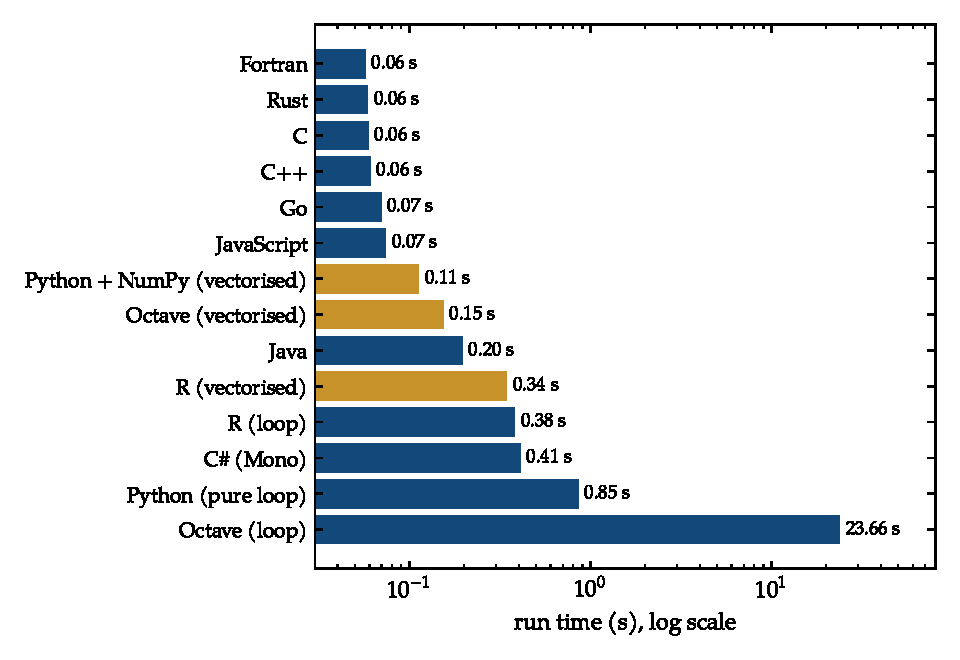
\includegraphics[width=0.85\linewidth]{figures/benchmark.pdf}
\caption{Time to evaluate the trapezoidal rule with $n = 10^7$ intervals (best of three
runs, one core of a 2.1~GHz Intel Xeon server, Linux). Blue bars: an explicit loop; gold bars: a
vectorised expression. Versions: GCC/gfortran 13.3 with \code{-O2}, OpenJDK 21, Node.js
22, Go 1.24, Rust 1.97, Mono 6.8, CPython 3.13 with NumPy 2.5, GNU Octave 8.4, R 4.3.
Note the logarithmic scale.}
\label{fig:benchmark}
\end{figure}

Several lessons can be read from the figure.
\begin{itemize}
\item \textbf{The compiled languages are all about equally fast.} C, C++, Fortran and Rust
  produce essentially the same machine code; Go is close behind. The run time is dominated
  by the $10^7$ calls to $\sin$.
\item \textbf{JIT compilation works.} JavaScript, a dynamic language, runs this loop
  within about 25\% of C, thanks to the V8 JIT compiler. Java is slower here mainly because
  its \code{Math.sin} guarantees a particular accuracy in software. The old Mono runtime is
  much slower than modern .NET would be.
\item \textbf{Interpreted loops are slow.} The pure-\py loop is about 15 times slower
  than C, and the Octave loop about 400 times slower. (MATLAB's JIT engine runs such loops
  much faster than Octave; the difference shows how much the implementation matters.)
\item \textbf{Vectorisation recovers most of the speed.} NumPy and vectorised Octave
  bring the interpreted languages to within a factor of 2--3 of C, at the cost of
  allocating arrays of $10^7$ numbers (80~MB each).
\item \textbf{R's loop is surprisingly fast} here because R compiles functions and loops
  to bytecode; its vectorised version is not faster in this case because creating the large
  arrays costs as much as the loop.
\end{itemize}
Two languages are missing or misrepresented in the figure. Julia was not installed on
the computer used for the timings, so it is not shown; a compiled Julia loop is expected to
run at about the speed of C, Fortran and Rust. And C\# was timed with the old Mono runtime,
not with current .NET, which runs such a loop much faster.

Benchmarks like this one measure one narrow thing on one computer. Real programs spend
their time in many different places, and a program that is a hundred times faster but
takes a week longer to write and test is often the worse choice. Measure before you
optimise --- and optimise the part that actually takes the time.

\section{Syntax at a glance}

Table~\ref{tab:syntax} collects the basic syntax of the main languages of these notes on
one page. Use it as a quick reference when reading unfamiliar code.

\begin{sidewaystable}
\centering
\caption{Basic syntax compared. ``Index'' is the first array index; ``Block'' is how a block
of code is delimited.}
\label{tab:syntax}
\small
\setlength{\tabcolsep}{3pt}
\resizebox{\linewidth}{!}{%
\begin{tabular}{@{}>{\bfseries}l>{\ttfamily}l>{\ttfamily}l>{\ttfamily}l>{\ttfamily}l>{\ttfamily}l@{}}
\toprule
 & \normalfont\bfseries Python & \normalfont\bfseries Fortran & \normalfont\bfseries C / C++ & \normalfont\bfseries Java / C\# & \normalfont\bfseries JavaScript\\
\midrule
Comment & \# text & ! text & // text & // text & // text\\
Variable & x = 1.0 & real(dp) :: x & double x = 1.0; & double x = 1.0; & let x = 1.0;\\
Constant & G = 9.81 & real, parameter :: & const double & final / const & const g = 9.81;\\
Power & x**2 & x**2 & pow(x, 2) & Math.pow(x, 2) & x ** 2\\
Int.\ division & 7 // 2 & 7 / 2 & 7 / 2 & 7 / 2 & Math.trunc(7/2)\\
Not equal & != & /= & != & != & !==\\
And / or & and, or & .and., .or. & \&\&, || & \&\&, || & \&\&, ||\\
Block & indentation & end ... & \{ \} & \{ \} & \{ \}\\
If & if x > 0: & if (x > 0) then & if (x > 0) \{ & if (x > 0) \{ & if (x > 0) \{\\
Loop & for i in range(n): & do i = 1, n & for (i=0; i<n; i++) & for (i=0; i<n; i++) & for (let i=0; i<n; i++)\\
Function & def f(x): & function f(x) & double f(double x) & static double f(double x) & function f(x) \{\\
Array & [1.0, 2.0] & [1.0, 2.0] & \{1.0, 2.0\} & \{1.0, 2.0\} & [1.0, 2.0]\\
Index & 0 & 1 (any) & 0 & 0 & 0\\
Length & len(a) & size(a) & (pass n) / a.size() & a.length / a.Length & a.length\\
Print & print(f"\{x:.3f\}") & print \textquotesingle{}(f0.3)\textquotesingle{}, x & printf("\%.3f", x) & printf / \$"\{x:F3\}" & x.toFixed(3)\\
\midrule
 & \normalfont\bfseries MATLAB & \normalfont\bfseries R & \normalfont\bfseries Julia & \normalfont\bfseries Wolfram & \normalfont\bfseries Rust\\
\midrule
Comment & \% text & \# text & \# text & (* text *) & // text\\
Variable & x = 1.0; & x <- 1.0 & x = 1.0 & x = 1.0 & let x = 1.0;\\
Constant & {\normalfont n/a} & {\normalfont n/a} & const g = 9.81 & {\normalfont n/a} & const G: f64 = 9.81;\\
Power & x\^{}2, x.\^{}2 & x\^{}2 & x\^{}2 & x\^{}2 & x.powi(2)\\
Int.\ division & idivide / floor & 7 \%/\% 2 & div(7, 2) & Quotient[7, 2] & 7 / 2\\
Not equal & \textasciitilde= & != & != & != & !=\\
And / or & \&\&, || & \&\&, || & \&\&, || & \&\&, || & \&\&, ||\\
Block & end & \{ \} & end & [ ] & \{ \}\\
If & if x > 0 & if (x > 0) \{ & if x > 0 & If[x > 0, ...] & if x > 0.0 \{\\
Loop & for i = 1:n & for (i in 1:n) \{ & for i in 1:n & Do[..., \{i, n\}] & for i in 0..n \{\\
Function & function y = f(x) & f <- function(x) & f(x) = ... & f[x\_] := ... & fn f(x: f64) -> f64\\
Array & [1.0 2.0] & c(1.0, 2.0) & [1.0, 2.0] & \{1.0, 2.0\} & vec![1.0, 2.0]\\
Index & 1 & 1 & 1 & 1 & 0\\
Length & numel(a) & length(a) & length(a) & Length[a] & a.len()\\
Print & fprintf(\textquotesingle{}\%.3f\textquotesingle{}, x) & sprintf("\%.3f", x) & @printf("\%.3f", x) & NumberForm[x, \{4,3\}] & println!("\{:.3\}", x)\\
\bottomrule
\end{tabular}}
\end{sidewaystable}

\begin{exercises}
\item Choose two languages from this chapter that you have not used before. Install them
  (or use an online compiler) and run their versions of the Rosetta program.
\item Add a fourth task to the \py program: solve the $3\times3$ linear system with
  \code{gauss\_solve}. Then add the same task to the C version.
\item Change the trapezoidal rule to Simpson's rule in three languages of your choice.
  Verify that the error for $n = 100$ drops to about $10^{-8}$.
\item Repeat the speed test on your own computer with \py (loop and NumPy) and one compiled
  language. Do you see the same ratios?
\item Add a Numba-compiled version of the trapezoidal loop (\code{from numba import njit})
  to the \py benchmark. How close does it come to C?
\item Find the Rosetta Code website (\url{https://rosettacode.org}) and look up a task of
  your choice, such as ``Matrix multiplication'' or ``Numerical integration''. Compare the
  solutions in three languages.
\end{exercises}

% =====================================================================
\BookChapter[Choosing a Language]{Choosing a Language and Writing Code Others Can Trust}
\label{ch:choosing}

\begin{researchquestion}
Which language should you use for a given task, and how do you make the result trustworthy?
\end{researchquestion}
% =====================================================================

You have now seen a dozen languages. This final chapter steps back and asks two practical
questions. Given an engineering task, which language should you use? And whatever the
language, how do you write code that you, your colleagues and your clients can trust?

\LearningOutcomes{Choose a language for a task by asking who will use the code, where it must run and how long it must live; learn a new language systematically; keep code under version control; test a calculation against known answers and limiting cases; document code so that results can be reproduced; and use AI coding assistants without giving up responsibility for the result.}

\section{Questions to ask before choosing}

There is no best language, only a best language \emph{for a given task, team and
situation}. The following questions usually decide the matter.

\begin{enumerate}
\item \textbf{What already exists?} If your company's simulation tool is scripted in \py,
  or your laboratory's instruments come with a LabVIEW driver, or your supervisor's
  solver is in Fortran, that is usually the strongest argument. Reusing tested code beats
  writing new code.
\item \textbf{Who will use and maintain it?} Code outlives its author's interest in it. A
  \py script can be read by most engineers; a clever C++ template library may be readable
  only by you. Write for the person who will inherit your code.
\item \textbf{Where must it run?} A web page needs JavaScript. A microcontroller needs C,
  C++ or Rust. A PLC needs IEC 61131-3 languages. A cluster job can use almost anything,
  but Fortran, C++ and \py dominate. A colleague without a MATLAB licence cannot run your
  MATLAB code.
\item \textbf{How fast must it be?} Most engineering scripts run in seconds, and speed
  does not matter. If it does, first find out \emph{where} the time is spent (profiling),
  then vectorise, use a library, or move the hot loop into a compiled language
  (Figure~\ref{fig:benchmark}).
\item \textbf{How safe must it be?} Software that controls a vehicle, a medical device or
  a chemical plant is subject to standards (ISO 26262, IEC 62304, IEC 61508) that restrict
  languages and require rigorous verification. There, C with MISRA rules, Ada/SPARK, Rust,
  certified code generators (Simulink, SCADE) and PLC languages are typical.
\item \textbf{What libraries do you need?} Statistics: R or \py. Machine learning: \py.
  Control design: MATLAB or \py. Differential equations at scale: Julia, \py, C++ or
  Fortran. Symbolic derivations: Wolfram, SymPy or Maple.
\item \textbf{How long will it live?} A throw-away analysis can be a notebook. A tool used
  by a hundred people for ten years needs a language with a stable future, tests,
  documentation and version control.
\end{enumerate}

\section{A rough decision guide}

Table~\ref{tab:ch16:guide} gives a first suggestion for some common tasks. Treat it as a
starting point for the questions above, not as a rule.

\begin{table}[htbp]
\centering\small
\caption[{A rough decision guide}]{A rough decision guide. The right-hand column names the
languages to consider first; local habits and existing code often decide otherwise.}
\label{tab:ch16:guide}
\begin{tabularx}{\linewidth}{@{}>{\raggedright\arraybackslash}p{5.6cm}>{\raggedright\arraybackslash}X@{}}
\toprule
\textbf{If you need to \ldots} & \textbf{consider first \ldots}\\
\midrule
analyse data, automate a task, prototype a model, drive other software & \py\\
do statistics, designed experiments, reliability analysis & R (or \py)\\
design control systems, process signals, model-based design & MATLAB/Simulink (or \py)\\
derive formulas, solve equations symbolically & Wolfram Language, SymPy, Maple\\
write a fast numerical solver from scratch & Julia, modern Fortran, C++\\
extend an existing large simulation code & the language it is written in\\
program a microcontroller or write firmware & C, C++, Rust\\
program an industrial controller (PLC) & Structured Text, Ladder Diagram\\
design digital hardware & VHDL, Verilog\\
build an interactive web tool or dashboard & JavaScript/TypeScript (or \py with Streamlit/Dash, R with Shiny)\\
build a Windows desktop application or a CAD plug-in & C\#\\
build an Android or iOS app & Kotlin, Swift\\
query or manage a database & SQL\\
automate a cluster workflow & Bash (plus \py)\\
model a multi-domain physical system & Modelica, Simscape, ModelingToolkit\\
\bottomrule
\end{tabularx}
\end{table}

\section{How to learn a new language quickly}

Sooner or later you will need a language you do not know. A systematic approach:
\begin{enumerate}
\item \textbf{Get ``Hello, world'' running.} Install the tools and learn the
  edit--run cycle. This is often the hardest step.
\item \textbf{Map the core features} using the checklist from Chapter~\ref{ch:intro}:
  types, variables, operators, \code{if}, loops, functions, arrays, I/O, modules, errors.
  Table~\ref{tab:syntax} and the reference guides at the back help.
\item \textbf{Translate a program you already understand}, such as the drag or Rosetta
  programs of these notes. Because you know what the output must be, every difference
  teaches you something.
\item \textbf{Read idiomatic code} --- the standard library, well-known packages, the
  official tutorial --- to learn how experienced users write the language, not just what
  compiles.
\item \textbf{Learn the tools}: the package manager, the debugger, the test framework, the
  formatter.
\end{enumerate}

\section{Version control with Git}

\term[version control]{Version control} records every change to a set of files, who made it and why, and
lets you go back to any earlier state. It is essential for code, and useful for any text
files (\LaTeX\ reports, data-processing scripts, configuration). \textbf{Git} is the
standard tool; \textbf{GitHub}, \textbf{GitLab} and similar services host Git
repositories online and support collaboration.
\begin{lstlisting}[style=shell]
$ git init                         # start tracking the current folder
$ git add drag.py                  # stage a file for the next snapshot
$ git commit -m "Euler solver for drag problem"   # record the snapshot
$ git log --oneline                # list the history
$ git diff                         # what changed since the last commit?
$ git checkout -b smaller-dt       # create a branch to try an idea
$ git push origin main             # upload to GitHub/GitLab
\end{lstlisting}
Commit often, with messages that explain \emph{why} something changed. Never commit
passwords or large generated data files. Graphical tools such as GitHub Desktop and the Git
support built into VS Code make all of this easier.

\section{Testing}

A calculation you have not checked is a guess. Chapter~\ref{ch:python} introduced
automated tests; here are the kinds of checks engineers should build into their programs,
in any language:
\begin{itemize}
\item \textbf{Known solutions}: compare with an exact solution (as we did with
  $\tanh$), a textbook example, or a hand calculation.
\item \textbf{Limiting cases}: with zero drag the speed must be $gt$; with zero load the
  deflection must be zero.
\item \textbf{Conservation laws and symmetries}: energy in the MD simulation, mass and
  energy balances in process models, symmetric stiffness matrices.
\item \textbf{Convergence}: halving the time step or refining the mesh should change the
  result by the amount the method's order predicts.
\item \textbf{Units and dimensions}: check every formula; use unit-aware libraries where
  possible.
\item \textbf{Independent implementation}: as in Chapter~\ref{ch:rosetta}, a second
  implementation in another language or by another person catches errors that a single
  author does not see.
\item \textbf{Regression tests}: once a result is verified, store it and check that future
  versions of the code still reproduce it.
\end{itemize}
Every language has test frameworks: \code{pytest} (\py), \code{testthat} (R), MATLAB's
\code{matlab.unittest}, JUnit (Java), xUnit/NUnit (C\#), GoogleTest and Catch2 (C++),
\code{pFUnit} and \code{test-drive} (Fortran), Julia's \code{Test}, Rust's built-in
\code{cargo test}, and Jest or Vitest (JavaScript).

\section{Documentation and reproducibility}

Good engineering code is \emph{documented}: every function says what it does, what its
inputs and outputs are, and \emph{in which units}; a README file explains how to install
and run the program; and assumptions and limitations are written down. Good engineering
results are \emph{reproducible}: someone else, or you next year, can regenerate every
number and figure from the raw data and the code. That requires recording the versions of
the language and of every package (\file{requirements.txt}, \file{environment.yml},
\file{renv.lock}, \file{Project.toml}, \file{Cargo.lock}), fixing random seeds, and keeping
code, data and results under version control. Publishing code and data alongside a report
or paper, in a public repository with a clear licence, is increasingly expected.

\section{AI coding assistants}
\label{sec:ai-assistants}

Since about 2022, AI assistants based on large language models have become part of
everyday programming. They can explain unfamiliar code, translate a program from MATLAB to
\py, write a first version of a function from a description, suggest tests, and find bugs.
They know every language in these notes. Used well, they make you much more productive and
are an excellent tutor for learning a new language.

They can also be confidently wrong. An assistant may invent a function that does not
exist, use a formula with a wrong constant, mix up 0- and 1-based indices when translating,
or produce code that runs and gives a plausible but incorrect answer --- the most dangerous
kind of error (Chapter~\ref{ch:howcoderuns}). The engineering responsibility for a result
remains with the engineer who signs it. Some rules for using AI assistants:
\begin{enumerate}
\item \textbf{Understand every line} you use. If you could not explain it to a colleague,
  you cannot vouch for it. This is why reading code in many languages --- the purpose of
  these notes --- matters more, not less, in the age of AI.
\item \textbf{Test generated code} with the same checks as your own: known solutions,
  limiting cases, units.
\item \textbf{Give precise specifications}: inputs, outputs, units, the method to use, and
  an example with the expected answer.
\item \textbf{Follow your course and employer rules} on what may be shared with external
  services (confidential data, proprietary code) and on how AI use must be acknowledged in
  assessed work.
\end{enumerate}

\section{Software licences}

When you use or share code, its \term{licence} decides what you may do with it. Open-source
licences fall into two broad groups. \emph{Permissive} licences (MIT, BSD, Apache 2.0) allow
almost any use, including in commercial products, provided the copyright notice is kept.
\emph{Copyleft} licences (GPL, LGPL) require that modified versions you distribute are
released under the same licence. Data and documents are often shared under Creative Commons
licences (CC BY 4.0, for example, requires attribution). Commercial software (MATLAB,
Mathematica, many simulation packages) comes with licence terms that may restrict who can
run it and for what purpose. Check before you build on someone else's code.

\section{A last word}

Choosing a language is an engineering decision, and it deserves the same care as choosing
a material or a safety factor. Learn \py well, learn to read the others, and check what
you compute. The Epilogue that follows looks at where these languages came from and
where they may be going.

\begin{exercises}
\item For each of the following tasks, choose a language and justify your choice in two or
  three sentences: (a) logging and plotting data from a temperature sensor on a Raspberry
  Pi; (b) a cost estimate that the finance department will check; (c) a controller for a
  conveyor belt; (d) a 3D simulation of airflow around a building on a cluster; (e) an
  interactive web page that lets clients size a heat exchanger; (f) a statistical analysis
  of fatigue-test results.
\item Create a GitHub repository for your ENG 101 code. Add a README that explains how to
  run each program, a \file{requirements.txt}, and a test for at least one function.
\item Ask an AI assistant to translate \file{drag.m} into \py. Check the translation line
  by line. Did it handle the indices and the time vector correctly? Did it produce the
  same table?
\item Write a test that checks the convergence order of the Euler method for the drag
  problem: the error at $t = 6\unit{s}$ should halve when $\Delta t$ is halved.
\item Read the licence of NumPy and of one commercial program you use. What may you do
  with each, and what may you not?
\end{exercises}

\ProjectChapter{Epilogue: The Past and Future of the Languages of Engineering}{epilogue}
\index{history of programming languages}\index{future of programming}

\begin{researchquestion}
Where did the languages of engineering come from, how do they change, and what will an
engineer's programming look like when you graduate?
\end{researchquestion}

In 1957 an engineer who wanted a computer to evaluate a formula had to translate it by
hand into hundreds of machine instructions. The first Fortran compiler did that
translation automatically, and its name said so: \emph{formula translation}. Today you can
type a differential equation into a notebook and receive its exact solution, or describe a
calculation in plain English and receive a draft program in any language of these notes.
The title of these notes, \emph{From Formulas to Programs}, describes a road that
engineers have been shortening for seventy years. This epilogue looks back along that
road, draws out the patterns, and then looks ahead. The look ahead is opinion, not fact;
read it as one engineer's informed guess.

\section*{Every language began as somebody's problem}

None of the languages in these notes was designed to be a ``language of engineering''.
Each was built by people who were stuck. John Backus was tired of hand-writing machine
code for formulas. Dennis Ritchie needed an operating system that could move from one
computer to another. Cleve Moler wanted his students to use good matrix software without
first learning Fortran. Guido van Rossum wanted a language that was pleasant to read. The
creators of Julia were tired of writing every program twice, once to try the idea and
once to make it fast. The table below lists these turning points.

\begin{table}[H]
\centering\small
\caption*{\textbf{\sffamily Six turning points.} Each new language answered a problem
that the languages of its time handled badly, and each answer is still in use.}
\begin{tabularx}{\textwidth}{@{}>{\RaggedRight\arraybackslash}p{0.11\textwidth}>{\RaggedRight\arraybackslash}p{0.38\textwidth}X@{}}
\toprule
\textbf{Years} & \textbf{The problem} & \textbf{The answer}\\
\midrule
1950s & Writing machine code for formulas is slow and full of errors. & Fortran: the computer translates the formula.\\\addlinespace
1970s & Software is tied to one model of computer. & C: one source code, compiled for any machine.\\\addlinespace
1980s & Engineers want matrices and plots without writing a compiled program. & MATLAB, and later the Wolfram Language: interactive computing in the notation of mathematics.\\\addlinespace
1980s--1990s & Programs grow to millions of lines and become impossible to organise. & C++, Java and C\#: objects, libraries and safer memory.\\\addlinespace
1990s--2000s & Scientists spend more time writing code than thinking about the problem. & \py and R: readable, free, and with a library for almost everything.\\\addlinespace
2010s & Fast code and convenient code are written in different languages; memory errors cause most security failures. & Julia: speed without a second language. Rust: safety without loss of speed.\\
\bottomrule
\end{tabularx}
\end{table}

The lesson for you is practical. A language is a tool that carries the experience of the
people who built it. When a language seems strange, ask what problem its designers had.
Fortran's arrays, C's pointers, MATLAB's matrices and \py's indentation all stop looking
arbitrary once you know the answer.

\section*{Four patterns in how languages change}

\subsection*{Languages rarely die; they settle into the foundations}

Fortran is almost seventy years old and still runs weather forecasts. C is over fifty and
still runs inside nearly every device you own. New languages do not replace old ones. They
are built on top of them. When you call NumPy to solve a linear system, \py hands the work
to C, which hands it to routines first written in Fortran. The old languages have moved
down into the foundations, where few people see them and everybody depends on them. This
is why an engineer who can \emph{read} an old language is valuable: the foundations
still need inspection and repair.

\subsection*{Each generation moves the programmer closer to the problem}

Machine code describes what the processor does. Fortran and C describe a calculation.
MATLAB and NumPy describe operations on whole matrices. The Wolfram Language and SymPy
work with the formula itself. Modelica lets you write the physical equations and leaves
the solution method to the tool. At every step the programmer writes less about the
\emph{machine} and more about the \emph{problem}, and a translator of some kind fills in
the rest. The history of programming languages is largely the history of better
translators.

\subsection*{Good ideas travel from one language to the next}

Array operations started in APL in the 1960s, became popular through MATLAB, and are now
in Fortran, \py, R and Julia. Objects started in Simula as a way to simulate queues and
traffic, and are now almost everywhere. Garbage collection came from Lisp, notebooks from
Mathematica, the data frame from S and R, and \code{async}/\code{await} became widespread through C\#.
Languages borrow freely, so the major languages grow more alike with time. This is good
news for a learner: an idea you understand in \py will meet you again, with different
spelling, in the next language you learn.

\subsection*{The community decides more than the syntax does}

\py is not the fastest language in these notes, nor the most elegant. It leads because of
what surrounds it: free libraries for nearly every task, teaching material at every
level, and millions of people who can answer a question. MATLAB holds its place through
its toolboxes and Simulink, R through its statistical packages, C through fifty years of
compilers for every chip. When you choose a language, you choose its libraries, its
tools and its people. That part of a language changes slowly, which is why the popularity
tables of Chapter~\ref{ch:intro} change slowly too.

\section*{The machine keeps changing under the languages}

For about forty years, programs became faster every year without anyone changing them,
because each new processor was faster than the last. Around 2005 that stopped. Since then
computers have gained more cores, not faster ones, and much of the fastest computing has
moved to graphics processors (GPUs) that perform thousands of simple operations at once.

This shift is reshaping the languages. A loop written the 1990s way uses one core of a
machine that has dozens. Languages and libraries that can spread work over many cores and
onto GPUs have gained ground: array libraries, Julia, the machine-learning frameworks
driven from \py, and newer additions to Fortran and C++. Even \py itself is changing: its
recent versions can be built without the internal lock that for thirty years prevented
two threads from running \py code at the same time. Expect this trend to continue. The
engineer of the next decade will more often describe \emph{what} should be computed for
a whole array or a whole grid, and leave it to the tools to decide \emph{where} it runs.

A second pressure is safety. A large share of serious security failures in software come
from memory errors that C and C++ allow (Chapter~\ref{ch:c}). As software takes control of
cars, medical devices and power grids, such errors become engineering hazards. Languages
that prevent them, with Rust as the leading example for low-level work, are being
adopted for new systems, and safety standards are likely to ask for them more often. The
existing C and C++ code will not disappear, but less new code of that kind will be
written by hand.

\section*{An old argument, open again}

The largest change of your student years is the AI assistant that writes code from a
description in ordinary words (Chapter~\ref{ch:choosing}). It has reopened an argument
that is almost fifty years old, and you should know both sides of it.

\subsection*{One view: the next programming language is the one you already speak}

Andrej Karpathy, a well-known AI researcher, summed up the new situation in one line:
``The hottest new programming language is English.'' In his account, software has passed
through three stages: programs written by hand, neural networks trained on data, and now
language models steered by instructions in everyday language. Jensen Huang, the head of
the chip maker Nvidia, drew a bolder conclusion at a summit in Dubai in 2024. For years,
he said, everyone had been told that children must learn to program; in his view the goal
of computing is the opposite, to make programming unnecessary, so that ``everybody in the
world is now a programmer.'' He advised young people to put their effort into knowing a
field well: biology, manufacturing, farming, education.

There is truth in this. People who have never written a loop can now produce a working
program by describing what they want. The barrier of syntax, which stopped many
beginners, is much lower than it was.

\subsection*{The other view: precise notation is a privilege, not a burden}

In the late 1970s the Dutch computer scientist Edsger Dijkstra wrote a short note with
the title \emph{On the foolishness of ``natural language programming''}. People were
already wishing that computers could be instructed in plain English. Dijkstra argued that
the wish was mistaken. Mathematics, he pointed out, made its great advances only after it
stopped being written in words and adopted symbols. We should, he wrote, ``regard the
convenience of using them as a privilege'': with symbols, a school pupil can do
calculations that once needed a genius. Everyday language feels easy, he added, mostly
because it lets us say things that are wrong or meaningless without noticing.

This matters to engineers in a direct way. The title of these notes begins with the word
\emph{formulas}, and a formula is exactly what Dijkstra was defending: a short statement
that means one thing. ``The drag grows with speed'' is a sentence. $F = c v^2$ is a
formula; it tells you by how much, and it can be checked. No engineering standard, drawing
or contract is written in loose prose where a number or a symbol can be used.

\subsection*{Both sides are partly right}

The two views are less opposed than they sound. Plain language is a good way to
\emph{start}: to say roughly what is wanted and get a first draft. Precise notation is
the only way to \emph{finish}: to state exactly what the program must do and to confirm
that it does. Seen against seventy years of history, the AI assistant is the next
translator in the line, from machine code to formulas, from formulas to matrices, from
matrices to equations, and now from sentences to programs. Earlier translators did not
make programmers unnecessary. Fortran did not remove the need to understand the formula;
it removed the need to count memory addresses.

There is one difference from the earlier translators, and it is important. A compiler is
built to translate the same input the same way every time, and when it fails it usually
says so. An AI assistant can produce a different program each time it is asked, and it
can be wrong while sounding certain. That is why the checking skills of these notes
matter more now, not less.

\section*{Where the road may lead}

\subsection*{Writing the code was never the hard part}

When Huang's remark spread, many working programmers gave the same reply: typing the
program was never the difficult part of the job. The difficult part was, and is,
deciding exactly what the program should do. Which cases must it handle? In which units?
To what accuracy? What should happen when the input is wrong? An assistant that types
quickly does not answer these questions. If they are left open, it fills the gaps with
its own guesses, and it does so quickly and with confidence.

For this reason many software teams now describe their work differently. They treat the
\emph{specification}, a careful written statement of what must be built, what must not,
and how to verify the result, as the thing that lasts. The code becomes something that
can be generated again whenever needed. Some call the human's new role ``architect and
reviewer'' in place of ``typist''. These are opinions from practitioners, not settled
findings, but engineers will recognise the idea at once. A bridge is built from drawings,
standards and test protocols, not from a conversation. The drawing is the lasting
record; the concrete is poured to match it.

\subsection*{Strict languages and tests become the safety net}

If a machine writes the program, something else must catch its mistakes. Two tools do
this well. The first is a strict language. A compiler for Fortran, C++ or Rust refuses a
program in which the types do not match, and so do the type checkers for \py
(Chapter~\ref{ch:python}). Some observers expect such languages to gain ground for this
reason: a generated program that must pass a strict checker is easier to trust than one
that merely runs. The second tool is the test. A set of cases with known answers, written
by a person who understands the problem, says precisely what ``correct'' means. In the
future an engineer may write the tests and leave much of the program to the machine. The
habit you are building in ENG~101, checking a result against an exact solution or a
limiting case, is exactly the skill this requires.

\subsection*{Engineering has been here before}

Electronics offers an encouraging precedent. Fifty years ago engineers drew every
transistor of a chip by hand. Today design software places billions of them
automatically. Electrical engineering did not disappear, and students of the subject
still learn how a circuit works and how to draw one. They need that knowledge to tell the
software what to build and to judge what it produces. The work moved to a higher level;
the understanding underneath stayed necessary. Programming is likely to follow the same
path.

\subsection*{Programs that can be differentiated, and models that learn}

Engineers have always needed derivatives: for optimisation, for sensitivity analysis, for
fitting models to data. A growing family of tools can differentiate an entire program
automatically, however long it is. This \emph{automatic differentiation} is what trains
neural networks, and it is spreading into simulation codes. It allows a simulation to be
tuned against measurements, and physical laws to be combined with models learned from
data. Languages and libraries built with this in mind, such as JAX and PyTorch in \py and
much of the Julia ecosystem, are likely to matter more in engineering computation.

\subsection*{Describing the system and letting the tool write the program}

In Simulink, an engineer draws a controller and a code generator writes the C program
that runs in the car. In Modelica, an engineer writes the equations of a pump and a pipe
and the tool derives the simulation. This style, in which the engineer works with a model
of the system and software produces the program, has been growing for thirty years. With
better tools and with AI assistance it will probably grow faster. More engineers will
work with models, and fewer will type every line.

\subsection*{What will probably not change}

Predictions about technology are often wrong, so it is worth listing what has stayed the
same since 1957 and is likely to stay the same.

\begin{itemize}
\item \textbf{The algorithm comes first.} A clear statement of the steps is still the
  hard part. No language and no assistant can supply it if you cannot say what you want.
\item \textbf{Numbers in a computer are approximate.} Rounding, overflow and cancellation
  (Chapter~\ref{ch:howcoderuns}) follow from how numbers are stored, not from the language.
\item \textbf{Units and assumptions live outside the code.} The Mars Climate Orbiter was
  lost through a mismatch of units that no compiler detected. The engineer still has to
  know what each number means.
\item \textbf{An unchecked result is a guess.} This holds whether the program was written
  by you, by a colleague, by a vendor or by a machine.
\item \textbf{Responsibility stays with a person.} The engineer who signs the design
  answers for the calculation behind it.
\end{itemize}

\begin{keyidea}[Key idea: learn the ideas, and the languages will follow]
Languages come and go on a timescale of decades; the ideas beneath them last much
longer. Variables, loops, functions, arrays, types, tests and the limits of
floating-point arithmetic were needed in 1957 and are needed now. If you learn those
ideas well in \py, each new language costs you a few days of syntax, not a new
education.
\end{keyidea}

\section*{What this means for you}

You will graduate into a profession in which programming is as ordinary as drawing or
report writing, and in which much routine code is drafted by machines. Three habits will
serve you whatever the languages of that time turn out to be.

Should you still learn to program, if a machine can write the code? Consider reading and
writing. Few people become novelists, and nobody suggests that the rest should stay
illiterate. Few people become mathematicians, yet every engineer learns calculus,
because without it you cannot tell whether a result makes sense. Programming is becoming
a literacy of the same kind. You learn it in order to think clearly about calculations
and to judge the ones that are handed to you.

\textbf{Learn one language deeply.} For you that language is \py. Depth in one language
teaches the ideas that transfer to the rest, and it gives you a place to test your
understanding.

\textbf{Read widely.} Use these notes to become comfortable opening a Fortran, C or
MATLAB file and working out what it does. The engineer who can read the old solver, the
vendor's script and the assistant's draft can judge all three.

\textbf{Check everything that matters.} Keep asking the question that runs through these
notes: \emph{how do I know this answer is right?} The tools for answering it, an exact
solution, a limiting case, a conservation law, a second method, do not depend on any
language.

Backus's team set out to let engineers write formulas and leave the machine instructions
to the computer. Seventy years later the computer can take on far more of the writing.
What it cannot take on is knowing which formula describes the problem, and whether the
result can be trusted. That part of the work was the engineer's in 1957, and it still is.

\section*{Sources for the debate}
{\small
A.~Karpathy, ``Software Is Changing (Again)'', talk at the Y~Combinator AI Startup School,
2025; the remark about English dates from an earlier post of his.
J.~Huang, remarks at the World Government Summit, Dubai, 2024, as reported in the
technology press.
E.~W.~Dijkstra, \emph{On the foolishness of ``natural language programming''}, note
EWD~667, \url{https://www.cs.utexas.edu/~EWD/transcriptions/EWD06xx/EWD667.html}.
The views on specifications, reviewing and strict languages are drawn from practitioner
essays published in 2025 and 2026 and are opinions, not established results.\par}

\backmatter
% =====================================================================
\ProjectChapter{Installing and Running the Languages}{app:install}
\setcounter{table}{0}\renewcommand{\thetable}{R\arabic{table}}
% =====================================================================

All languages in these notes except MATLAB and the full Mathematica can be installed for
free on Windows, macOS and Linux. Table~\ref{tab:install} lists the recommended tools. On
Windows, the \textbf{Windows Subsystem for Linux} (WSL) gives you a complete Ubuntu Linux
environment in which every Linux command in these notes works unchanged; install it with
\code{wsl --install} in an administrator PowerShell. On macOS, the package manager
\textbf{Homebrew} (\url{https://brew.sh}) installs most tools with one command.

\begin{table}[htbp]
\centering
\caption{Getting each language. ``Online'' lists a way to try the language in a web browser
without installing anything.}
\label{tab:install}
\small
\begin{tabularx}{\linewidth}{@{}l>{\RaggedRight\arraybackslash}X>{\RaggedRight\arraybackslash\ttfamily}p{3.9cm}>{\RaggedRight\arraybackslash}p{3.0cm}@{}}
\toprule
\textbf{Language} & \textbf{Install} & \normalfont\textbf{Ubuntu / WSL} & \textbf{Online}\\
\midrule
\py & Anaconda / Miniforge, python.org, uv & sudo apt install python3-pip & Google Colab, JupyterLite\\
Fortran & gfortran (GCC), Intel oneAPI ifx, LFortran & sudo apt install gfortran & godbolt.org, play.fortran-lang.org\\
C, C++ & GCC, Clang, Visual Studio (Windows), Xcode tools (macOS) & sudo apt install\newline build-essential & godbolt.org\\
C\# & .NET SDK (dotnet.microsoft.com) & sudo apt install dotnet-sdk-8.0 & dotnetfiddle.net\\
Java & Eclipse Temurin JDK (adoptium.net) & sudo apt install default-jdk & JDoodle, OneCompiler\\
JavaScript & any web browser; Node.js (nodejs.org) & sudo apt install nodejs & browser console\\
MATLAB & university licence (mathworks.com) & {\normalfont n/a} & MATLAB Online\\
Octave & octave.org & sudo apt install octave & octave-online.net\\
Wolfram & Mathematica (licence) or free Wolfram Engine & {\normalfont n/a} & Wolfram Cloud, Wolfram|Alpha\\
R & cran.r-project.org + RStudio/Positron & sudo apt install r-base & posit.cloud, webR\\
Julia & juliaup (julialang.org) & see julialang.org & JuliaHub\\
Rust & rustup (rustup.rs) & see rustup.rs & play.rust-lang.org\\
Go & go.dev/dl & sudo apt install golang & go.dev/play\\
SQL (SQLite) & sqlite.org; built into \py & sudo apt install sqlite3 & sqliteonline.com\\
Modelica & OpenModelica (openmodelica.org) & see website & n/a\\
\bottomrule
\end{tabularx}
\end{table}

\section*{One editor for everything}

\textbf{Visual Studio Code} (\url{https://code.visualstudio.com}) is a free editor that
supports every language in these notes through extensions: syntax highlighting, code
completion, running and debugging, Jupyter notebooks, Git integration and remote work on
WSL or a cluster. Install the extensions for \py, C/C++, Fortran (``Modern Fortran''), C\#,
Java, Julia, R, Rust (``rust-analyzer'') and Go as you need them.

\section*{Running the example programs}

All example programs of these notes are in the folder \file{code/} of the repository,
one sub-folder per language, together with the data files in \file{code/data/}. The
commands used to compile and run the drag program in each language were:
\begin{lstlisting}[style=shell]
$ python3 drag.py                                 # Python
$ gfortran -O2 -Wall -o drag drag.f90 && ./drag   # Fortran
$ gcc -std=c11 -O2 -Wall -o drag drag.c -lm && ./drag     # C
$ g++ -std=c++20 -O2 -Wall -o drag drag.cpp && ./drag     # C++
$ mcs Drag.cs && mono Drag.exe                    # C# with Mono
$ dotnet run Drag.cs                              # C# with .NET 10 or later
$ java Drag.java                                  # Java 11 or later
$ node drag.js                                    # JavaScript
$ octave --eval drag                              # Octave; in MATLAB type: drag
$ Rscript drag.R                                  # R
$ julia drag.jl                                   # Julia
$ rustc -O drag.rs && ./drag                      # Rust
$ go run drag.go                                  # Go
$ wolframscript -file drag.wl                     # Wolfram Language
\end{lstlisting}
The programs that read a data file look for it in the folder \file{code/data/}. In the
programs this folder is written as \file{../data/}, so run each program from inside its
own language folder. The programs of Chapter~\ref{ch:rosetta} are the exception: they read
\file{yield.txt} from the current folder, and a copy of that file is kept in
\file{code/rosetta/} for this purpose.

To re-run every example at once and compare each output with the one printed in these
notes, run the checking script from the top folder of the repository. Languages that are
not installed on your computer are skipped.
\begin{lstlisting}[style=shell]
$ python3 tools/check_examples.py
\end{lstlisting}

% =====================================================================
\ProjectChapter{Python Quick Reference}{app:pyref}
% =====================================================================

\section*{Basics}
\begin{lstlisting}[language=Python]
x = 3.0; n = 10; name = "steel"; ok = True; nothing = None
type(x); int("3"); float("2.5"); str(42); round(3.14159, 2)
7 / 2   # 3.5      7 // 2  # 3      7 % 2  # 1      2 ** 10  # 1024
a == b; a != b; a < b <= c; x and y; x or y; not x
print(f"{x:8.3f} {n:5d} {x:.2e} {name:>10s}")
value = input("Prompt: ")          # always a string
\end{lstlisting}

\section*{Control flow}
\begin{lstlisting}[language=Python]
if x > 0:
    ...
elif x == 0:
    ...
else:
    ...
for i in range(n):          # 0 ... n-1
for i in range(1, n + 1):   # 1 ... n
for item in items:
for i, item in enumerate(items):
for a, b in zip(list_a, list_b):
while condition:
break; continue; pass
result = "big" if x > 10 else "small"      # conditional expression
\end{lstlisting}

\section*{Collections}
\begin{lstlisting}[language=Python]
L = [1, 2, 3]; L.append(4); L.insert(0, 0); L.pop(); L.sort(); len(L)
L[0]; L[-1]; L[1:3]; L[::-1]; 3 in L
squares = [x**2 for x in range(10) if x % 2 == 0]
t = (1, 2); a, b = t
d = {"steel": 7850}; d["al"] = 2700; d.get("ti", 0); d.keys(); d.items()
s = {1, 2, 3}; s.add(4); s & {2, 5}; s | {9}
\end{lstlisting}

\section*{Functions, classes, errors, files}
\begin{lstlisting}[language=Python]
def f(x, y=1.0, *args, **kwargs):
    """Docstring."""
    return x + y
g = lambda x: x**2

class Tank:
    def __init__(self, volume):
        self.volume = volume
    def mass(self, rho):
        return rho * self.volume

try:
    risky()
except (ValueError, ZeroDivisionError) as err:
    print("error:", err)
finally:
    cleanup()
raise ValueError("message"); assert x > 0, "x must be positive"

with open("data.txt") as f:            # "w" write, "a" append
    for line in f:
        values = [float(v) for v in line.split()]
\end{lstlisting}

\section*{NumPy, Matplotlib and SciPy}
\begin{lstlisting}[language=Python]
import numpy as np, matplotlib.pyplot as plt
a = np.array([1., 2., 3.]); np.zeros((3, 3)); np.ones(5); np.eye(3)
np.arange(0, 1, 0.1); np.linspace(0, 1, 11); np.random.default_rng(0).normal(size=5)
a.shape; a.reshape(3, 1); a.T; a[a > 1]; A[1, :]; A[:, 0]
a.sum(); a.mean(); a.std(ddof=1); a.max(); np.argmax(a); np.cumsum(a)
np.sin(a); np.exp(a); np.sqrt(a); np.abs(a); np.isclose(a, b)
A @ B; np.linalg.solve(A, b); np.linalg.eig(A); np.linalg.norm(a)
np.loadtxt("f.txt"); np.savetxt("out.txt", a); np.genfromtxt("f.csv", delimiter=",")

fig, ax = plt.subplots()
ax.plot(x, y, "o-", label="data"); ax.set_xlabel("x (m)"); ax.legend()
fig.savefig("plot.pdf")

from scipy.optimize import brentq, fsolve, minimize, curve_fit
from scipy.integrate import quad, solve_ivp
from scipy.interpolate import interp1d
\end{lstlisting}

% =====================================================================
\ProjectChapter{Numerical Functions Across Languages}{app:functions}
% =====================================================================

\begin{sidewaystable}
\centering
\caption{Common mathematical and numerical operations.}
\small
\setlength{\tabcolsep}{3pt}
\resizebox{\linewidth}{!}{%
\begin{tabular}{@{}>{\bfseries}l>{\ttfamily}l>{\ttfamily}l>{\ttfamily}l>{\ttfamily}l>{\ttfamily}l@{}}
\toprule
 & \normalfont\bfseries \py & \normalfont\bfseries MATLAB & \normalfont\bfseries R & \normalfont\bfseries Julia & \normalfont\bfseries C / C++\\
\midrule
$\sqrt{x}$ & math.sqrt(x) & sqrt(x) & sqrt(x) & sqrt(x) & sqrt(x)\\
$e^x$, $\ln x$ & math.exp, math.log & exp, log & exp, log & exp, log & exp, log\\
$\log_{10} x$ & math.log10(x) & log10(x) & log10(x) & log10(x) & log10(x)\\
$|x|$ & abs(x) & abs(x) & abs(x) & abs(x) & fabs(x) / std::abs\\
$\pi$ & math.pi & pi & pi & pi, \textbackslash pi & M\_PI / std::numbers::pi\\
$\operatorname{atan2}(y,x)$ & math.atan2(y, x) & atan2(y, x) & atan2(y, x) & atan(y, x) & atan2(y, x)\\
round & round(x) & round(x) & round(x) & round(x) & round(x)\\
remainder & x \% y & mod(x, y) & x \%\% y & mod(x, y) & fmod(x, y)\\
sum & np.sum(a) & sum(a) & sum(a) & sum(a) & std::accumulate\\
mean, std & np.mean, np.std(ddof=1) & mean, std & mean, sd & mean, std & (by hand)\\
min, max & np.min, np.max & min, max & min, max & minimum, maximum & std::min\_element\\
sort & np.sort(a) & sort(a) & sort(a) & sort(a) & std::sort\\
cumulative sum & np.cumsum(a) & cumsum(a) & cumsum(a) & cumsum(a) & std::partial\_sum\\
dot product & a @ b & dot(a, b) & sum(a*b) & dot(a, b) & std::inner\_product\\
matrix product & A @ B & A*B & A \%*\% B & A*B & (Eigen) A*B\\
transpose & A.T & A\textquotesingle{} & t(A) & A\textquotesingle{} & (Eigen) A.transpose()\\
solve $A\mathbf{x}=\mathbf{b}$ & np.linalg.solve & A\textbackslash b & solve(A, b) & A\textbackslash b & (LAPACK / Eigen)\\
eigenvalues & np.linalg.eigvals & eig(A) & eigen(A) & eigvals(A) & (LAPACK / Eigen)\\
root of $f$ & scipy.optimize.brentq & fzero & uniroot & (Roots.jl) find\_zero & (GSL)\\
integral & scipy.integrate.quad & integral & integrate & (QuadGK.jl) quadgk & (GSL)\\
ODE & solve\_ivp & ode45 & deSolve::ode & (DiffEq.jl) solve & (Boost.Odeint)\\
interpolate & np.interp & interp1 & approx & (Interpolations.jl) & {\normalfont n/a}\\
polynomial fit & np.polyfit & polyfit & lm(y \textasciitilde\ poly(x, n)) & (Polynomials.jl) fit & {\normalfont n/a}\\
random uniform & rng.random() & rand & runif(1) & rand() & std::uniform\_real\_distribution\\
random normal & rng.normal() & randn & rnorm(1) & randn() & std::normal\_distribution\\
read table & np.loadtxt, pd.read\_csv & readmatrix, readtable & read.csv & CSV.read & (by hand)\\
\bottomrule
\end{tabular}}
\end{sidewaystable}

\noindent In C and C++, include \code{<math.h>}/\code{<cmath>} for the mathematical functions.
Fortran uses the same names as C for most intrinsics (\code{sqrt}, \code{exp}, \code{log},
\code{log10}, \code{abs}, \code{atan2}, \code{mod}) plus array intrinsics (\code{sum},
\code{maxval}, \code{matmul}, \code{dot\_product}, \code{transpose}).

% =====================================================================
\ProjectChapter{Glossary}{app:glossary}
% =====================================================================

\begin{description}[style=nextline,leftmargin=1.2em,font=\sffamily\bfseries]
\item[Algorithm] A finite, precise sequence of steps that solves a problem.
\item[API] Application programming interface: the set of functions, classes and
  conventions through which one piece of software is used by another.
\item[Array] An ordered collection of elements of the same type, accessed by index.
\item[Assembly language] A human-readable form of machine code, specific to one processor
  family.
\item[Broadcasting] Combining arrays of different shapes by automatically extending the
  smaller one (NumPy, Julia, MATLAB).
\item[Bug] An error in a program. \textbf{Debugging} is finding and fixing it.
\item[Bytecode] An intermediate, platform-independent code executed by a virtual machine
  or interpreter.
\item[Class] A blueprint for objects, defining their data and methods.
\item[Column-major] Storing a matrix column by column in memory (Fortran, MATLAB, R,
  Julia).
\item[Compiler] A program that translates source code into machine code (or bytecode)
  before the program runs.
\item[Debugger] A tool that lets you pause a running program, step through it and inspect
  variables.
\item[Dynamic typing] Types belong to values and are checked while the program runs.
\item[Exception] An object that signals a run-time error and can be caught and handled.
\item[Floating-point number] A computer representation of a real number with a limited
  number of significant digits (IEEE 754).
\item[Function] A named, reusable block of code with inputs (parameters) and usually an
  output (return value). Also called a procedure, subroutine or method.
\item[Garbage collector] Part of a language runtime that automatically frees memory that is
  no longer used.
\item[Heap] The memory region for data whose size or lifetime is decided at run time.
\item[IDE] Integrated development environment: editor, runner, debugger and other tools in
  one program.
\item[Immutable] Cannot be changed after creation (e.g.\ \py strings and tuples).
\item[Inheritance] Defining a new class as an extension of an existing one.
\item[Interpreter] A program that executes source code (or bytecode) directly, statement
  by statement.
\item[JIT compilation] Just-in-time compilation: translating code to machine code while
  the program runs, just before it is needed.
\item[Library] A collection of reusable, tested code (functions, classes) for a task.
\item[Linker] A program that combines compiled object files and libraries into an
  executable.
\item[Literal] A value written directly in the code, such as \code{3.14} or
  \code{"steel"}.
\item[Machine epsilon] The gap between 1 and the next larger floating-point number;
  $\approx 2.2\times10^{-16}$ in double precision.
\item[Memory leak] Memory that a program allocates but never frees.
\item[Method] A function that belongs to a class or object.
\item[Module] A file or unit of code that groups related definitions and can be imported.
\item[Multiple dispatch] Choosing which version of a function to run based on the types of
  all its arguments (Julia).
\item[Notebook] A document mixing executable code cells, results and text (Jupyter,
  Mathematica, MATLAB Live Scripts, Pluto).
\item[Object] A bundle of data and the methods that act on it; an instance of a class.
\item[Off-by-one error] A loop or index that is one step too short or too long.
\item[Operator overloading] Defining what operators such as \code{+} and \code{*} mean for
  user-defined types.
\item[Overflow] A result too large for the type that must hold it.
\item[Package manager] A tool that installs libraries and their dependencies (\code{pip},
  \code{conda}, CRAN, \code{npm}, Cargo, NuGet, Maven, Julia's Pkg).
\item[Paradigm] A style of programming: imperative, procedural, object-oriented,
  functional, declarative, array.
\item[Pointer] A variable holding a memory address (C, C++, Fortran pointers).
\item[Polymorphism] Code that works with objects of different types through a common
  interface.
\item[Profiling] Measuring where a program spends its time.
\item[Recursion] A function that calls itself.
\item[Reference] A name that refers to an object without copying it.
\item[REPL] Read--evaluate--print loop: an interactive prompt.
\item[Row-major] Storing a matrix row by row in memory (C, C++, \py/NumPy by default).
\item[Runtime] The period when a program runs; also the support software a language needs
  while running (JVM, .NET runtime).
\item[Scope] The region of a program in which a name is visible.
\item[Source code] The human-readable text of a program.
\item[Stack] The memory region holding the local variables of active function calls.
\item[Standard library] The library that comes with a language implementation.
\item[Static typing] Types are attached to variables and checked before the program runs.
\item[String] A sequence of characters (text).
\item[Syntax] The grammar rules of a language.
\item[Type] The kind of a value (integer, float, string, \ldots), which determines how it is
  stored and what can be done with it.
\item[Undefined behaviour] In C and C++, an operation whose result the language standard
  does not define (e.g.\ reading outside an array); anything may happen.
\item[Unicode, UTF-8] The universal character set and its most common byte encoding.
\item[Variable] A name that refers to a value stored in memory.
\item[Vectorisation] Expressing a computation as operations on whole arrays instead of
  explicit loops; also the use of SIMD processor instructions.
\item[Version control] Recording the history of changes to files (Git).
\item[Virtual machine] Software that executes bytecode (JVM, .NET CLR).
\end{description}


% =====================================================================
\ProjectChapter{Answers to Selected Exercises}{app:answers}
% =====================================================================

These answers are short on purpose. Try each exercise yourself before you read them. Where
a numerical answer is given, it was computed with the programs of these notes.

\section*{Chapter 1}
\begin{description}[style=nextline,leftmargin=0pt,font=\normalfont]
\item[\AnswerRef{1.1}] $(252, 105) \to (105, 42) \to (42, 21) \to (21, 0)$. The loop body runs three
  times and the greatest common divisor is 21.
\item[\AnswerRef{1.2}] (a) declarative (and functional): the formula states what to compute; (b)
  imperative; (c) declarative; (d) array programming; (e) object-oriented.
\item[\AnswerRef{1.4}] Compiled languages need a defined entry point because the operating system starts
  an executable file at one particular place; interpreters simply start at the top of the
  script.
\item[\AnswerRef{1.6}] If a value read from a form or a file is a string, \code{+} concatenates instead
  of adding, so a load of \code{"3"} kN plus 4 kN becomes \code{"34"}. No error is raised,
  and the wrong number propagates silently.
\end{description}

\section*{Chapter 2}
\begin{description}[style=nextline,leftmargin=0pt,font=\normalfont]
\item[\AnswerRef{2.1}] $5 = 101_2$, $12 = 1100_2$, $100 = 1100100_2$.
\item[\AnswerRef{2.2}] An unsigned 16-bit integer holds $0$ to $2^{16}-1 = 65\,535$. Counting once per
  second, it overflows after $65\,536\unit{s} \approx 18.2$ hours and starts again at 0.
\item[\AnswerRef{2.4}] The textbook formula gives $-7.45\times10^{-9}$, which is wrong in the first
  digit; the rewritten formula gives $-1.0000\times10^{-8}$, which is correct. In the textbook
  formula $-b + \sqrt{b^2 - 4ac}$ subtracts two numbers that agree in almost all digits.
\item[\AnswerRef{2.5}] With a single-precision running total, summing from $n=1$ upwards gives
  $1.6447253$, summing downwards gives $1.644933$, and $\pi^2/6 = 1.6449341$. Summing
  upwards, the small late terms are added to a large total and are lost below its last
  significant digit. Summing the small terms first lets them accumulate before they meet the
  large ones.
\item[\AnswerRef{2.6}] The result is \code{[[1, 0, 0], [1, 0, 0], [1, 0, 0]]}: the outer list contains
  three references to the \emph{same} inner list. Create independent rows with
  \code{a = [[0]*3 for \_ in range(3)]}, or use \code{numpy.zeros((3, 3))}.
\end{description}

\section*{Chapter 3 (Python)}
\begin{description}[style=nextline,leftmargin=0pt,font=\normalfont]
\item[\AnswerRef{3.2}] $-40$ is the same on both scales.
\item[\AnswerRef{3.3}] The maximum absolute errors over $0 \le t \le 20\unit{s}$ are:
\begin{center}
\small
\begin{tabular}{@{}lcccc@{}}
\toprule
$\Delta t$ (s) & 0.5 & 0.25 & 0.125 & 0.0625\\
max.\ error (m/s) & 0.928 & 0.458 & 0.227 & 0.113\\
\bottomrule
\end{tabular}
\end{center}
  Each halving of $\Delta t$ halves the error: the Euler method is first-order accurate.
\item[\AnswerRef{3.6}] For fully turbulent flow in a rough pipe the friction factor is nearly constant
  and $\Delta p \propto v^2 \propto Q^2$, so the log--log plot has a slope close to 2
  (slightly less at lower Reynolds numbers, where $f_D$ still decreases with $\mathrm{Re}$).
  If part of the range is laminar, the slope there is 1, because $\Delta p \propto Q$ in
  Poiseuille flow.
\item[\AnswerRef{3.8}] With $\Delta t = 0.02$ the total energy is no longer conserved: in
  our run it drifts from $0.63$ to $0.55$ over 2000 steps. With $\Delta t = 0.05$ two
  particles come so close in one step that the huge repulsive force throws them apart,
  the energy grows without limit, and after a few hundred steps the program prints
  \code{nan}. Nothing in the code reports an error. A time step must be small compared
  with the fastest motion in the system.
\end{description}

\section*{Chapter 4 (Fortran)}
\begin{description}[style=nextline,leftmargin=0pt,font=\normalfont]
\item[\AnswerRef{4.1}] The output changes only slightly: for example, the exact speed at $t = 6\unit{s}$
  becomes $43.8152$ instead of $43.8151$. The constant \code{0.25} is exactly representable
  in single precision, but \code{9.81} is stored as $9.8100004196\ldots$, an error of about
  $4\times10^{-8}$ relative. Such small, silent changes are exactly what makes this bug hard
  to find.
\item[\AnswerRef{4.5}] Under implicit typing \code{I} and \code{N} are integers; \code{X}, \code{S} and
  \code{RMS} are reals. Modern version: \code{rms = sqrt(sum(x(1:n)**2) / n)}.
\item[\AnswerRef{4.6}] The loop with the first index innermost is faster, because Fortran stores
  arrays by columns and this order reads memory contiguously.
\end{description}

\section*{Chapter 5 (C)}
\begin{description}[style=nextline,leftmargin=0pt,font=\normalfont]
\item[\AnswerRef{5.1}] The compiler itself succeeds, but the \emph{linker} reports undefined references
  to \code{sqrt} and \code{tanh}, because the maths library was not linked. (Some compilers
  replace simple calls by built-in instructions, so the error may not always appear.)
\item[\AnswerRef{5.2}] \code{7/2} is \code{3}; \code{7.0/2} is \code{3.5}; \code{7/2*2.0} is
  \code{6.0} (the integer division happens first); \code{(double)7/2} is \code{3.5};
  \code{-7/2} is \code{-3} (C truncates toward zero, unlike \py's \code{//}, which gives
  \code{-4}); \code{-7\%2} is \code{-1}.
\item[\AnswerRef{5.5}] Without \code{free}, the memory is released only when the program ends. In a
  function called repeatedly, or in a long-running program such as a controller, the leak
  grows until memory runs out.
\end{description}

\section*{Chapter 8 (Java)}
\begin{description}[style=nextline,leftmargin=0pt,font=\normalfont]
\item[\AnswerRef{8.2}] A heat loss of 50~W requires $R_\mathrm{total} = 45/50 = 0.9\unit{K/W}$. The
  other layers contribute $0.0542\unit{K/W}$, so the insulation must provide $0.8458\unit{K/W}$,
  i.e.\ $L = 0.8458 \times 0.035 \times 10 \approx 0.30\unit{m}$ of insulation.
\item[\AnswerRef{8.4}] \code{int} is a primitive value; \code{Integer} is an object that wraps one.
  Java's generic collections can hold only objects, so a list of integers is a
  \code{List<Integer>}.
\end{description}

\section*{Chapter 10 (MATLAB)}
\begin{description}[style=nextline,leftmargin=0pt,font=\normalfont]
\item[\AnswerRef{10.2}] \code{x} is $1\times11$. \code{x*x} fails (inner dimensions 11 and 1 do not
  match); \code{x.*x} is $1\times11$; \code{x*x\sq{}} is $1\times1$ (the sum of squares);
  \code{x\sq{}*x} is $11\times11$ (an outer product); \code{x\^{}2} fails (only square matrices
  can be raised to a matrix power); \code{2.\^{}x} is $1\times11$.
\end{description}

\section*{Chapter 11 (Wolfram Language)}
\begin{description}[style=nextline,leftmargin=0pt,font=\normalfont]
\item[\AnswerRef{11.3}] $w(x) = \dfrac{q x}{24EI}\left(L^3 - 2Lx^2 + x^3\right)$, with maximum
  $w(L/2) = \dfrac{5qL^4}{384EI}$.
\item[\AnswerRef{11.4}] $\sqrt{1+x} \approx 1 + \tfrac{x}{2} - \tfrac{x^2}{8}$. Used, for example, in
  relativistic and small-strain approximations and in linearising geometric nonlinearities.
\end{description}

\section*{Chapter 12 (R)}
\begin{description}[style=nextline,leftmargin=0pt,font=\normalfont]
\item[\AnswerRef{12.3}] \code{c(1, 2, 3) + c(10, 20, 30, 40, 50, 60)} gives \code{11 22 33 41 52 63}:
  the shorter vector is recycled. \code{c(1, 2) + c(10, 20, 30)} gives \code{11 22 31} with a
  warning, because 3 is not a multiple of 2 --- usually a sign of a mistake.
\item[\AnswerRef{12.4}] Slope $1.99$, intercept $0.04$, $R^2 = 0.997$.
\end{description}

\section*{Chapter 15 (Rosetta)}
\begin{description}[style=nextline,leftmargin=0pt,font=\normalfont]
\item[\AnswerRef{15.3}] Simpson's rule with $n = 100$ gives an error of $1.08\times10^{-8}$, about
  15\,000 times smaller than the trapezoidal rule with the same number of function
  evaluations.
\end{description}

\section*{Chapter 16}
\begin{description}[style=nextline,leftmargin=0pt,font=\normalfont]
\item[\AnswerRef{16.1}] Reasonable choices (others can be defended): (a) \py; (b) a well-structured
  spreadsheet, or \py if the calculation is complex --- what matters most is that finance can
  check it; (c) a PLC language such as Structured Text; (d) an existing CFD code (C++ or
  Fortran, e.g.\ OpenFOAM) driven by Bash/\py scripts; (e) JavaScript in a web page;
  (f) R (or \py with SciPy/statsmodels).
\end{description}

\clearpage\phantomsection\addcontentsline{toc}{chapter}{Subject Index}
\renewcommand{\indexname}{Subject Index}
\begingroup\small\printindex\endgroup
\end{document}
